% This file makes a printable version of the blueprint
% It should include all the \usepackage needed for the pdf version.
% The template version assume you want to use a modern TeX compiler
% such as xeLaTeX or luaLaTeX including support for unicode
% and Latin Modern Math font with standard bugfixes applied.
% It also uses expl3 in order to support macros related to the dependency graph.
% It also includes standard AMS packages (and their improved version
% mathtools) as well as support for links with a sober decoration
% (no ugly rectangles around links).
% It is otherwise a very minimal preamble (you should probably at least
% add cleveref and tikz-cd).

\documentclass{report}

\usepackage{geometry}

\usepackage{expl3}

% Load before cleveref so shared theorem counters retain their reference types.
\usepackage{aliascnt}
\usepackage{amsmath, amssymb, amsthm, mathrsfs, mathtools}
\usepackage{bbm}
\usepackage{dsfont}
% [unicode,colorlinks=true,linkcolor=blue,urlcolor=magenta, citecolor=blue]
\usepackage{hyperref}
\usepackage[capitalize,nameinlink]{cleveref}
\usepackage[svgnames]{xcolor}
\usepackage{enumerate}
\usepackage{listings}
\usepackage{graphicx}
\usepackage{tikz}
\usepackage{tikz-cd}
\usepackage{xspace}
% \usepackage{mathpartir}
\usepackage{comment}


\usepackage[warnings-off={mathtools-colon,mathtools-overbracket}]{unicode-math}

% In this file you should put macros to be used only by
% the printed version. Of course they should have a corresponding
% version in macros/web.tex.
% Typically the printed version could have more fancy decorations.
% This should be a very short file.
%
% This file starts with dummy macros that ensure the pdf
% compiler will ignore macros provided by plasTeX that make
% sense only for the web version, such as dependency graph
% macros.

% Share the numbering while giving cleveref a distinct type for each environment.
\newcommand{\newsharedtheorem}[2]{%
  \newaliascnt{#1}{theorem}%
  \newtheorem{#1}[#1]{#2}%
  \aliascntresetthe{#1}%
}

% Dummy macros that make sense only for web version.
\newcommand{\lean}[1]{}
\newcommand{\discussion}[1]{}
\newcommand{\leanok}{}
\newcommand{\mathlibok}{}
\newcommand{\notready}{}
% Make sure that arguments of \uses and \proves are real labels, by using invisible refs:
% latex prints a warning if the label is not defined, but nothing is shown in the pdf file.
% It uses LaTeX3 programming, this is why we use the expl3 package.
\ExplSyntaxOn
\NewDocumentCommand{\uses}{m}
 {\clist_map_inline:nn{#1}{\vphantom{\ref{##1}}}%
  \ignorespaces}
\NewDocumentCommand{\proves}{m}
 {\clist_map_inline:nn{#1}{\vphantom{\ref{##1}}}%
  \ignorespaces}
\ExplSyntaxOff
% Arrow label naming a Lean theorem, linked to the blueprint node #1 that cites it.
\newcommand{\leanArrowLabel}[2]{\text{\hyperref[#1]{\normalfont\ttfamily\scriptsize #2}}}

% Let paragraphs with long unbreakable Lean names (\texttt) stretch instead of overflowing.
\setlength{\emergencystretch}{3em}

% In this file you should put all LaTeX macros and settings to be used both by
% the pdf version and the web version.
% This should be most of your macros.

% The theorem-like environments defined below are those that appear by default
% in the dependency graph. See the README of leanblueprint if you need help to
% customize this.
% The configuration below shares the theorem counter across these environments
% without resetting it. The output-specific \newsharedtheorem helper preserves
% each environment's name in references as well as its shared numbering.
% If you want for instance to number them within chapters then you can add
% [chapter] at the end of the next line.
\newtheorem{theorem}{Theorem}
\newsharedtheorem{proposition}{Proposition}
\newsharedtheorem{claim}{Claim}
\newsharedtheorem{lemma}{Lemma}
\newsharedtheorem{corollary}{Corollary}

\theoremstyle{definition}
\newsharedtheorem{definition}{Definition}
\newsharedtheorem{construction}{Construction}
\newsharedtheorem{remark}{Remark}

% Match the DSFS paper: capitalize reference names, link the whole reference,
% and omit parentheses around equation numbers.
\creflabelformat{equation}{#2\textup{#1}#3}
\crefname{step}{Step}{Steps}
\crefname{claim}{Claim}{Claims}
\crefname{definition}{Definition}{Definitions}
\crefname{construction}{Construction}{Constructions}

\newcommand{\Type}{\mathsf{Type}}
\newcommand{\Dir}{\mathsf{Dir}}
\newcommand{\OI}{\mathsf{OI}}
\newcommand{\PSpec}{\mathsf{ProtocolSpec}}
\newcommand{\ProtocolSpec}{\mathsf{ProtocolSpec}}
\newcommand{\OracleInterface}{\mathsf{OracleInterface}}
\newcommand{\OracleSpec}{\mathsf{OracleSpec}}
\newcommand{\OracleComp}{\mathsf{OracleComp}}

\newcommand{\pSpec}{\mathsf{pSpec}}
\newcommand{\oSpec}{\mathsf{oSpec}}

% Custom command for quotient type notation
\newcommand{\quotient}{\mathbin{/\!/}}

% Common type shortcuts
\newcommand{\Fin}{\mathsf{Fin}}
\newcommand{\Unit}{\mathsf{Unit}}
\newcommand{\Bool}{\mathsf{Bool}}
\newcommand{\Prop}{\mathsf{Prop}}

% Protocol and oracle related shortcuts
\newcommand{\Direction}{\mathsf{Direction}}
\newcommand{\PtoV}{\mathsf{P\_to\_V}}
\newcommand{\VtoP}{\mathsf{V\_to\_P}}
\newcommand{\MessageIdx}{\mathsf{MessageIdx}}
\newcommand{\ChallengeIdx}{\mathsf{ChallengeIdx}}
\newcommand{\Message}{\mathsf{Message}}
\newcommand{\Challenge}{\mathsf{Challenge}}
\newcommand{\Messages}{\mathsf{Messages}}
\newcommand{\Challenges}{\mathsf{Challenges}}
\newcommand{\Transcript}{\mathsf{Transcript}}
\newcommand{\FullTranscript}{\mathsf{FullTranscript}}
\newcommand{\Prover}{\mathsf{Prover}}
\newcommand{\Verifier}{\mathsf{Verifier}}
\newcommand{\OracleVerifier}{\mathsf{OracleVerifier}}
\newcommand{\OracleProver}{\mathsf{OracleProver}}
\newcommand{\Reduction}{\mathsf{Reduction}}
\newcommand{\OracleReduction}{\mathsf{OracleReduction}}

% Oracle computation shortcuts
\newcommand{\OracleQuery}{\mathsf{OracleQuery}}
\newcommand{\query}{\mathsf{query}}
\newcommand{\pure}{\mathsf{pure}}
\newcommand{\bind}{\mathsf{bind}}

% Common mathematical operators and relations
\newcommand{\defeq}{\mathrel{:=}}
\newcommand{\eqdef}{\mathrel{=:}}

\newcommand{\B}{\mathbb{B}}
\newcommand{\F}{\mathbb{F}}
\newcommand{\N}{\mathbb{N}}
\newcommand{\Z}{\mathbb{Z}}
\newcommand{\R}{\mathbb{R}}
\newcommand{\Q}{\mathbb{Q}}
\newcommand{\C}{\mathbb{C}}

\newcommand{\bba}{\mathbbm{a}}
\newcommand{\bbb}{\mathbbm{b}}
\newcommand{\bbc}{\mathbbm{c}}
\newcommand{\bbd}{\mathbbm{d}}
\newcommand{\bbe}{\mathbbm{e}}
\newcommand{\bbf}{\mathbbm{f}}
\newcommand{\bbg}{\mathbbm{g}}
\newcommand{\bbh}{\mathbbm{h}}
\newcommand{\bbi}{\mathbbm{i}}
\newcommand{\bbj}{\mathbbm{j}}
\newcommand{\bbk}{\mathbbm{k}}
\newcommand{\bbl}{\mathbbm{l}}
\newcommand{\bbm}{\mathbbm{m}}
\newcommand{\bbn}{\mathbbm{n}}
\newcommand{\bbo}{\mathbbm{o}}
\newcommand{\bbp}{\mathbbm{p}}
\newcommand{\bbq}{\mathbbm{q}}
\newcommand{\bbr}{\mathbbm{r}}
\newcommand{\bbs}{\mathbbm{s}}
\newcommand{\bbt}{\mathbbm{t}}
\newcommand{\bbu}{\mathbbm{u}}
\newcommand{\bbv}{\mathbbm{v}}
\newcommand{\bbw}{\mathbbm{w}}
\newcommand{\bbx}{\mathbbm{x}}
\newcommand{\bby}{\mathbbm{y}}
\newcommand{\bbz}{\mathbbm{z}}

\newcommand{\bbA}{\mathbb{A}}
\newcommand{\bbB}{\mathbb{B}}
\newcommand{\bbC}{\mathbb{C}}
\newcommand{\bbD}{\mathbb{D}}
\newcommand{\bbE}{\mathbb{E}}
\newcommand{\bbF}{\mathbb{F}}
\newcommand{\bbG}{\mathbb{G}}
\newcommand{\bbH}{\mathbb{H}}
\newcommand{\bbI}{\mathbb{I}}
\newcommand{\bbJ}{\mathbb{J}}
\newcommand{\bbK}{\mathbb{K}}
\newcommand{\bbL}{\mathbb{L}}
\newcommand{\bbM}{\mathbb{M}}
\newcommand{\bbN}{\mathbb{N}}
\newcommand{\bbO}{\mathbb{O}}
\newcommand{\bbP}{\mathbb{P}}
\newcommand{\bbQ}{\mathbb{Q}}
\newcommand{\bbR}{\mathbb{R}}
\newcommand{\bbS}{\mathbb{S}}
\newcommand{\bbT}{\mathbb{T}}
\newcommand{\bbU}{\mathbb{U}}
\newcommand{\bbV}{\mathbb{V}}
\newcommand{\bbW}{\mathbb{W}}
\newcommand{\bbX}{\mathbb{X}}
\newcommand{\bbY}{\mathbb{Y}}
\newcommand{\bbZ}{\mathbb{Z}}

\newcommand{\calA}{\mathcal{A}}
\newcommand{\calB}{\mathcal{B}}
\newcommand{\calC}{\mathcal{C}}
\newcommand{\calD}{\mathcal{D}}
\newcommand{\calE}{\mathcal{E}}
\newcommand{\calF}{\mathcal{F}}
\newcommand{\calG}{\mathcal{G}}
\newcommand{\calH}{\mathcal{H}}
\newcommand{\calI}{\mathcal{I}}
\newcommand{\calJ}{\mathcal{J}}
\newcommand{\calK}{\mathcal{K}}
\newcommand{\calL}{\mathcal{L}}
\newcommand{\calM}{\mathcal{M}}
\newcommand{\calN}{\mathcal{N}}
\newcommand{\calO}{\mathcal{O}}
\newcommand{\calP}{\mathcal{P}}
\newcommand{\calQ}{\mathcal{Q}}
\newcommand{\calR}{\mathcal{R}}
\newcommand{\calS}{\mathcal{S}}
\newcommand{\calT}{\mathcal{T}}
\newcommand{\calU}{\mathcal{U}}
\newcommand{\calV}{\mathcal{V}}
\newcommand{\calW}{\mathcal{W}}
\newcommand{\calX}{\mathcal{X}}
\newcommand{\calY}{\mathcal{Y}}
\newcommand{\calZ}{\mathcal{Z}}

% Additional protocol and oracle shortcuts from Basic.lean
\newcommand{\ProverState}{\mathsf{ProverState}}
\newcommand{\ProverIn}{\mathsf{ProverIn}}
\newcommand{\ProverRound}{\mathsf{ProverRound}}
\newcommand{\ProverOut}{\mathsf{ProverOut}}
\newcommand{\NonAdaptive}{\mathsf{NonAdaptive}}

% Protocol specification components
\newcommand{\MessagesUpTo}{\mathsf{MessagesUpTo}}
\newcommand{\ChallengesUpTo}{\mathsf{ChallengesUpTo}}
\newcommand{\MessageIdxUpTo}{\mathsf{MessageIdxUpTo}}
\newcommand{\ChallengeIdxUpTo}{\mathsf{ChallengeIdxUpTo}}

% Non-interactive protocol components
\newcommand{\NonInteractiveProver}{\mathsf{NonInteractiveProver}}
\newcommand{\NonInteractiveVerifier}{\mathsf{NonInteractiveVerifier}}
\newcommand{\NonInteractiveReduction}{\mathsf{NonInteractiveReduction}}

% Common Lean types and functions
\newcommand{\List}{\mathsf{List}}
\newcommand{\Option}{\mathsf{Option}}
\newcommand{\Sum}{\mathsf{Sum}}
\newcommand{\Prod}{\mathsf{Prod}}
% \Sigma and \Pi already defined as mathematical symbols
\newcommand{\LeanSigma}{\mathsf{Sigma}}
\newcommand{\LeanPi}{\mathsf{Pi}}

% Oracle computation related
\newcommand{\simulateQ}{\mathsf{simulateQ}}
\newcommand{\liftM}{\mathsf{liftM}}

% Handle \mathbbm for plastex compatibility
% plastex doesn't support \mathbbm, so we ensure it falls back to \mathbb
\providecommand{\mathbbm}{\mathbb}

% Note: For PDF compilation, bbm package in packages.tex will override this
% For web compilation with plastex, this provides the fallback

% Protocol flow notation (from Basic.lean)
\newcommand{\PtoVmsg}[1]{\mathcal{P}——⟦#1⟧⟶\mathcal{V}}
\newcommand{\VtoPmsg}[1]{\mathcal{P}⟵⟦#1⟧——\mathcal{V}}

% Security properties
\newcommand{\completeness}{\mathsf{completeness}}
\newcommand{\soundness}{\mathsf{soundness}}
\newcommand{\knowledgeSoundness}{\mathsf{knowledgeSoundness}}
\newcommand{\rbrSoundness}{\mathsf{rbrSoundness}}
\newcommand{\rbrKnowledgeSoundness}{\mathsf{rbrKnowledgeSoundness}}
\newcommand{\StateFunction}{\mathsf{StateFunction}}

% Direction notation shortcuts
\newcommand{\PtoVdir}{\mathsf{P \!\!\rightarrow\!\! V}}
\newcommand{\VtoPdir}{\mathsf{V \!\!\rightarrow\!\! P}}

\newcommand{\Statement}{\mathsf{Statement}}
\newcommand{\StmtIn}{\mathsf{StmtIn}}
\newcommand{\StmtOut}{\mathsf{StmtOut}}
\newcommand{\Witness}{\mathsf{Witness}}
\newcommand{\WitIn}{\mathsf{WitIn}}
\newcommand{\WitOut}{\mathsf{WitOut}}
\newcommand{\OStatement}{\mathsf{OStatement}}
\newcommand{\OStmtIn}{\mathsf{OStmtIn}}
\newcommand{\OStmtOut}{\mathsf{OStmtOut}}

% Composition and lifting
\newcommand{\append}{\mathsf{append}}
\newcommand{\compose}{\mathsf{compose}}
\newcommand{\liftContext}{\mathsf{liftContext}}
\newcommand{\ContextLens}{\mathsf{Context.Lens}}
\newcommand{\StatementLens}{\mathsf{Statement.Lens}}
\newcommand{\WitnessLens}{\mathsf{Witness.Lens}}
\newcommand{\OracleContextLens}{\mathsf{OracleContext.Lens}}
\newcommand{\projStmt}{\mathsf{projStmt}}
\newcommand{\liftStmt}{\mathsf{liftStmt}}
\newcommand{\projWit}{\mathsf{projWit}}
\newcommand{\liftWit}{\mathsf{liftWit}}
\newcommand{\ContextLensIsComplete}{\mathsf{Context.Lens.IsComplete}}
\newcommand{\StatementLensIsSound}{\mathsf{Statement.Lens.IsSound}}
\newcommand{\StatementLensIsRBRSound}{\mathsf{Statement.Lens.IsSound}}
\newcommand{\ContextLensIsKnowledgeSound}{\mathsf{Context.Lens.IsKnowledgeSound}}
\newcommand{\ContextLensIsRBRKnowledgeSound}{\mathsf{Context.Lens.IsRBRKnowledgeSound}}

% coding theory related parameters
\newcommand{\code}{\mathcal{C}}
\newcommand{\listcode}{\mathsf{List}}
\newcommand{\field}{\mathbb{F}}
\newcommand{\evaldomain}{\mathcal{L}}
\newcommand{\degree}{d}
\newcommand{\rscode}{\mathrm{RS}}
\newcommand{\crscode}{\mathrm{CRS}}
\newcommand{\rate}{\rho}
\newcommand{\distance}{\delta}
\newcommand{\err}{\mathsf{err}}
\newcommand{\bound}{\mathsf{B}}
\newcommand{\polydeg}{\mathsf{deg}}
\newcommand{\combine}{\mathsf{Combine}}
\newcommand{\degcorr}{\mathsf{DegCor}}
\newcommand{\parl}{\mathsf{par}\ell}
\newcommand{\gen}{\mathsf{Gen}}

% Duplex-sponge Fiat--Shamir notation
\newcommand{\Alphabet}{\Sigma}
\newcommand{\SpongePermutationWidth}{\SpongeRate+\SpongeCapacity}
\newcommand{\SpongeRate}{r}
\newcommand{\SpongeCapacity}{c}
\newcommand{\SpongeHash}{h}
\newcommand{\SpongePermutation}{p}
\newcommand{\SpongeInversePermutation}{p^{-1}}
\newcommand{\SpongeOracles}{\SpongeHash,\SpongePermutation,\SpongeInversePermutation}
\newcommand{\IPSymbol}{\mathrm{IP}}
\newcommand{\IPProver}{\mathbf{P}}
\newcommand{\IPVerifier}{\mathbf{V}}
\newcommand{\NARGSymbol}{\mathsf{NARG}}
\newcommand{\DSFSSymbol}{\mathsf{DSFS}}
\newcommand{\DSFSCodec}{\mathsf{cdc}}
\newcommand{\CodecEncoder}{\varphi}
\newcommand{\CodecDecoder}{\psi}
\newcommand{\IPProverMessageEncoders}{\vec{\CodecEncoder}}
\newcommand{\IPVerifierMessageDecoders}{\vec{\CodecDecoder}}
\newcommand{\PublicOracleQueryBound}{t}
\newcommand{\SpongeHashQueryBound}{t_{\SpongeHash}}
\newcommand{\SpongePermutationQueryBound}{t_{\SpongePermutation}}
\newcommand{\SpongeInversePermutationQueryBound}{t_{\SpongeInversePermutation}}
\newcommand{\SpongeOracleDistribution}{\mathcal{D}_{\mathfrak S}}
\newcommand{\FSOracleDistribution}{\mathcal{D}_{\mathrm{IP}}}
\newcommand{\SpongeSymbol}{\mathsf{DS}}
\newcommand{\SpongeStart}{\mathsf{Start}}
\newcommand{\SpongeAbsorb}{\mathsf{Absorb}}
\newcommand{\SpongeSqueeze}{\mathsf{Squeeze}}
\newcommand{\DSFSProverTransform}{\mathsf{D2SAlgo}}
\newcommand{\DSFSQueryWrapper}{\mathsf{D2SQuery}}
\newcommand{\DSFSTraceTransform}{\mathsf{D2STrace}}
\newcommand{\DSFSStandardTrace}{\mathsf{StdTrace}}
\newcommand{\DSFSBacktrack}{\mathsf{BackTrack}}
\newcommand{\DSFSLookahead}{\mathsf{LookAhead}}
\newcommand{\DSFSBadEvent}{E}
\newcommand{\DSFSProgramBlocks}{\mathsf{ProgramBlocks}}
\newcommand{\DSFSCompile}{\mathsf{Compile}}
\newcommand{\DSFSInstallPermutationUpdates}{\mathsf{Install}}
\newcommand{\NARGProver}{\mathcal{P}}
\newcommand{\NARGVerifier}{\mathcal{V}}
\newcommand{\IORProver}{\mathcal{P}}
\newcommand{\IORVerifier}{\mathcal{V}}
\newcommand{\NARGZKSimulator}{\mathcal S}
\newcommand{\NARGExtractor}{\mathcal E}
\newcommand{\IPHVZKSimulator}{\mathbf S}
\newcommand{\SRExtractor}{\mathbf E^{\mathrm{sr}}}
\newcommand{\Hyb}[1]{\mathsf{Hyb}_{#1}}
% Figure-style hybrid alternatives; SVG color names also work in KaTeX previews.
\newcommand{\HybOneAlt}[1]{\colorbox{PapayaWhip}{$\displaystyle #1$}}
\newcommand{\HybTwoAlt}[1]{\colorbox{Lavender}{$\displaystyle #1$}}
\newcommand{\HybThreeAlt}[1]{\colorbox{Wheat}{$\displaystyle #1$}}
\newcommand{\HybFourAlt}[1]{\colorbox{LightSteelBlue}{$\displaystyle #1$}}
\newcommand{\EventStart}{E_{\mathsf{start}}}
\newcommand{\EventSqueeze}{E_{\mathsf{squeeze}}}
\newcommand{\EventGuess}{E_{\mathsf{guess}}}
\newcommand{\EventVerifier}{E_{\NARGVerifier}}
\newcommand{\DSFSHashCollisionEvent}{E_{\SpongeHash}}
\newcommand{\DSFSForwardCapacityCollisionEvent}{E_{\SpongePermutation}}
\newcommand{\DSFSInverseCapacityCollisionEvent}{E_{\SpongeInversePermutation}}
\newcommand{\DSFSFunctionalityEvent}{E_{\mathsf{func}}}
\newcommand{\DSFSPermutationCollisionEvent}{E_{\mathsf{prp}}}
\newcommand{\DSFSInverseQueryEvent}{E_{\mathsf{inv}}}
\newcommand{\DSFSForkEvent}{E_{\mathsf{fork}}}
\newcommand{\DSFSTraceOrderEvent}{E_{\mathsf{time}}}
\newcommand{\DSFSCodecSoundnessBound}{\Theta}
\newcommand{\SaltLength}{\delta}
\newcommand{\Instance}{\mathbbm{x}}
\newcommand{\WitnessValue}{\bbw}
\newcommand{\InstanceSpace}{\mathcal X}
\newcommand{\WitnessSpace}{\mathcal W}
\newcommand{\OutputStatementSpace}{\mathcal Y}
\newcommand{\Relation}{\mathcal{R}}
\newcommand{\Language}{\mathcal{L}}
\newcommand{\InputRelation}{\Relation_{\mathrm{in}}}
\newcommand{\OutputRelation}{\Relation_{\mathrm{out}}}
\newcommand{\InputLanguage}{\Language_{\mathrm{in}}}
\newcommand{\OutputLanguage}{\Language_{\mathrm{out}}}
\newcommand{\StatisticalDistance}[2]{\Delta\left(#1,#2\right)}
\newcommand{\concat}{\mathbin{\|}}

% Shared notation for probability, public-coin IPs, and Fiat--Shamir.
\providecommand{\DefineEqual}{\defeq}
\providecommand{\Uniform}{\mathsf{U}}
\providecommand{\Cardinality}[1]{\left|#1\right|}
\providecommand{\abs}[1]{\left|#1\right|}
\providecommand{\prob}[1]{\Pr\left[#1\right]}
\providecommand{\GivenExperiment}{\;\middle|\;}
\providecommand{\ConditionedOn}{\;\middle|\;}
\providecommand{\StateExperiment}[1]{\begin{array}{l}#1\end{array}}
\providecommand{\InstanceSizeOf}[1]{|#1|}
\providecommand{\RelationLanguage}[1]{L(#1)}
\providecommand{\Bits}{\{0,1\}}
\providecommand{\secpar}{\lambda}
\providecommand{\InstanceSizeBound}{n}
\providecommand{\OracleDistribution}{\mathcal{D}}
\providecommand{\OracleFunction}{f}
\providecommand{\OracleFamily}{\boldsymbol{\OracleFunction}}
\providecommand{\DSFSEncodedOracle}{g}
\providecommand{\DSFSDecodedOutputOracle}{e}
\providecommand{\DSFSEncodedOracles}{\boldsymbol{\DSFSEncodedOracle}}
\providecommand{\DSFSDecodedOutputOracles}{\boldsymbol{\DSFSDecodedOutputOracle}}
\providecommand{\DSFSEncodedOracleDistribution}{\OracleDistribution_{\Alphabet}}
\providecommand{\DSFSDecodedOutputOracleDistribution}{\OracleDistribution_{\DSFSDecodedOutputOracle}}
\providecommand{\SRChallengeOracleDistribution}{\OracleDistribution_{\mathrm{sr}}}
\providecommand{\SpongeQueryBudget}{\mathcal T}
\providecommand{\AmbientOracles}{\mathcal O}
\providecommand{\OracleHandlerStateSpace}{\Sigma}
\providecommand{\ExtractorAuxiliaryOracles}{\AmbientOracles_E}
\providecommand{\DSFSChainFamily}{\mathcal S}
\providecommand{\DSFSBacktrackChainFamily}{\DSFSChainFamily_{\mathrm{BT}}}
\providecommand{\DSFSLookaheadChainFamily}{\DSFSChainFamily_{\mathrm{LA}}}
\providecommand{\QueryLog}{\mathsf{tr}}
\providecommand{\TranscriptValue}{T}
\providecommand{\ROSpace}[1]{\mathcal{Z}_{#1}}
\providecommand{\NARGString}{\pi}
\providecommand{\NARGSerializer}{\mathsf{ser}}
\providecommand{\NARGDeserializer}{\mathsf{parse}}
\providecommand{\NARGSystem}{(\NARGProver,\NARGVerifier)}
\providecommand{\NARGMaliciousProver}{\tilde{\mathcal{P}}}
\providecommand{\NARGSoundnessError}{\varepsilon_{\mathrm{NARG}}}
\providecommand{\NARGKnowledgeSoundnessError}{\kappa_{\mathrm{NARG}}}
\providecommand{\NARGAdaptiveZKError}{z_{\mathrm{NARG}}}
\providecommand{\IPHVZKError}{z_{\mathrm{IP}}}
\providecommand{\NARGKnowledgeTime}{\tau_{\mathsf{ks}}}
\providecommand{\DecisionBit}{b}
\providecommand{\BlackBox}[1]{\mathsf{blackbox}(#1)}
% Rounds use the paper's notation; general schedules keep separate counts.
\providecommand{\ProtoRoundComplexity}{\mathsf{k}}
\providecommand{\IPRoundComplexity}{\ProtoRoundComplexity}
\providecommand{\IPProverMessageCount}{\ProtoRoundComplexity_{\mathrm P}}
\providecommand{\IPVerifierMessageCount}{\ProtoRoundComplexity_{\mathrm V}}
\providecommand{\IPMessageCount}{N}
\providecommand{\IPProverPositions}{I_P}
\providecommand{\IPVerifierPositions}{I_V}
\providecommand{\RoundIndex}{i}
\providecommand{\onerange}[1]{\{1,\ldots,#1\}}
\providecommand{\IPSystem}{(\IPProver,\IPVerifier)}
\providecommand{\IPProverMessage}{\alpha}
\providecommand{\IPVerifierMessage}{\rho}
% A message and its complete tuple are distinct; indices remain at the call site.
\providecommand{\IPProverMessages}{\boldsymbol{\IPProverMessage}}
\providecommand{\IPVerifierMessages}{\boldsymbol{\IPVerifierMessage}}
\providecommand{\EncodedIPProverMessage}{\Encoded{\IPProverMessage}}
\providecommand{\EncodedIPVerifierMessage}{\Encoded{\IPVerifierMessage}}
\providecommand{\EncodedIPProverMessages}{\Encoded{\IPProverMessages}}
\providecommand{\EncodedIPVerifierMessages}{\Encoded{\IPVerifierMessages}}
\providecommand{\IPProverMessageSpace}[1]{\mathcal M_{\IPProver,#1}}
\providecommand{\IPVerifierMessageSpace}[1]{\mathcal M_{\IPVerifier,#1}}
\providecommand{\IPTuple}[1]{(#1_{1},\ldots,#1_{\IPRoundComplexity})}
\providecommand{\IPVerifierInput}{\Instance,\IPProverMessages,\IPVerifierMessages}
\providecommand{\IPHonestVerifierView}{\mathsf{View}_{\IPSymbol}}
\providecommand{\SRMoveBound}{t}
\providecommand{\SRRandomness}{f}
\providecommand{\SRROSpace}{\prod_{i=1}^{\IPRoundComplexity}\Uniform(\ROSpace{i})}
\providecommand{\IPMaliciousSRProver}{\widetilde{\mathbf P}^{\mathrm{sr}}}
\providecommand{\IPStateRestorationGame}[3]{\mathsf{Game}^{\mathrm{sr}}_{\IPSymbol}(#1,#2,#3)}
\providecommand{\IPSRGameStateEntry}[1]{(\Instance,\SaltString,\IPProverMessage_1,\ldots,\IPProverMessage_{#1})}
\providecommand{\IPSROutput}{(\Instance,\SaltString,\IPProverMessages,\IPVerifierMessages)}
\providecommand{\SRTrace}{T_{\mathsf{sr}}}
\providecommand{\IPSRSoundnessError}{\varepsilon_{\mathrm{IP}}^{\mathrm{sr}}}
\providecommand{\IPSRKnowledgeSoundnessError}{\kappa_{\mathrm{IP}}^{\mathrm{sr}}}
\providecommand{\IPSRRewindKnowledgeError}{\varepsilon_{\mathsf{rks}}}
\providecommand{\IPSRKnowledgeTime}{\tau_{\mathsf{rks}}}
\providecommand{\ProverFailureProbability}[1]{p_{\mathsf{fail}}^{#1}}
\providecommand{\ProverRunningTime}[1]{t_{#1}}
\providecommand{\FiatShamir}{\mathsf{FS}}
\providecommand{\SlowSaltString}{\SaltString}
\providecommand{\SlowFSARGString}{(\SaltString,\IPProverMessage_1,\ldots,\IPProverMessage_{\IPRoundComplexity})}
\providecommand{\SlowFSLaterQuery}[1]{(\Instance,\SaltString,\IPProverMessage_1,\ldots,\IPProverMessage_{#1})}
\providecommand{\SpongeCapacitySpace}{\Alphabet^{\SpongeCapacity}}
\providecommand{\SpongeRateSpace}{\Alphabet^{\SpongeRate}}
\providecommand{\BinaryInstanceSpace}{\Bits^{\le \InstanceSizeBound}}
\providecommand{\DSFSSaltSpace}{\Alphabet^{\SaltLength}}
\providecommand{\DSFSTransform}{\mathsf{DSFS}[\IPSymbol,\DSFSCodec,\SaltLength]}
\providecommand{\CodecSystem}{(\IPProverMessageEncodedLength,\IPVerifierMessageEncodedLength,\IPProverMessageEncoders,\IPVerifierMessageDecoders)}
\providecommand{\DSFSCodecBias}[1]{\varepsilon_{\mathrm{cdc},#1}}
\providecommand{\IPProverMessageEncodedLength}{\ell_{\IPProver}}
\providecommand{\IPVerifierMessageEncodedLength}{\ell_{\IPVerifier}}
\providecommand{\SpongeProverMessageBlockCount}{L_{\IPProver}}
\providecommand{\SpongeVerifierMessageBlockCount}{L_{\IPVerifier}}
\providecommand{\SpongeStateName}[2]{state}
\providecommand{\SpongeStateSpace}{\mathsf{DState}}
\providecommand{\SpongeState}{\mathsf{st}}
\providecommand{\SpongePermutationState}{s}
\providecommand{\SpongeRateSegment}{\SpongePermutationState_{\mathrm R}}
\providecommand{\SpongeCapacitySegment}{\SpongePermutationState_{\mathrm C}}
\providecommand{\SpongeAbsorbIndex}{i_A}
\providecommand{\SpongeSqueezeIndex}{i_S}
\providecommand{\HashOutput}{z}
\providecommand{\HashOutputLen}{m}
\providecommand{\DSFSQueryState}{\mathsf{st}}
\providecommand{\SaltString}{\tau}
\providecommand{\SaltType}{\mathsf{Salt}}
\providecommand{\DSFSSaltEncoding}{\mathsf{bin}}
\providecommand{\OracleProgramming}{\mu}
\providecommand{\IPFirstProverMessageProbabilityBound}{\mu}
\providecommand{\SpongeSqueezedSymbol}{\rho}
\providecommand{\Encoded}[1]{\widehat{#1}}
\providecommand{\NARGStringTuple}{(\SaltString,\IPProverMessage_1,\ldots,\IPProverMessage_{\IPRoundComplexity})}
\providecommand{\BitSize}[1]{|#1|_{\mathsf{bits}}}
\providecommand{\defemph}[1]{\textbf{\emph{#1}}}
\providecommand{\DoQuote}[1]{``#1''}
\providecommand{\FunctionImage}{\operatorname{Im}}
\providecommand{\CountedQueryBound}{t}
\providecommand{\adv}{\mathcal{A}}
\providecommand{\set}[1]{\left\{#1\right\}}
\providecommand{\ZeroRange}[1]{[0,#1]}
\providecommand{\Distribution}{\mathcal{D}}
\providecommand{\PMF}{\mathsf{PMF}}
\providecommand{\Support}{\mathsf{supp}}
\providecommand{\OracleSpec}{\mathsf{OracleSpec}}
\providecommand{\OracleQuery}{\mathsf{Query}}
\providecommand{\OracleAnswer}{\mathsf{Answer}}
\providecommand{\OracleTrace}{\mathsf{Trace}}
\providecommand{\OracleRun}{\mathsf{Run}}
\providecommand{\Fiber}{\mathsf{fiber}}


\title{Formally Verified Arguments of Knowledge in Lean}
\author{}

\begin{document}
\maketitle
% In this file you should put the actual content of the blueprint.
% It will be used both by the web and the print version.
% It should *not* include the \begin{document}
%
% If you want to split the blueprint content into several files then
% the current file can be a simple sequence of \input. Otherwise It
% can start with a \section or \chapter for instance.

\chapter{Introduction}

The goal of this project is to formalize Succinct Non-Interactive Arguments of Knowledge (SNARKs) in
Lean. Our focus is on SNARKs based on Interactive Oracle Proofs (IOPs) and variants thereof (i.e.
Polynomial IOPs). We aim to develop a general framework for IOP-based SNARKs with verified, modular
building blocks and transformations. This modular approach enables us to construct complex protocols
from simpler components while ensuring correctness and soundness by construction.

\chapter{Oracle Reductions}\label{chap:oracle_reductions}

\section{Definitions}\label{sec:oracle_reductions_defs}

In this section, we give the basic definitions of a public-coin interactive oracle reduction
(henceforth called an oracle reduction or IOR). We will define its building blocks, and various
security properties.

\subsection{Probability and Oracle Computations}
\label{sec:finite_probability_interface}

We write \(\Uniform(A)\) for the uniform distribution on a nonempty finite set \(A\),
and \(\Delta\) for event-supremum statistical distance, including for subprobability distributions.
A probabilistic algorithm uses its own private coins. An oracle superscript specifies
which oracles it may query.

\subsubsection{Oracle Queries and Traces}
\label{sec:oracle_trace_interface}

\paragraph{Query and answer types.}
A query type \(Q\) and answer types \(A(q)\) specify the type of a function
\(\OracleFunction\in\prod_{q\in Q}A(q)\). An algorithm with query access to \(\OracleFunction\)
receives \(\OracleFunction(q)\) when it submits \(q\). In Lean,
\href{../docs/find/\#doc/OracleSpec}{\texttt{OracleSpec}}
specifies only these types; it does not specify a probability distribution.
In general, a random function may be sampled from independently chosen
distributions \(\mu_q\) on the answer types. The Lean random-oracle handler
below uses uniform sampling.

The query and answer types and their probability laws are fixed before an oracle experiment begins. In particular, an oracle's output size is part of its answer type. For parameterized NARG security, these data may depend on a public security parameter \(\secpar\in\mathbb N\) and instance-size bound \(\InstanceSizeBound\in\mathbb N\); the experiment samples from \(\OracleDistribution(\secpar,\InstanceSizeBound)\). A concrete construction may fix these data and write simply \(\OracleDistribution\). The oracle distribution never depends on the adversary's query budget.

\begin{definition}[Lazy sampling table]
\label{def:lazy_sampling_table}
\lean{OracleSpec.QueryCache, OracleSpec.randomOracle}
\leanok
For an oracle specification with sampleable answer types \(A(q)\), a lazy sampling
table \(C\) is a partial map \(C(q)\in\operatorname{Option}(A(q))\). Its domain
\begin{equation*}
\operatorname{dom}(C)=\{q\in Q\mid C(q)\text{ is defined}\}
\end{equation*}
is the set of queries with stored answers. On query \(q\), the uniform random-oracle
handler returns the stored answer if \(q\in\operatorname{dom}(C)\); otherwise it
samples \(a\) uniformly from \(A(q)\), stores \(C(q)=a\), and returns \(a\).
Lean's \texttt{QueryCache} imposes no finite-domain requirement, and
\texttt{randomOracle} implements this cache-hit and cache-miss behavior.
\end{definition}

\begin{definition}[Oracle computation with trace]
\label{def:oracle_run}
\lean{OracleComp, simulateQ, OracleComp.withQueryLog}
\leanok
An oracle algorithm is an \texttt{OracleComp} computation. A query handler
interprets its calls, possibly maintaining a lazy table as in
\Cref{def:lazy_sampling_table}. Logging additionally records each query and answer
in order, including repetitions; Lean uses such logs for extraction and backtracking. We
write
\begin{equation*}
y\xleftarrow{T}\OracleRun_{\OracleSpec}(\adv)
\end{equation*}
to mean: run \(\adv\) with the specified oracle handler, return \(y\), and
record the ordered query-answer log \(T\), including repeated queries.
The log is distinct from the final cache.
\end{definition}

\subsection{Format}\label{sec:oracle_reductions_defs_format}

An \textbf{(interactive) oracle reduction (IOR)} is an interactive protocol between two parties, a
\emph{prover} \(\IORProver\) and a \emph{verifier} \(\IORVerifier\). In ArkLib, IORs are defined in the
following setting:
\begin{enumerate}
    \item We work in an ambient dependent type theory (in our case, Lean).

    \item The protocol flow is fixed and defined by a given \emph{type signature}, which
    describes in each round which party sends a message to the other, and the type of that message.

    \item The prover and verifier has access to some inputs (called the \emph{(oracle) context}) at
    the beginning of the protocol. These inputs are classified as follows:
    \begin{itemize}
        \item \emph{Public inputs} (or \emph{statement}) \(\Instance\): available to both parties;
        \item \emph{Private inputs} (or \emph{witness}) \(\WitnessValue\): available only to the prover;
        \item \emph{Oracle inputs} (or \emph{oracle statement}) \(\mathbbm{ox}\): the underlying data
        is available to the prover, but it's only exposed as an oracle to the verifier.
        See~\Cref{def:oracle_interface} for more information.
        \item \emph{Shared oracle} \(\AmbientOracles\): the oracle is available to both parties via an
        interface; in most cases, it is either empty, a probabilistic sampling oracle, a random
        oracle, or a group oracle (for the Algebraic Group Model). See~\Cref{sec:vcvio} for more
        information on oracle computations.
    \end{itemize}

    \item The messages sent from the prover may either: 1) be seen directly by the verifier, or 2)
    only available to a verifier through an \emph{oracle interface} (which specifies the type for
    the query and response, and the oracle's behavior given the underlying message).

    Currently, in the oracle reduction setting, we \emph{only} allow messages sent to be available
    through oracle interfaces. In the (non-oracle) reduction setting, all messages are available
    directly. Future extensions may allow for mixed visibility for prover's messages.

    \item \(\IORVerifier\) is assumed to be \emph{public-coin}, meaning that its challenges are chosen
    uniformly at random from the finite type corresponding to that round, and it uses no randomness
    otherwise, except from those coming from the shared oracle.

    \item At the end of the protocol, the prover and verifier outputs a new (oracle) context, which consists of:
    \begin{itemize}
        \item The verifier takes in the input statement and the challenges, performs an \emph{oracle} computation on the input oracle statements and the oracle messages, and outputs a new output statement.

        The verifier also outputs the new oracle statements, in one of two representations. Either
        each output oracle is an embedded copy of an input oracle statement or an oracle message,
        or the output family is \emph{virtual}: each query to it is answered by queries to the
        input oracle statements and oracle messages, and this answer is certified against an
        explicit map that materializes the output data. The virtual form covers derived outputs
        such as a linear combination of input polynomials.
        \item The prover takes in some final private state (maintained during protocol execution), and outputs a new output statement, new output oracle statement, and new output witness.
    \end{itemize}
\end{enumerate}

\begin{remark}[Literature Comparison]
In the literature, our definition corresponds to the notion of \emph{functional} IORs. Historically,
(vector) IOPs were the first notion to be introduced by~\cite{IOPs}; these are IORs where the output
statement is true/false, all oracle statements and messages are vectors over some alphabet \(\Alphabet\),
and the oracle interfaces are for querying specific positions in the vector. More recent works have
considered other oracle interfaces, e.g., polynomial oracles~\cite{Marlin, DARK}, generalized proofs
to reductions~\cite{ARoK, WARP, Arc, fics-facs}, and considered general oracle
interfaces~\cite{WHIR}. Most of the IOP theory has been distilled in the
textbook~\cite{ChiesaYogev2024}.

We have not seen any work that considers our most general setting, of IORs with arbitrary oracle interfaces.
\end{remark}

We now go into more details on these objects, and how they are represented in Lean. Our description will aim to be as close as possible to the Lean code, and hence may differ somewhat from ``mainstream'' mathematical \& cryptographic notation.

\begin{definition}[Oracle Interface]
    \label{def:oracle_interface}
    An oracle interface for an underlying data type \(\mathsf{D}\) consists of the following:
    \begin{itemize}
        \item A type \(\mathsf{Q}\) for queries to the oracle,
        \item A response family \(\mathsf{R} : \mathsf{Q} \to \Type\), so that the type of the
        response may depend on the query,
        \item An answering function \(\mathsf{answer} : \mathsf{D} \to (q : \mathsf{Q}) \to
        \mathsf{R}(q)\) that specifies the oracle's behavior given the underlying data and a query.
    \end{itemize}
    In Lean the response family and answering function are packaged as an oracle context whose
    implementation reads the underlying data. A constant response family \(\mathsf{R}(q) = \mathsf{R}\)
    is the common special case.
    \lean{OracleInterface}
    \leanok
\end{definition}

See \texttt{OracleInterface.lean} for common instances of \(\mathsf{OracleInterface}\).


\begin{definition}[Context]
    \label{def:context}
    In an (oracle) reduction, its \emph{(oracle) context} consists of a statement type, a witness
    type, and (in the oracle case) an indexed list of oracle statement types.

    Currently, we do not abstract out / bundle the context as a separate structure, but rather
    specifies the types explicitly. This may change in the future.
\end{definition}

\begin{definition}[Protocol Specification]
    \label{def:protocol_spec}
    A protocol specification for an \(n\)-message (oracle) reduction, is an element of the following type:
    \begin{align*}
        \ProtocolSpec\ n &:= \Fin\ n \to \Direction \times \Type.
    \end{align*}
    In the above, \(\Direction := \{ \PtoVdir, \VtoPdir \}\) is the type of possible directions of messages, and \(\Fin\ n := \{ i : \bbN \quotient i < n \}\) is the type of all natural numbers less than \(n\).

    In other words, for each step \(i\) of interaction, the protocol specification describes the \emph{direction} of the message sent in that step, i.e., whether it is from the prover or from the verifier. It also describes the \emph{type} of that message.

    In the oracle setting, we also expect an oracle interface for each message from the prover to the verifier.
    \lean{ProtocolSpec}
    \leanok
\end{definition}

We define some supporting definitions for a protocol specification.

\begin{definition}[Protocol Specification Components]
    \label{def:protocol_spec_components}
    Given a protocol spec \(\pSpec : \ProtocolSpec\ n\), we define:
    \begin{itemize}
        \item \(\pSpec.\Dir\ i := (\pSpec\ i).\mathsf{fst}\) extracts the direction of the \(i\)-th message.
        \item \(\pSpec.\Type\ i := (\pSpec\ i).\mathsf{snd}\) extracts the type of the \(i\)-th message.
        \item \(\pSpec.\MessageIdx := \{i : \Fin\ n \quotient \pSpec.\Dir\ i = \PtoVdir\}\) is the subtype of indices corresponding to prover messages.
        \item \(\pSpec.\ChallengeIdx := \{i : \Fin\ n \quotient \pSpec.\Dir\ i = \VtoPdir\}\) is the subtype of indices corresponding to verifier challenges.
        \item \(\pSpec.\mathsf{Message}\ i := (i : \pSpec.\MessageIdx) \to \pSpec.\Type\ i.\mathsf{val}\) is an indexed family of message types in the protocol.
        \item \(\pSpec.\mathsf{Challenge}\ i := (i : \pSpec.\ChallengeIdx) \to \pSpec.\Type\ i.\mathsf{val}\) is an indexed family of challenge types in the protocol.
    \end{itemize}
    \lean{ProtocolSpec.dir, ProtocolSpec.Type, ProtocolSpec.MessageIdx, ProtocolSpec.ChallengeIdx, ProtocolSpec.Message, ProtocolSpec.Challenge}
    \leanok
    \uses{def:protocol_spec}
\end{definition}

\begin{definition}[Protocol Transcript]
    \label{def:transcript}
        Given protocol specification \(\pSpec : \ProtocolSpec\ n\), we define:
    \begin{itemize}
        \item A \emph{transcript} up to round \(k : \Fin\ (n + 1)\) is an element of type
                \begin{equation*} \Transcript\ k\ \pSpec := (i : \Fin\ k) \to \pSpec.\Type\ (\uparrow i : \Fin\ n) \end{equation*}
        where \(\uparrow i : \Fin\ n\) denotes casting \(i : \Fin\ k\) to \(\Fin\ n\) (valid since \(k \leq n + 1\)).

        \item A \emph{full transcript} is \(\FullTranscript\ \pSpec := (i : \Fin\ n) \to \pSpec.\Type\ i\).

        \item The type of all \emph{messages} from prover to verifier is
        \begin{equation*} \pSpec.\Messages := \prod_{i : \pSpec.\MessageIdx} \pSpec.\Message\ i \end{equation*}

        \item The type of all \emph{challenges} from verifier to prover is
        \begin{equation*} \pSpec.\Challenges := \prod_{i : \pSpec.\ChallengeIdx} \pSpec.\Challenge\ i \end{equation*}
    \end{itemize}
    \lean{ProtocolSpec.Transcript, ProtocolSpec.FullTranscript, ProtocolSpec.Messages, ProtocolSpec.Challenges}
    \leanok
    \uses{def:protocol_spec, def:protocol_spec_components}
\end{definition}

% In the interactive protocols we consider, both parties \(P\) and \(V\) may have access to a shared
% oracle \(O\). An interactive protocol becomes an \emph{interactive (oracle) reduction} if its
% execution reduces an input relation \(R_{\mathsf{in}}\) to an output relation \(R_{\mathsf{out}}\). Here
% a relation is just a function \(\mathsf{IsValid}: \mathsf{Statement} \times \mathsf{Witness} \to
% \mathsf{Bool}\), for some types \verb|Statement| and \verb|Witness|. We do not concern ourselves with
% the running time of \(\mathsf{IsValid}\) in this project (though future extensions may prove that
% relations can be decided in polynomial time, for a suitable model of computation).

\begin{remark}[Design Decision]
    We do not enforce a particular interaction flow in the definition of an interactive (oracle) reduction. This is done so that we can capture all protocols in the most generality. Also, we want to allow the prover to send multiple messages in a row, since each message may have a different oracle representation (for instance, in the Plonk protocol, the prover's first message is a 3-tuple of polynomial commitments.)
\end{remark}

\begin{definition}[Type Signature of a Prover]
    \label{def:prover}
    A prover \(\IORProver\) in a reduction consists of the following components:

    \begin{itemize}
        \item \textbf{Prover State}: A family of types \(\mathsf{PrvState} : \Fin(n+1) \to \Type\) representing the prover's internal state at each round of the protocol.

        \item \textbf{Input Processing}: A function
        \begin{equation*} \mathsf{input} : \StmtIn \to \WitIn \to \mathsf{PrvState}(0) \end{equation*}
        that initializes the prover's state from the input statement and witness.

        \item \textbf{Message Sending}: For each message index \(i : \pSpec.\MessageIdx\), a function
        \begin{equation*} \mathsf{sendMessage}_i : \mathsf{PrvState}(i.\mathsf{val}.\mathsf{castSucc}) \to \OracleComp(\oSpec, \pSpec.\Message(i) \times \mathsf{PrvState}(i.\mathsf{val}.\mathsf{succ})) \end{equation*}
        that generates the message and updates the prover's state.

        \item \textbf{Challenge Processing}: For each challenge index \(i : \pSpec.\ChallengeIdx\), a function
        \begin{equation*} \mathsf{receiveChallenge}_i : \mathsf{PrvState}(i.\mathsf{val}.\mathsf{castSucc}) \to \OracleComp(\oSpec, \pSpec.\Challenge(i) \to \mathsf{PrvState}(i.\mathsf{val}.\mathsf{succ})) \end{equation*}
        Before seeing the challenge, the prover runs an oracle computation that returns a
        state-update function; applying it to the challenge gives the next state.

        \item \textbf{Output Generation}: A function
        \begin{equation*} \mathsf{output} : \mathsf{PrvState}(\Fin.\mathsf{last}(n)) \to \OracleComp(\oSpec, \StmtOut \times \WitOut) \end{equation*}
        that produces the final output statement and witness from the prover's final state. It
        may query the shared oracle.
    \end{itemize}
    \lean{Prover, ProverState, ProverInput, ProverRound, ProverOutput}
    \leanok
\end{definition}

\begin{definition}[Type Signature of an Oracle Prover]
    \label{def:oracle_prover}
    An oracle prover is a prover whose input statement includes the underlying data for oracle statements, and whose output includes oracle statements. Formally, it is a prover with input statement type \(\StmtIn \times (\forall i : \iota_{\mathsf{si}}, \OStmtIn(i))\) and output statement type \(\StmtOut \times (\forall i : \iota_{\mathsf{so}}, \OStmtOut(i))\), where:
    \begin{itemize}
        \item \(\OStmtIn : \iota_{\mathsf{si}} \to \Type\) are the input oracle statement types
        \item \(\OStmtOut : \iota_{\mathsf{so}} \to \Type\) are the output oracle statement types
    \end{itemize}
    \lean{OracleProver}
    \leanok
\end{definition}

% Our modeling of oracle reductions only consider \emph{public-coin} verifiers; that is, verifiers who
% only outputs uniformly random challenges drawn from the (finite) types, and uses no other
% randomness. Because of this fixed functionality, we can bake the verifier's behavior in the
% interaction phase directly into the protocol execution semantics.

After the interaction phase, the verifier may then run some verification procedure to check the
validity of the prover's responses. In this procedure, the verifier gets access to the public part
of the context, and oracle access to either the shared oracle, or the oracle inputs.
% This procedure differs depending on whether the verifier has
% full access, or only oracle access, to the prover's messages. Note that there is no difference on
% the prover side whether the protocol is an \emph{interactive oracle reduction (IOR)} or simply an
% \emph{interactive reduction (IR)}.

\begin{definition}[Type Signature of a Verifier]
    \label{def:verifier}
    A verifier \(\IORVerifier\) in a reduction is specified by a single function:
    \begin{equation*} \mathsf{verify} : \StmtIn \to \FullTranscript(\pSpec) \to \mathsf{OptionT}(\OracleComp(\oSpec), \StmtOut) \end{equation*}

    This function takes the input statement and the complete transcript of the protocol interaction, and performs an oracle computation (potentially querying the shared oracle \(\oSpec\)) that either produces an output statement or fails. Failure, the \(\mathsf{none}\) result of the \(\mathsf{OptionT}\) layer, is how the verifier rejects.

    The verifier is assumed to be \emph{public-coin}, meaning it only sends uniformly random challenges and uses no other randomness beyond what is provided by the shared oracle.
    \lean{Verifier}
    \leanok
\end{definition}

\begin{definition}[Type Signature of an Oracle Verifier]
    \label{def:oracle_verifier}
    An oracle verifier \(\IORVerifier\) consists of the following components:

    \begin{itemize}
        \item \textbf{Verification Logic}: A function
        \begin{equation*} \mathsf{verify} : \StmtIn \to \pSpec.\Challenges \to \mathsf{OptionT}(\OracleComp(\oSpec \mathrel{++_\mathsf{o}} ([\OStmtIn]_\mathsf{o} \mathrel{++_\mathsf{o}} [\pSpec.\Message]_\mathsf{o})), \StmtOut) \end{equation*}
        that takes the input statement and verifier challenges, and performs oracle queries to the shared oracle, input oracle statements, and prover messages to produce an output statement or reject. As for a verifier, rejection is the \(\mathsf{none}\) result of the \(\mathsf{OptionT}\) layer.

        \item \textbf{Output Oracle Representation}: one of the following two forms.
        \begin{itemize}
            \item \emph{Embedding.} An injective function
            \begin{equation*} \mathsf{embed} : \iota_{\mathsf{so}} \hookrightarrow \iota_{\mathsf{si}} \oplus \pSpec.\MessageIdx \end{equation*}
            that selects, for each output oracle statement, an input oracle statement or a prover
            message, together with a proof
            \begin{equation*} \mathsf{hEq} : \forall i : \iota_{\mathsf{so}}, \OStmtOut(i) = \begin{cases}
                \OStmtIn(j) & \text{if } \mathsf{embed}(i) = \mathsf{inl}(j) \\
                \pSpec.\Message(k) & \text{if } \mathsf{embed}(i) = \mathsf{inr}(k)
            \end{cases} \end{equation*}
            that the types match, and a proof that the oracle interfaces match.
            \item \emph{Virtual simulation.} A map \(\mathsf{materializeOutput}\) from the
            challenges, the input oracle data and the messages to the output oracle data; a query
            implementation \(\mathsf{simulateOutputQuery}\) answering each output-oracle query by
            queries to the input oracle statements and prover messages; and a proof that, on actual
            data, the simulated answer equals the answer computed from the materialized output.
        \end{itemize}
    \end{itemize}
    \lean{OracleVerifier, OracleOutputEmbedding, OracleOutputSimulation}
    \leanok
\end{definition}

\begin{definition}[Oracle Verifier to Verifier Conversion]
    \label{def:oracle_verifier_to_verifier}
    An oracle verifier can be converted to a standard verifier through a natural simulation process. The key insight is that while an oracle verifier only has oracle access to certain data (input oracle statements and prover messages), a standard verifier can be given the actual underlying data directly.

    The conversion works as follows: when the oracle verifier needs to make an oracle query to some data, the converted verifier can respond to this query immediately using the actual underlying data it possesses. This is accomplished through the \texttt{OracleInterface} type class, which specifies for each data type how to respond to queries given the underlying data.

    Specifically, given an oracle verifier \(\IORVerifier_{\text{oracle}}\):
    \begin{itemize}
        \item The converted verifier \(\IORVerifier_{\text{oracle}}.\mathsf{toVerifier}\) takes as input both the statement \emph{and} the actual underlying data for all oracle statements
        \item When \(\IORVerifier_{\text{oracle}}\) attempts to query an oracle statement or prover message, the converted verifier uses the corresponding \texttt{OracleInterface} instance to compute the response from the actual data
        \item The output oracle statements are the materialized output: in the embedding case, the selected input oracle statements and prover messages; in the virtual case, the value of \(\mathsf{materializeOutput}\) on the challenges, input oracle data and messages
        \item If the oracle verifier rejects, so does the converted verifier
    \end{itemize}
    \lean{OracleVerifier.toVerifier}
    \leanok
    \uses{def:oracle_verifier}
\end{definition}

An oracle reduction then consists of a type signature for the interaction, and a pair of prover and
verifier for that type signature.

\begin{definition}[Interactive Reduction]
    \label{def:reduction}
    An interactive reduction for protocol specification \(\pSpec : \ProtocolSpec(n)\) and oracle specification \(\oSpec\) consists of:
    \begin{itemize}
        \item A \textbf{prover} \(\IORProver : \Prover(\pSpec, \oSpec, \StmtIn, \WitIn, \StmtOut, \WitOut)\)
        \item A \textbf{verifier} \(\IORVerifier : \Verifier(\pSpec, \oSpec, \StmtIn, \StmtOut)\)
    \end{itemize}

    The reduction establishes a relationship between input relations on \((\StmtIn, \WitIn)\) and output relations on \((\StmtOut, \WitOut)\) through the interactive protocol defined by \(\pSpec\).
    \lean{Reduction}
    \leanok
    \uses{def:prover, def:verifier}
\end{definition}

\begin{definition}[Interactive Oracle Reduction]
    \label{def:oracle_reduction}
    An interactive oracle reduction for protocol specification \(\pSpec : \ProtocolSpec(n)\) with oracle interfaces for all prover messages, and oracle specification \(\oSpec\), consists of:
    \begin{itemize}
        \item An \textbf{oracle prover} \(\IORProver : \OracleProver(\pSpec, \oSpec, \StmtIn, \WitIn, \StmtOut, \WitOut, \OStmtIn, \OStmtOut)\)
        \item An \textbf{oracle verifier} \(\IORVerifier : \OracleVerifier(\pSpec, \oSpec, \StmtIn, \StmtOut, \OStmtIn, \OStmtOut)\)
    \end{itemize}

    where:
    \begin{itemize}
        \item \(\OStmtIn : \iota_{\mathsf{si}} \to \Type\) are the input oracle statement types with oracle interfaces
        \item \(\OStmtOut : \iota_{\mathsf{so}} \to \Type\) are the output oracle statement types
    \end{itemize}

    The oracle reduction allows the verifier to access prover messages and oracle statements only through specified oracle interfaces, enabling more flexible and composable protocol designs.
    \lean{OracleReduction}
    \leanok
    \uses{def:oracle_prover, def:oracle_verifier}
\end{definition}

\subsubsection{Public-Coin Interactive Proofs}

The following is the ordinary interactive-proof specialization of the reduction
framework: the verifier returns an acceptance bit rather than a new statement.

\begin{definition}[Public-coin IP structure {\cite[Definition~13.1.3]{snarg-book}}]
\label{def:public_coin_ip_structure}
\uses{def:prover, def:verifier}
For input statement \(\Instance\) and witness \(\WitnessValue\), write \(\IPProverMessages=(\IPProverMessage_{\RoundIndex})_{\RoundIndex\in[\IPRoundComplexity]}\) and \(\IPVerifierMessages=(\IPVerifierMessage_{\RoundIndex})_{\RoundIndex\in[\IPRoundComplexity]}\) for the complete prover- and verifier-message tuples in the alternating schedule with \(\IPRoundComplexity\) rounds. An ordinary public-coin IP consists of:
\begin{itemize}
\item a round count \(\IPRoundComplexity\);
\item prover message spaces
\(\IPProverMessageSpace{\RoundIndex}\) and verifier message spaces
\(\IPVerifierMessageSpace{\RoundIndex}\) for each round;
\item a probabilistic, possibly stateful prover transition that produces the next prover
message from the instance, witness, previous prover state, and previous
verifier message;
\item a deterministic verifier predicate
\(\IPVerifier(\IPVerifierInput)\in\Bits\).
\end{itemize}
The public-coin property is represented by sampling verifier messages
uniformly and independently from their round message spaces.
The predicate \(\IPVerifier\) is the final decision procedure, not the source
of these messages. The public-coin view below records the message exchange
without evaluating that predicate.
The prover uses private randomness, and the IP has no additional oracle access.
The Lean specialization uses a Boolean verifier with an empty external-oracle
interface; an implementation that returns no verifier result is treated as rejecting.
The general reduction interfaces remain available internally.
\lean{IP.Verifier}
\leanok
\end{definition}

\paragraph{Transcript notation.}
A full transcript (\Cref{def:transcript}) records both parties'
messages in protocol order. Let \(\IPProverPositions\) and \(\IPVerifierPositions\) be the prover- and verifier-message
positions. Write the transcript as \(T=(\IPProverMessages,\IPVerifierMessages)\), where
\(\IPProverMessages=(\IPProverMessage_i)_{i\in \IPProverPositions}\) and \(\IPVerifierMessages=(\IPVerifierMessage_i)_{i\in \IPVerifierPositions}\) are the prover-
and verifier-message tuples; the fixed schedule determines their interleaving.
In the paper's alternating schedule, this is
\(((\IPProverMessage_1,\IPVerifierMessage_1),\ldots,(\IPProverMessage_{\IPRoundComplexity},\IPVerifierMessage_{\IPRoundComplexity}))\), where \(\IPRoundComplexity\) is the round count.
The instance \(\Instance\) is separate from \(T\), and recording \(T\) does not require
running the verifier's final decision procedure. This notation applies whether
verifier messages are sampled during an interaction or derived from an oracle.

\subsection{Execution Semantics}\label{sec:execution_semantics}

We now define what it means to execute an oracle reduction. This is essentially achieved by first
executing the prover, interspersed with oracle queries to get the verifier's challenges (these will
be given uniform random probability semantics later on), and then executing the verifier's checks.
Any message exchanged in the protocol will be added to the context. We may also log information
about the execution, such as the log of oracle queries for the shared oracles, for analysis purposes
(i.e. feeding information into the extractor).

\begin{definition}[Prover Execution to Round]
    \label{def:prover_run_to_round}
    The execution of a prover up to round \(i : \Fin(n+1)\) is defined inductively:

    \begin{equation*} \mathsf{Prover}.\mathsf{runToRound}(i, \mathsf{stmt}, \mathsf{wit}) := \end{equation*}
    \begin{equation*} \mathsf{Fin}.\mathsf{induction}( \end{equation*}
    \begin{equation*} \quad \mathsf{pure}(\langle \mathsf{default}, \mathsf{prover}.\mathsf{input}(\mathsf{stmt}, \mathsf{wit}) \rangle), \end{equation*}
    \begin{equation*} \quad \mathsf{prover}.\mathsf{processRound}, \end{equation*}
    \begin{equation*} \quad i \end{equation*}
    \begin{equation*} ) \end{equation*}

    where \(\mathsf{processRound}\) handles individual rounds by either:
    \begin{itemize}
        \item \textbf{Verifier Challenge} (\(\pSpec.\mathsf{dir}(j) = \mathsf{V\_to\_P}\)): Query for a challenge and update prover state
        \item \textbf{Prover Message} (\(\pSpec.\mathsf{dir}(j) = \mathsf{P\_to\_V}\)): Generate message via \(\mathsf{sendMessage}\) and update state
    \end{itemize}

    Returns the transcript up to round \(i\) and the prover's state after round \(i\).
    \lean{Prover.runToRound, Prover.processRound}
    \leanok
    \uses{def:prover, def:protocol_spec, def:transcript}
\end{definition}

\begin{definition}[Complete Prover Execution]
    \label{def:prover_run}
    The complete execution of a prover is defined as:

    \begin{equation*} \mathsf{Prover}.\mathsf{run}(\mathsf{stmt}, \mathsf{wit}) := \mathsf{do} \; \{ \end{equation*}
    \begin{equation*} \quad \langle \mathsf{transcript}, \mathsf{state} \rangle \leftarrow \mathsf{prover}.\mathsf{runToRound}(\Fin.\mathsf{last}(n), \mathsf{stmt}, \mathsf{wit}) \end{equation*}
    \begin{equation*} \quad \langle \mathsf{stmtOut}, \mathsf{witOut} \rangle \leftarrow \mathsf{prover}.\mathsf{output}(\mathsf{state}) \end{equation*}
    \begin{equation*} \quad \mathsf{return} \; \langle \mathsf{transcript}, \mathsf{stmtOut}, \mathsf{witOut} \rangle \end{equation*}
    \begin{equation*} \} \end{equation*}

    Returns the complete transcript, the output statement and the output witness, as an oracle
    computation that may also query the challenge oracle.
    \lean{Prover.run}
    \leanok
    \uses{def:prover, def:prover_run_to_round}
\end{definition}

\begin{definition}[Verifier Execution]
    \label{def:verifier_run}
    The execution of a verifier is simply the application of its verification function:

    \begin{equation*} \mathsf{Verifier}.\mathsf{run}(\mathsf{stmt}, \mathsf{transcript}) := \mathsf{verifier}.\mathsf{verify}(\mathsf{stmt}, \mathsf{transcript}) \end{equation*}

    This takes the input statement and full transcript, and returns the output statement, or
    rejects, via an optional oracle computation.
    \lean{Verifier.run}
    \leanok
    \uses{def:verifier}
\end{definition}

\begin{definition}[Oracle Verifier Execution]
    \label{def:oracle_verifier_run}
    The execution of an oracle verifier is the execution of its converted verifier:

    \begin{equation*} \mathsf{OracleVerifier}.\mathsf{run}(\mathsf{stmt}, \mathsf{oStmtIn}, \mathsf{transcript}) := \mathsf{verifier}.\mathsf{toVerifier}.\mathsf{run}(\langle \mathsf{stmt}, \mathsf{oStmtIn} \rangle, \mathsf{transcript}) \end{equation*}

    It answers queries to the input oracle statements and prover messages from the actual data,
    runs the verification logic, and on acceptance returns the pair of the output statement and
    the materialized output oracle data. Its type is
    \(\mathsf{OptionT}(\OracleComp(\oSpec), \StmtOut \times (\forall i, \OStmtOut(i)))\).
    \lean{OracleVerifier.run}
    \leanok
    \uses{def:oracle_verifier, def:oracle_interface}
\end{definition}

\begin{definition}[Interactive Reduction Execution]
    \label{def:reduction_run}
    The execution of an interactive reduction consists of running the prover followed by the verifier:

    \begin{equation*} \mathsf{Reduction}.\mathsf{run}(\mathsf{stmt}, \mathsf{wit}) := \mathsf{do} \; \{ \end{equation*}
    \begin{equation*} \quad \langle \mathsf{transcript}, \mathsf{prvStmtOut}, \mathsf{witOut} \rangle \leftarrow \mathsf{reduction}.\mathsf{prover}.\mathsf{run}(\mathsf{stmt}, \mathsf{wit}) \end{equation*}
    \begin{equation*} \quad \mathsf{stmtOut} \leftarrow \mathsf{reduction}.\mathsf{verifier}.\mathsf{run}(\mathsf{stmt}, \mathsf{transcript}) \end{equation*}
    \begin{equation*} \quad \mathsf{return} \; (\langle \mathsf{transcript}, \mathsf{prvStmtOut}, \mathsf{witOut} \rangle, \mathsf{stmtOut}) \end{equation*}
    \begin{equation*} \} \end{equation*}

    Returns the prover's result (the complete transcript, output statement and output witness)
    and the verifier's output statement. The execution is an optional oracle computation: it fails
    when the verifier rejects.
    \lean{Reduction.run}
    \leanok
    \uses{def:reduction, def:prover_run, def:verifier_run}
\end{definition}

\begin{definition}[Oracle Reduction Execution]
    \label{def:oracle_reduction_run}
    The execution of an interactive oracle reduction runs the oracle prover on the statement
    together with the oracle statement data, and then the oracle verifier:

    \begin{equation*} \mathsf{OracleReduction}.\mathsf{run}(\mathsf{stmt}, \mathsf{oStmt}, \mathsf{wit}) := \mathsf{do} \; \{ \end{equation*}
    \begin{equation*} \quad \langle \mathsf{transcript}, \mathsf{prvStmtOut}, \mathsf{witOut} \rangle \leftarrow \mathsf{reduction}.\mathsf{prover}.\mathsf{run}(\langle \mathsf{stmt}, \mathsf{oStmt} \rangle, \mathsf{wit}) \end{equation*}
    \begin{equation*} \quad \mathsf{stmtOut} \leftarrow \mathsf{reduction}.\mathsf{verifier}.\mathsf{run}(\mathsf{stmt}, \mathsf{oStmt}, \mathsf{transcript}) \end{equation*}
    \begin{equation*} \quad \mathsf{return} \; (\langle \mathsf{transcript}, \mathsf{prvStmtOut}, \mathsf{witOut} \rangle, \mathsf{stmtOut}) \end{equation*}
    \begin{equation*} \} \end{equation*}

    Here \(\mathsf{prvStmtOut}\) and \(\mathsf{stmtOut}\) each pair an output statement with output
    oracle data. The execution fails when the verifier rejects, and it returns no query logs.

    The logged variant \(\mathsf{OracleReduction}.\mathsf{runWithLog}\) runs the prover and the
    verifier under the logging oracle. On acceptance it returns the same two components, followed
    by the log of the prover's queries (to the shared oracle and the challenge oracle) and the
    log of the verifier's queries to the shared oracle. Extractors read these logs.
    \lean{OracleReduction.run, OracleReduction.runWithLog}
    \leanok
    \uses{def:oracle_reduction, def:prover_run, def:oracle_verifier_run}
\end{definition}

\subsection{Security Properties}\label{sec:security}

We can now define security properties: completeness, various notions of soundness, and zero knowledge.

Each security notion specifies protocol and message spaces, statement and witness spaces, a relation or language, honest algorithms, and any oracle sampling, answering, and programming procedures. In parameterized NARG definitions the public parameters \((\secpar,\InstanceSizeBound)\) may index the oracle model and algorithms; the entire family is fixed before the adversary is chosen. Error bounds display the varying parameters, such as \((\secpar,\InstanceSizeBound,\PublicOracleQueryBound)\). A concrete theorem may fix the model and give a bound depending only on the query or move budget, uniform over all its allowed statements. Such bounds imply their size-restricted specializations.

First, for completeness, this is essentially probabilistic Hoare-style conditions on the execution
of the oracle reduction (with the honest prover and verifier). In other words, given a predicate on
the initial context, and a predicate on the final context, we require that if the initial predicate
holds, then the final predicate holds with high probability (except for some \emph{completeness}
error).

\subsubsection{Completeness}

\begin{definition}[Completeness]
    \label{def:completeness}
    A reduction satisfies \textbf{completeness} with error \(\epsilon \geq 0\) and with respect to
    input relation \(\InputRelation\) and output relation \(\OutputRelation\), if for all valid statement-witness pair
    \((\Instance_{\text{in}}, \WitnessValue_{\text{in}})\) for \(\InputRelation\), the execution between the honest prover and the honest verifier
    will result in a tuple \(((\Instance_{\text{out}}^P, \WitnessValue_{\text{out}}), \Instance_{\text{out}}^V)\) such that:
    \begin{itemize}
        \item \(\OutputRelation(\Instance_{\text{out}}^V, \WitnessValue_{\text{out}}) = \text{True}\) (the output statement-witness pair is valid), and
        \item \(\Instance_{\text{out}}^P = \Instance_{\text{out}}^V\) (the output statements are the same from both prover and verifier)
    \end{itemize}
    except with probability \(\epsilon\).
    \lean{Reduction.completeness}
    \leanok
    \uses{def:reduction, def:reduction_run}
\end{definition}

\begin{definition}[Perfect Completeness]
    \label{def:perfect_completeness}
    A reduction satisfies \textbf{perfect completeness} if it satisfies completeness with error \(0\).
    This means that the probability of the reduction outputting a valid statement-witness pair is
    \emph{exactly} 1 (instead of at least \(1 - 0\)).
    \lean{Reduction.perfectCompleteness}
    \leanok
    \uses{def:completeness}
\end{definition}

Almost all oracle reductions we consider actually satisfy \emph{perfect completeness}, which
simplifies the proof obligation. In particular, this means we only need to show that no matter what challenges are chosen, the verifier will always accept given messages from the honest prover.

\subsubsection{Extractors}

For knowledge soundness, we need to consider different types of extractors that can recover witnesses from malicious provers.

\begin{definition}[Straightline Extractor]
    \label{def:straightline_extractor}
    A \textbf{straightline extractor} takes in:
    \begin{itemize}
        \item the initial statement \(\Instance_{\text{in}}\),
        \item the output witness \(\WitnessValue_{\text{out}}\),
        \item the IOR transcript \(\TranscriptValue\),
        \item the query logs from the prover and verifier
    \end{itemize}
    and returns a corresponding initial witness \(\WitnessValue_{\text{in}}\). It runs once, after the
    execution, without rewinding the prover. It may query the shared oracle and may fail.

    Note that the extractor does not need to take in the output statement, since it can be derived
    via re-running the verifier on the initial statement, the transcript, and the verifier's query
    log.

    The type bounds neither the running time nor the computability of the extractor. This form of
    extractor suffices for proving knowledge soundness of most hash-based IOPs.
    \lean{Extractor.Straightline}
    \leanok
    \uses{def:transcript}
\end{definition}

\begin{definition}[Monotone Straightline Extractor]
    \label{def:monotone_straightline_extractor}
    A straightline extractor is \textbf{monotone} if, whenever the prover's and verifier's query
    logs are extended (as sublists), the probability that it returns a valid input witness does
    not decrease.
    \lean{Verifier.Extractor.Straightline.IsMonotone}
    \leanok
    \uses{def:straightline_extractor}
\end{definition}

\begin{definition}[Round-by-Round Extractor]
    \label{def:rbr_extractor}
    Given intermediate witness types \(W_0, \ldots, W_n\), a \textbf{round-by-round extractor}
    extracts the input witness backward from the output witness, one round at a time. It consists
    of three functions, each also given the input statement \(\Instance_{\text{in}}\):
    \begin{itemize}
        \item \(\mathsf{extractOut}\) maps a full transcript and an output witness to an
        intermediate witness in \(W_n\);
        \item \(\mathsf{extractMid}\), for each round \(m < n\), maps the transcript up to round \(m+1\)
        and an intermediate witness in \(W_{m+1}\) to one in \(W_m\);
        \item \(\mathsf{extractIn}\) maps an intermediate witness in \(W_0\) to an input witness.
    \end{itemize}
    The extractor reads no query log.
    \lean{Extractor.RoundByRound}
    \leanok
    \uses{def:transcript}
\end{definition}

\begin{definition}[Rewinding Extractor]
    \label{def:rewinding_extractor}
    A \textbf{rewinding extractor} consists of:
    \begin{itemize}
        \item An extractor state type
        \item Simulation oracles for challenges and oracle queries for the prover
        \item A function that runs the extractor with the prover's oracle interface, allowing for calling the prover multiple times
    \end{itemize}
    This allows the extractor to rewind the prover to earlier states and try different challenges.
    Only the interface is defined; no knowledge-soundness notion uses it yet.
    \lean{Extractor.Rewinding}
    \leanok
    \uses{def:prover, def:oracle_interface}
\end{definition}

\subsubsection{Soundness Definitions}

For soundness, we need to consider different notions. These notions differ in two main aspects:
\begin{itemize}
    \item Whether we consider the plain soundness, or knowledge soundness. The latter relies on the
    notion of an \emph{extractor}.
    \item Whether we consider plain, state-restoration, round-by-round, or tree-based (special)
    soundness.
\end{itemize}

State-restoration knowledge soundness is necessary for the security of the SNARK obtained from an
oracle reduction after composing with a commitment scheme and applying the Fiat--Shamir transform.
Round-by-round knowledge certificates in the interaction layer imply it
(\Cref{sec:state_restoration_security}). Special soundness is the other classical source of
knowledge soundness, via a rewinding extractor; its tree-based definitions are given in
\Cref{sec:tree_special_soundness}, but the rewinding argument from them to knowledge soundness is
not yet formalized.

\begin{definition}[Soundness]
    \label{def:soundness}
    A reduction satisfies \textbf{soundness} with error \(\epsilon \geq 0\) and with respect to input
    language \(\InputLanguage \subseteq \text{Statement}_{\text{in}}\) and output language \(\OutputLanguage \subseteq \text{Statement}_{\text{out}}\) if:
    \begin{itemize}
        \item for all (malicious) provers with arbitrary types for witness types,
        \item for all arbitrary input witness,
        \item for all input statement \(\Instance_{\text{in}} \notin \InputLanguage\),
    \end{itemize}
    the execution between the prover and the honest verifier will result in an output statement
    \(\Instance_{\text{out}} \in \OutputLanguage\) with probability at most \(\epsilon\).
    \lean{Verifier.soundness}
    \leanok
    \uses{def:verifier, def:prover_run}
\end{definition}

\begin{definition}[Knowledge Soundness]
    \label{def:knowledge_soundness}
    A reduction satisfies \textbf{(straightline) knowledge soundness} with error \(\epsilon \geq 0\) and
    with respect to input relation \(\InputRelation\) and output relation \(\OutputRelation\) if:
    \begin{itemize}
        \item there exists a straightline extractor \(E\), such that
        \item for every input statement \(\Instance_{\text{in}}\), every private-input type and private input
        of the prover, and every (malicious) prover, all chosen after \(E\),
        \item if the execution with the honest verifier results in a pair \((\Instance_{\text{out}}, \WitnessValue_{\text{out}})\),
    \end{itemize}
    then the probability that \((\Instance_{\text{out}}, \WitnessValue_{\text{out}})\) is valid for \(\OutputRelation\) and yet the extractor fails to produce a witness \(\WitnessValue'_{\text{in}}\) such that \((\Instance_{\text{in}}, \WitnessValue'_{\text{in}})\) is valid for \(\InputRelation\) is at most \(\epsilon\).

    Note that the extractor failing outright (it is a partial computation) counts as a win for the adversary: whenever the prover convinces the verifier, the extractor is obliged to succeed and produce a valid witness. (Excluding extractor failure from the bad event would render the definition vacuous, as the always-failing extractor would satisfy it for any verifier.) In contrast, runs in which the protocol execution itself fails (e.g.\ the verifier aborts) impose no obligation on the extractor, matching the convention for plain soundness.

    The same game for one named extractor \(E\) is \(\mathsf{knowledgeSoundnessWith}\); knowledge
    soundness is its existential closure over \(E\).
    \lean{Verifier.knowledgeSoundness, Verifier.knowledgeSoundnessWith}
    \leanok
    \uses{def:verifier, def:reduction_run, def:straightline_extractor}
\end{definition}

\begin{remark}[Extraction cost]
    \label{rem:extraction_cost}
    The extractor in \Cref{def:knowledge_soundness} is unconstrained: it may be noncomputable and
    may pick a witness by classical choice. With that extractor, knowledge soundness is equivalent
    to \emph{relation soundness}, which bounds the probability that the prover outputs a valid
    output pair from an input statement with no valid input witness
    (\Cref{thm:knowledge_soundness_iff_relation_soundness}). Knowledge soundness in the
    cryptographic sense is the game for a named extractor together with a cost bound for that
    extractor. The measured contract
    \(\mathsf{knowledgeSoundnessWithResources}\) adds this bound: the extractor's run is the
    execution of a named measured program, without querying the shared oracle, and every
    execution path of the program costs at most a stated budget.
\end{remark}

\begin{theorem}[Unbounded Knowledge Soundness is Relation Soundness]
    \label{thm:knowledge_soundness_iff_relation_soundness}
    Knowledge soundness with error \(\epsilon\) holds if and only if relation soundness with error
    \(\epsilon\) holds, for the same relations.
    \lean{Verifier.knowledgeSoundness_iff_relationSoundness}
    \leanok
    \uses{def:knowledge_soundness}
\end{theorem}

\begin{definition}[Knowledge Soundness with Measured Extraction]
    \label{def:knowledge_soundness_with_resources}
    For a named straightline extractor \(E\), a measured program \(M\) and a budget \(B\),
    \(\mathsf{knowledgeSoundnessWithResources}\) holds when \(E\) satisfies the knowledge game of
    \Cref{def:knowledge_soundness} with error \(\epsilon\), the run of \(E\) is the execution of \(M\) on
    its view without querying the shared oracle, and every execution path of \(M\) costs at most
    \(B\). The budget counts only the instructions that \(M\) declares.
    \lean{Verifier.knowledgeSoundnessWithResources}
    \leanok
    \uses{def:knowledge_soundness}
\end{definition}

\subsubsection{Round-by-Round Security}

To define round-by-round (knowledge) soundness, we need to define the notion of a \emph{state function}. This is a (possibly inefficient) function \(\mathsf{StateF}\) that, for every challenge sent by the verifier, takes in the transcript of the protocol so far and outputs whether the state is doomed or not. Roughly speaking, the requirement of round-by-round soundness is that, for any (possibly malicious) prover \(P\), if the state function outputs that the state is doomed on some partial transcript of the protocol, then the verifier will reject with high probability.

\begin{definition}[State Function]
    \label{def:state_function}
    A \textbf{(deterministic) state function} for a verifier, with respect to input language \(\InputLanguage\) and
    output language \(\OutputLanguage\), consists of a function that maps partial transcripts to boolean values, satisfying:
    \begin{itemize}
        \item For all input statements not in the language, the state function is false for the empty transcript
        \item If the state function is false for a partial transcript, and the next message is from the
        prover to the verifier, then the state function is also false for the new partial transcript
        regardless of the message
        \item If the state function is false for a full transcript, the verifier will not output a statement
        in the output language
    \end{itemize}
    \lean{Verifier.StateFunction}
    \leanok
\end{definition}

\begin{definition}[Knowledge State Function]
    \label{def:knowledge_state_function}
    A \textbf{knowledge state function} for a verifier, with respect to input relation \(\InputRelation\), output
    relation \(\OutputRelation\), and intermediate witness types, extends the basic state function to track
    witness validity throughout the protocol execution. This is used to define round-by-round knowledge soundness.
    \lean{Verifier.KnowledgeStateFunction}
    \leanok
\end{definition}

Both round-by-round notions below bound a bad transition at every \emph{fixed} transcript prefix,
with the probability taken over the fresh challenge alone. This fixed-prefix form is the only
round-by-round notion in the library. Bounds averaged over prefixes reached with honestly sampled
earlier challenges follow from it with the same error, but they do not survive Fiat--Shamir or
state restoration, where the adversary chooses the prefix to extend.

\begin{definition}[Round-by-Round Soundness]
    \label{def:round_by_round_soundness}
    A protocol with verifier \(\IORVerifier\) satisfies \textbf{round-by-round soundness} with respect to input language
    \(\InputLanguage\), output language \(\OutputLanguage\), and error function \(\epsilon: \text{ChallengeIdx} \to \mathbb{R}_{\geq 0}\) if:
    \begin{itemize}
        \item there exists a state function for the verifier and the input/output languages, such that
        \item for all initial statements \(\Instance_{\text{in}} \notin \InputLanguage\),
        \item for all challenge rounds \(i\),
        \item for all transcript prefixes \(\TranscriptValue\) up to round \(i\),
    \end{itemize}
    the probability, over the next challenge \(c\) chosen uniformly at random, that:
    \begin{itemize}
        \item the state function is false at \(\TranscriptValue\), and
        \item the state function is true at \(\TranscriptValue\) extended by \(c\)
    \end{itemize}
    is at most \(\epsilon(i)\). This is the formulation of~\cite{CCHLRRW19} and~\cite{ABF26}.
    \lean{Verifier.rbrSoundness}
    \leanok
    \uses{def:verifier, def:state_function}
\end{definition}

\begin{definition}[Round-by-Round Knowledge Soundness]
    \label{def:round_by_round_knowledge_soundness}
    A protocol with verifier \(\IORVerifier\) satisfies \textbf{round-by-round knowledge soundness} with respect to input
    relation \(\InputRelation\), output relation \(\OutputRelation\), and error function \(\epsilon: \text{ChallengeIdx} \to \mathbb{R}_{\geq 0}\) if:
    \begin{itemize}
        \item there exist a family of intermediate witness types, a round-by-round extractor, and a
        knowledge state function for the verifier and the input/output relations, such that
        \item for all initial statements,
        \item for all challenge rounds \(i\),
        \item for all transcript prefixes \(\TranscriptValue\) up to round \(i\),
    \end{itemize}
    the probability, over the next challenge \(c\) chosen uniformly at random, that some
    intermediate witness \(\WitnessValue\) satisfies:
    \begin{itemize}
        \item the knowledge state function is true for \(\WitnessValue\) at \(\TranscriptValue\) extended by \(c\), and
        \item it is false at \(\TranscriptValue\) for the witness extracted back from \(\WitnessValue\)
    \end{itemize}
    is at most \(\epsilon(i)\). As for round-by-round soundness, the bound holds at every fixed
    transcript prefix. As in \Cref{rem:extraction_cost}, the extractor is unconstrained.
    \lean{Verifier.rbrKnowledgeSoundness}
    \leanok
    \uses{def:verifier, def:knowledge_state_function, def:rbr_extractor}
\end{definition}

\begin{definition}[Round-by-Round Knowledge Soundness with a Named Extractor]
    \label{def:round_by_round_knowledge_soundness_with}
    \(\mathsf{rbrKnowledgeSoundnessWith}\) is the condition of
    \Cref{def:round_by_round_knowledge_soundness} for one given family of intermediate witness
    types, round-by-round extractor and knowledge state function. These objects stay visible in the
    statement, so downstream composition and extraction theorems can name them. Round-by-round
    knowledge soundness is its existential closure.
    \lean{Verifier.rbrKnowledgeSoundnessWith}
    \leanok
    \uses{def:round_by_round_knowledge_soundness}
\end{definition}

\subsubsection{Tree-Based Special Soundness}\label{sec:tree_special_soundness}

Special soundness and its relatives extract a witness from a tree of accepting transcripts that
share every message before the round where their challenges diverge.

\begin{definition}[Challenge Tree]
    \label{def:challenge_tree}
    A \textbf{challenge tree} for a protocol specification branches only at challenge rounds: a
    message round has one child, and a challenge round has one child per branch, labelled by the
    challenge sent on that branch. Every root-to-leaf path reads off one full transcript. A
    \emph{shape} fixes the branching arity of each challenge round and a condition on the sibling
    challenges at each node.
    \lean{ProtocolSpec.ChallengeTree, ProtocolSpec.ChallengeTreeShape}
    \leanok
    \uses{def:transcript}
\end{definition}

\begin{definition}[Tree Special Soundness]
    \label{def:tree_special_soundness}
    A verifier is \textbf{tree special sound} for a shape \(S\) and relations
    \(\InputRelation, \OutputRelation\) if there is a tree-based extractor such that, for every input
    statement and every challenge tree that satisfies \(S\) and on which the verifier accepts every
    leaf, the extractor returns a valid input witness from every valid witnessing of the leaves.
    \emph{\((k_i)\)-special soundness} is the instance in which the \(k_i\) sibling challenges at
    each round are pairwise distinct. \emph{Coordinate-wise special soundness}~\cite{FMN24} is the
    instance with arity \(\ell_i(k_i - 1) + 1\) and the coordinate-wise sibling condition.
    \lean{Verifier.treeSpecialSound, Verifier.specialSound, Verifier.coordinateWiseSpecialSound,
      Verifier.coordinateWiseSpecialSoundWith}
    \leanok
    \uses{def:challenge_tree}
\end{definition}

\begin{theorem}[Coordinate-Wise Special Soundness Generalizes Special Soundness]
    \label{thm:cwss_of_special_sound_iff}
    For \(k_i \geq 2\), coordinate-wise special soundness with one coordinate per round (\(\ell_i = 1\))
    is equivalent to \((k_i)\)-special soundness, for the same relations.
    \lean{Verifier.coordinateWiseSpecialSound_ofSpecialSound_iff}
    \leanok
    \uses{def:tree_special_soundness}
\end{theorem}

\subsubsection{Implications Between Security Notions}

\begin{definition}[Guarded Verifier]
    \label{def:guarded_verifier}
    A verifier is \textbf{guarded} if there are a Boolean check and a deterministic output map
    such that, on every statement and full transcript, it returns the output map's value when the
    check passes and aborts otherwise. Pure verifiers are the special case with the trivially true
    check. When the output statement type is nonempty, a verifier is guarded exactly when its
    verdict makes no query to the shared oracle. A \emph{guarded form} carries the check and the
    output map as data.
    \lean{Verifier.IsGuarded, Verifier.GuardedForm, Verifier.isGuarded_iff_isTotalQueryBound_zero}
    \leanok
    \uses{def:verifier}
\end{definition}

Round-by-round soundness implies soundness, and round-by-round knowledge soundness implies knowledge
soundness, for guarded verifiers. A state function's terminal condition is checked from a fresh
oracle state, while the ordinary games run the verifier from whatever oracle state the prover left
behind, so without the guard the implications fail. The library states no implication from
knowledge soundness to soundness: the knowledge game fixes the output witness before a randomized
verifier runs, so the usual argument does not apply.

\begin{theorem}[RBR Soundness Implies Soundness]
    \label{thm:rbr_soundness_implies_soundness}
    For a verifier with a guarded form, round-by-round soundness with error function \(\epsilon\)
    implies soundness with error \(\sum_i \epsilon(i)\), where the sum is over all challenge rounds
    \(i\), for arbitrary shared-oracle state and provers.
    \lean{Verifier.GuardedForm.soundness_of_rbrSoundness}
    \leanok
    \uses{def:round_by_round_soundness, def:soundness, def:guarded_verifier}
\end{theorem}

\begin{theorem}[RBR Knowledge Soundness Implies RBR Soundness]
    \label{thm:rbr_knowledge_soundness_implies_rbr_soundness}
    Round-by-round knowledge soundness for relations \(\InputRelation, \OutputRelation\) with error
    function \(\epsilon\) implies round-by-round soundness for the induced languages (the statements
    that have some valid witness) with the same error function \(\epsilon\).
    \lean{Verifier.rbrKnowledgeSoundness_implies_rbrSoundness}
    \leanok
    \uses{def:round_by_round_knowledge_soundness, def:round_by_round_soundness}
\end{theorem}

\begin{theorem}[RBR Soundness and RBR Knowledge Soundness Coincide]
    \label{thm:rbr_soundness_iff_rbr_knowledge_soundness}
    If the input witness type is nonempty, round-by-round soundness of the induced languages with
    error function \(\epsilon\) is equivalent to round-by-round knowledge soundness with the same
    \(\epsilon\). More precisely, this equivalence holds for all relations and all error functions
    if and only if the input witness type is nonempty, or no input statement, full transcript and
    output witness exist together. The condition depends neither on the verifier nor on the error.
    The equivalence uses an unconstrained round-by-round extractor.
    \lean{Verifier.rbrSoundness_iff_rbrKnowledgeSoundness,
      Verifier.forall_rbrSoundness_iff_rbrKnowledgeSoundness_iff}
    \leanok
    \uses{def:round_by_round_knowledge_soundness, def:round_by_round_soundness}
\end{theorem}

\begin{theorem}[RBR Knowledge Soundness Implies Knowledge Soundness]
    \label{thm:rbr_knowledge_soundness_implies_knowledge_soundness}
    For a verifier with a guarded form, round-by-round knowledge soundness with error function
    \(\epsilon\) implies knowledge soundness with error \(\sum_i \epsilon(i)\), where the sum is over
    all challenge rounds \(i\). The extractor folds the round-by-round extractor backward along the
    transcript.
    \lean{Verifier.GuardedForm.knowledgeSoundness_of_rbrKnowledgeSoundness}
    \leanok
    \uses{def:round_by_round_knowledge_soundness, def:knowledge_soundness, def:guarded_verifier}
\end{theorem}

\subsubsection{Zero-Knowledge}

\begin{definition}[Simulator]
    \label{def:simulator}
    A \textbf{simulator} consists of:
    \begin{itemize}
        \item Oracle simulation capabilities for the shared oracles
        \item A prover simulation function that takes an input statement and produces a transcript
    \end{itemize}
    The simulator should have programming access to the shared oracles and be able to generate
    transcripts that are indistinguishable from real protocol executions.
    \lean{Reduction.Simulator}
    \leanok
\end{definition}

\begin{remark}[Zero-Knowledge Definition]
    \emph{Honest-verifier} zero-knowledge asks for a simulator whose transcripts, on every valid
    input, are (statistically) indistinguishable from those of the interaction between the honest
    prover and the honest verifier. Full zero-knowledge asks the same against every (malicious)
    verifier. Public-coin honest-verifier zero-knowledge is formalized below (\Cref{def:hvzk}); full interactive zero-knowledge is not.
\end{remark}

Let \(\InstanceSpace,\WitnessSpace\) be statement and witness spaces and \(\Relation\subseteq\InstanceSpace\times\WitnessSpace\) be a relation. Write \(\IPProverMessages=(\IPProverMessage_{\RoundIndex})_{\RoundIndex\in[\IPRoundComplexity]}\) and \(\IPVerifierMessages=(\IPVerifierMessage_{\RoundIndex})_{\RoundIndex\in[\IPRoundComplexity]}\). Each verifier-message space \(\IPVerifierMessageSpace{\RoundIndex}\) is finite and nonempty. Write \(\mathsf{Tr}\) for the space of these complete transcripts and \(\Delta\) to denote statistical distance between distributions.

\begin{definition}[Honest-verifier view (public-coin case) {\cite[Definition~7.2]{CO25}~\cite[Definition~13.1.6]{snarg-book}}]
\label{def:ip_verifier_view}
Let \(\IPSymbol=\IPSystem\) be an ordinary public-coin IP with \(\IPRoundComplexity\) rounds. The honest verifier's \emph{view} on the instance--witness pair \((\Instance,\WitnessValue)\), denoted \(\IPHonestVerifierView(\IPProver,\Instance,\WitnessValue)\), is the random variable
\begin{equation*}
  (\Instance,\IPVerifierMessages,\IPProverMessages),
\end{equation*}
where:
\begin{itemize}
  \item \(\IPVerifierMessages\) consists of independent uniform verifier messages \(\IPVerifierMessage_{\RoundIndex}\in\IPVerifierMessageSpace{\RoundIndex}\);
  \item \(\IPProverMessages\) consists of the prover messages received in the honest interaction between \(\IPProver(\Instance,\WitnessValue)\) and \(\IPVerifier\), with \(\IPVerifierMessage_{\RoundIndex}\) revealed only after the prover message in round \(\RoundIndex\).
\end{itemize}
The prover is probabilistic and uses private randomness independent of the verifier messages. The verifier has no other randomness.
\lean{Reduction.honestVerifierView}
\uses{def:public_coin_ip_structure, def:transcript, def:prover_run_to_round, def:oracle_run}
\leanok
\end{definition}

\begin{definition}[Honest-verifier zero knowledge (public-coin case) {\cite[Definition~7.3]{CO25}~\cite[Definition~13.1.7]{snarg-book}}]
  \label{def:hvzk}
  Let \(\IPProver\) be the prover of an ordinary public-coin IP for relation \(\Relation\), with honest-verifier view \(\IPHonestVerifierView(\IPProver,\Instance,\WitnessValue)\) as in \Cref{def:ip_verifier_view}. Write \(\mathsf{Tr}\) for the space of complete protocol transcripts. The protocol has \emph{statistical honest-verifier zero-knowledge error} \(\IPHVZKError:\InstanceSpace\to\mathbb R\) if there exists a probabilistic simulator \(\IPHVZKSimulator\), taking only \(\Instance\in\InstanceSpace\) as input and returning a view in \(\InstanceSpace\times\mathsf{Tr}\), such that
  \begin{equation*}
    \forall(\Instance,\WitnessValue)\in\Relation,\qquad
    \Delta\bigl(
      \IPHonestVerifierView(\IPProver,\Instance,\WitnessValue),\IPHVZKSimulator(\Instance)
    \bigr)\leq \IPHVZKError(\Instance).
  \end{equation*}

  Fix a size function \(\InstanceSizeOf{\cdot}:\InstanceSpace\to\mathbb N\). For an instance-size bound \(\InstanceSizeBound\), write
  \[
    \IPHVZKError(\InstanceSizeBound)
      :=\sup\Bigl(\{0\}\cup\{\IPHVZKError(\Instance):
        \exists\WitnessValue,\ (\Instance,\WitnessValue)\in\Relation,
        \ \InstanceSizeOf{\Instance}\le\InstanceSizeBound\}\Bigr),
  \]
  whenever this set is bounded above. This is the maximum used in the cited definitions when it is attained, with value zero when there are no valid instances. Any nonnegative upper bound for these errors also suffices in the theorems below. The same simulator then has error at most \(\IPHVZKError(\InstanceSizeBound)\) on every valid pair of size at most \(\InstanceSizeBound\). Ordinary IP honest-verifier zero knowledge has no oracle-query parameter. No running-time requirement is imposed on the simulator.
  \lean{Reduction.HonestVerifierSimulator, Reduction.honestVerifierZeroKnowledge,
    Reduction.honestVerifierErrorEnvelope}
  \uses{def:ip_verifier_view}
  \leanok
\end{definition}
\begin{definition}[Adaptive NARG zero knowledge {\cite[Definition~7.4]{CO25}~\cite[Definition~7.1.8]{snarg-book}}]
  \label{def:adaptive_zk}
  Let \(\Relation\subseteq\InstanceSpace\times\WitnessSpace\) be a relation with instance-size function \(\InstanceSizeOf{\cdot}:\InstanceSpace\to\mathbb N\). Let \(\OracleDistribution(\secpar,\InstanceSizeBound)\) be the oracle distribution for security parameter \(\secpar\) and instance-size bound \(\InstanceSizeBound\), as in~\cite[Section~9.1]{snarg-book}. Let \(\NARGProver^{\OracleFamily}(\Instance,\WitnessValue)\) be the honest argument prover.

  A NARG has \emph{adaptive statistical zero-knowledge error} \(\NARGAdaptiveZKError:\mathbb N^3\to\mathbb R\) if there exists a probabilistic simulator \(\NARGZKSimulator\) such that, for every security parameter \(\secpar\in\mathbb N\), instance-size bound \(\InstanceSizeBound\in\mathbb N\), query budget \(\PublicOracleQueryBound\in\mathbb N\), and probabilistic \(\PublicOracleQueryBound\)-query adversary \(\adv\) whose output \((\Instance,\WitnessValue,\mathsf{aux})\) always satisfies \((\Instance,\WitnessValue)\in\Relation\) and \(\InstanceSizeOf{\Instance}\le\InstanceSizeBound\), the following two distributions are \(\NARGAdaptiveZKError(\secpar,\InstanceSizeBound,\PublicOracleQueryBound)\)-close in statistical distance:
  \begin{equation*}
  \begin{aligned}
    \Distribution_{\mathrm{real}}(\adv)&:=
    \left\{\mathsf{out}\;\middle|\;\begin{array}{l}
      \OracleFamily\leftarrow\OracleDistribution(\secpar,\InstanceSizeBound);\\
      (\Instance,\WitnessValue,\mathsf{aux})\leftarrow\adv^{\OracleFamily};\\
      \NARGString\leftarrow\NARGProver^{\OracleFamily}(\Instance,\WitnessValue);\\
      \mathsf{out}\leftarrow\adv^{\OracleFamily}(\mathsf{aux},\NARGString)
    \end{array}\right\},\\[6pt]
    \Distribution_{\mathrm{sim}}(\NARGZKSimulator,\adv)&:=
    \left\{\mathsf{out}\;\middle|\;\begin{array}{l}
      \OracleFamily\leftarrow\OracleDistribution(\secpar,\InstanceSizeBound);\\
      (\Instance,\WitnessValue,\mathsf{aux})\leftarrow\adv^{\OracleFamily};\\
      (\NARGString,\OracleProgramming)\leftarrow\NARGZKSimulator^{\OracleFamily}(\Instance);\\
      \mathsf{out}\leftarrow\adv^{\OracleFamily[\OracleProgramming]}(\mathsf{aux},\NARGString)
    \end{array}\right\}.
  \end{aligned}
  \end{equation*}

  Besides the public parameters \((\secpar,\InstanceSizeBound)\), the simulator receives only \(\Instance\) and query access to the original \(\OracleFamily\). It returns a NARG string \(\NARGString\) and programming data \(\OracleProgramming\). The notation \(\OracleFamily[\OracleProgramming]\) denotes the public oracles obtained by applying the model's specified programming operation. The query budget counts the adversary's public queries across both stages, for every supplied NARG string and every sequence of oracle replies and private choices, including a separate bound on the first stage (\Cref{def:counted_queries}). One simulator family, depending on \((\secpar,\InstanceSizeBound)\), works for all budgets and adversaries. No running-time requirement is imposed.

  \lean{Reduction.adaptiveNARGZeroKnowledge,
    Reduction.NARGZKAdversary.HasAggregateQueryBound,
    Reduction.adaptiveNARGZKRealExp, Reduction.adaptiveNARGZKSimExp}
  \uses{def:oracle_run, def:counted_queries}
  \leanok
\end{definition}


\subsubsection{Oracle-Specific Security}

For oracle reductions, the security definitions are analogous to those for standard reductions, but adapted to work with oracle interfaces:

\begin{definition}[Oracle Reduction Completeness]
    \label{def:oracle_reduction_completeness}
    Completeness of an oracle reduction is the same as for non-oracle reductions, but applied to the
    converted reduction where oracle statements are handled through their interfaces.
    \lean{OracleReduction.completeness}
    \leanok
    \uses{def:oracle_reduction, def:completeness, def:oracle_verifier_to_verifier}
\end{definition}

\begin{definition}[Oracle Verifier Soundness]
    \label{def:oracle_verifier_soundness}
    Soundness of an oracle verifier is defined by converting it to a standard verifier and applying
    the standard soundness definition.
    \lean{OracleVerifier.soundness}
    \leanok
    \uses{def:oracle_verifier, def:soundness, def:oracle_verifier_to_verifier}
\end{definition}

\begin{definition}[Oracle Verifier Knowledge Soundness]
    \label{def:oracle_verifier_knowledge_soundness}
    Knowledge soundness of an oracle verifier is defined by converting it to a standard verifier
    and applying the standard knowledge soundness definition.
    \lean{OracleVerifier.knowledgeSoundness}
    \leanok
    \uses{def:oracle_verifier, def:knowledge_soundness, def:oracle_verifier_to_verifier}
\end{definition}

\begin{definition}[Oracle Verifier RBR Soundness]
    \label{def:oracle_verifier_rbr_soundness}
    Round-by-round soundness of an oracle verifier is defined by converting it to a standard verifier
    and applying the standard round-by-round soundness definition.
    \lean{OracleVerifier.rbrSoundness}
    \leanok
    \uses{def:oracle_verifier, def:round_by_round_soundness, def:oracle_verifier_to_verifier}
\end{definition}

\begin{definition}[Oracle Verifier RBR Knowledge Soundness]
    \label{def:oracle_verifier_rbr_knowledge_soundness}
    Round-by-round knowledge soundness of an oracle verifier is defined by converting it to a standard
    verifier and applying the standard round-by-round knowledge soundness definition.
    \lean{OracleVerifier.rbrKnowledgeSoundness}
    \leanok
    \uses{def:oracle_verifier, def:round_by_round_knowledge_soundness, def:oracle_verifier_to_verifier}
\end{definition}

\subsubsection{State-Restoration Security}\label{sec:state_restoration_security}

State-restoration security is developed in the interaction layer (\texttt{ArkLib/Interaction}),
which is meant to replace the legacy oracle-reduction layer used in the rest of this chapter. It
covers a fixed-round public-coin oracle protocol: \(k\) rounds, in each
of which the prover sends an oracle message from a finite type and the verifier replies with a
uniform challenge from a finite nonempty type. In the state-restoration setting the adversary may
query challenges for any transcript prefix it likes, in any order and repeatedly, before it
commits to one transcript.

\begin{definition}[State-Restoration Experiment]
    \label{def:sr_experiment}
    A \textbf{restoration key} for round \(j\) consists of an input, the prover messages of rounds
    \(1, \ldots, j\), and a salt for each of those rounds. Earlier verifier challenges are not part
    of the key. The challenge oracle answers each key with a challenge of that round, and is
    implemented as a lazily sampled random oracle starting from an empty cache.

    A \textbf{state-restoration adversary} is an oracle computation against this challenge oracle
    that makes at most \(Q\) queries in total and returns an input \(z\), a prover message and salt
    for every round, and an output witness \(\WitnessValue\). The experiment then completes the selected
    transcript by querying the same oracle once per round (so at most \(Q + k\) queries are made in
    all), and runs the verifier on the completed path. In the closed-oracle variant, the
    verifier returns either a rejection or an oracle claim, whose behavior is observed through the
    accumulated oracle handler of the same path.
    \lean{Interaction.Oracle.Security.StateRestoration.Key,
      Interaction.Oracle.Security.StateRestoration.oracleSpec,
      Interaction.Oracle.Security.StateRestoration.restoredExecution,
      Interaction.Oracle.Security.StateRestoration.verificationGame,
      Interaction.Oracle.Security.StateRestoration.closedVerificationGame}
    \leanok
\end{definition}

\begin{definition}[Round-by-Round Knowledge Certificate in the Interaction Layer]
    \label{def:interaction_knowledge_certificate}
    For an input \(z\), an \textbf{interaction-layer round-by-round extractor} assigns to each node of the
    protocol tree a knowledge state (a witness type with a validity predicate) and a named map
    that transports a later witness one step backward. It is \emph{prover preserving} if prover
    messages cannot make an invalid witness valid under these maps. It is \emph{locally bounded}
    with error \(\epsilon_j\) at round \(j\) if, at every authored transcript prefix before a
    challenge of round \(j\), including prefixes of probability zero in an honest run, the
    probability over the fresh uniform challenge that some later witness is valid while its
    backward image is invalid is at most \(\epsilon_j\). A \emph{knowledge certificate} bundles
    such an extractor with these two properties; a \emph{measured} certificate adds a budgeted
    program for each extraction stage.
    \lean{Interaction.Oracle.Security.RoundExtractor,
      Interaction.Oracle.Security.RoundExtractor.IsProverPreserving,
      Interaction.Oracle.Security.RoundExtractor.IsLocallyBounded,
      Interaction.Oracle.Security.KnowledgeCertificate,
      Interaction.Oracle.Security.MeasuredKnowledgeCertificate}
    \leanok
    \uses{def:sr_experiment}
\end{definition}

\begin{theorem}[State-Restoration Knowledge Soundness]
    \label{thm:sr_knowledge_soundness}
    Fix a set \(Z\) of permitted inputs and an error \(\epsilon\). Suppose that, for every \(z \in Z\),
    the interaction-layer round-by-round extractor for \(z\) is prover preserving and locally bounded with error
    \(\epsilon\) at every round. Suppose also that its input knowledge state is the input relation
    \(\InputRelation(z, \cdot)\), and that its terminal knowledge state on every completed path is
    the output relation \(\OutputRelation\) of the verifier's output on that path, after a named
    equivalence between the adversary's witness type and the terminal witness type.

    Then for every state-restoration adversary making at most \(Q\) queries, the probability that
    the selected input \(z\) lies in \(Z\), the output witness \(\WitnessValue\) is valid for the verifier's actual
    output, and the input witness extracted backward from \(\WitnessValue\) along the completed path is invalid
    for \(\InputRelation(z, \cdot)\), is at most
    \begin{equation*}
        (Q + k) \cdot \epsilon .
    \end{equation*}
    The extractor is the named backward map, not an existentially chosen witness. The same bound
    holds for the closed-oracle variant, where a rejection is never a valid output, and, with
    private coins of the adversary sampled before the game, for both variants.
    \lean{Interaction.Oracle.Security.StateRestoration.stateRestoration_knowledge_soundness,
      Interaction.Oracle.Security.StateRestoration.stateRestoration_oracle_knowledge_soundness,
      Interaction.Oracle.Security.StateRestoration.stateRestoration_knowledge_soundness_privateCoins,
      Interaction.Oracle.Security.StateRestoration.stateRestoration_oracle_knowledge_soundness_privateCoins}
    \leanok
    \uses{def:sr_experiment, def:interaction_knowledge_certificate}
\end{theorem}
\begin{proof}
    \leanok
    If extraction fails on a valid terminal witness, the completed path contains a challenge at
    which the knowledge state switches from invalid to valid. Its key was queried by the adversary
    or by completion. The key's knowledge state depends only on strictly earlier keys, so
    resampling its answer leaves that state unchanged, and the local bound gives probability at
    most \(\epsilon\) for each of the at most \(Q + k\) queries.
\end{proof}

\begin{theorem}[State-Restoration Knowledge Soundness with Per-Round Errors]
    \label{thm:sr_knowledge_soundness_nonuniform}
    Under the hypotheses of \Cref{thm:sr_knowledge_soundness} for the closed-oracle variant, but
    with local error \(\epsilon_j\) at round \(j\), the bound becomes
    \begin{equation*}
        Q \cdot \max_j \epsilon_j + \sum_{j} \epsilon_j .
    \end{equation*}
    For a measured knowledge certificate whose challenge schedule has these errors and whose stage
    budgets are at most \(B\) on every input in \(Z\), the same bound holds together with the stage
    budget \(B\) for the same named extractor.
    \lean{Interaction.Oracle.Security.StateRestoration.stateRestoration_oracle_knowledge_soundness_nonuniform,
      Interaction.Oracle.Security.MeasuredKnowledgeCertificate.stateRestoration_oracle_knowledge_soundness_nonuniform}
    \leanok
    \uses{thm:sr_knowledge_soundness}
\end{theorem}
\begin{proof}
    \leanok
    Charge each queried key the error of its round. The adversary's at most \(Q\) queries cost at
    most \(Q \cdot \max_j \epsilon_j\), and completion queries one key per round, costing
    \(\sum_j \epsilon_j\).
\end{proof}

The interaction layer states state-restoration security only in this knowledge form. The bound concerns the
interaction-layer verifier; its transfer to the Fiat--Shamir transform is discussed in
\Cref{sec:fiat_shamir_security}. \texttt{docs/design/00-current-status.md} records the status of
the interaction layer.

\subsubsection{Query bounds}

\begin{definition}[Counted prover queries]
  \label{def:counted_queries}
An argument prover is \emph{\(\CountedQueryBound\)-query} if it makes at most   \(\CountedQueryBound\) calls to the oracles designated by the experiment in every   execution, for every sequence of oracle replies and private choices; repeated   queries count again. Private coins do not contribute to the count.
  \lean{OracleComp.publicQuerySelector, Verifier.StateRestoration.isSrChallengeMove}
  \leanok
\end{definition}

\subsubsection{Adaptive NARG soundness and knowledge soundness}

A non-interactive argument (NARG) consists of an argument prover and an argument verifier \(\NARGVerifier\), which accepts or rejects. Let \(\Relation\subseteq\InstanceSpace\times\WitnessSpace\) be the relation being proved, with language \(\RelationLanguage{\Relation}:=\{\Instance:\exists\WitnessValue,\ (\Instance,\WitnessValue)\in\Relation\}\). An adaptive malicious argument prover \(\NARGMaliciousProver\) is a probabilistic algorithm that chooses both the statement \(\Instance\) and its NARG string \(\NARGString\).

As in~\cite[Section~9.1]{snarg-book}, let \(\secpar\in\mathbb N\) be a security parameter and \(\InstanceSizeBound\in\mathbb N\) an instance-size bound, for a specified size function \(\InstanceSizeOf{\cdot}:\InstanceSpace\to\mathbb N\). An oracle distribution \(\OracleDistribution(\secpar,\InstanceSizeBound)\) samples the public oracles for these parameters. The query and answer types, oracle interpretation, NARG-string space, and algorithms may also depend on \((\secpar,\InstanceSizeBound)\). Both parameters are public inputs to every algorithm, including the extractor; we suppress these inputs in the displays. The entire family is fixed before the query budget and adversary are chosen.

Write \(\OracleFamily\) for the public oracles specified by the NARG's model. For DSFS these are the sampled hash function, permutation and inverse \((\SpongeOracles)\leftarrow\SpongeOracleDistribution\); for basic Fiat--Shamir they are the independent round functions \((\OracleFunction_i)_i\). These are the only public oracles in the experiment. An assignment \(z\leftarrow A^{\OracleFamily}\) means run \(A\) with query access to these oracles. The prover and verifier use the same initialized public-oracle state, continuing that state between their executions when the specified model is stateful. The prover and verifier are probabilistic algorithms with independent private randomness. We write \(b=1\) for acceptance; rejection or an absent returned bit does not satisfy this event. The symbol \(\bot\) denotes a missing output or witness; by convention, \((\Instance,\bot)\notin\Relation\) for every statement \(\Instance\) and witness relation \(\Relation\). In the probability displays below, the left column states the event and the right column specifies the experiment; the separator does not denote conditioning. Probabilities include the oracle initialization and the algorithms' private randomness.

\begin{definition}[Adaptive NARG soundness {\cite[Definition~3.5]{CO25}~\cite[Definition~7.1.4]{snarg-book}}]
  \label{def:narg_adaptive_soundness}
  Let \(\NARGVerifier\) be a NARG verifier for relation \(\Relation\), with oracle distribution \(\OracleDistribution\). The NARG has \emph{adaptive soundness error} \(\NARGSoundnessError:\mathbb N^3\to[0,\infty]\) if, for every security parameter \(\secpar\in\mathbb N\), instance-size bound \(\InstanceSizeBound\in\mathbb N\), query budget \(\PublicOracleQueryBound\in\mathbb N\), and \(\PublicOracleQueryBound\)-query malicious argument prover \(\NARGMaliciousProver\) (\Cref{def:counted_queries}),
  \begin{equation*}
  \Pr\left[\begin{array}{l|rl}
    \InstanceSizeOf{\Instance}\le\InstanceSizeBound
      & 1. & \OracleFamily\leftarrow\OracleDistribution(\secpar,\InstanceSizeBound);\\
    {}\land\Instance\notin\RelationLanguage{\Relation}
      & 2. & (\Instance,\NARGString)\leftarrow\NARGMaliciousProver^{\OracleFamily};\\
    {}\land b=1
      & 3. & b\leftarrow\NARGVerifier^{\OracleFamily}(\Instance,\NARGString)
  \end{array}\right]\le\NARGSoundnessError(\secpar,\InstanceSizeBound,\PublicOracleQueryBound).
  \end{equation*}

  \lean{NARG.adaptiveSoundness, NARG.soundnessFailureEventSizeBounded,
    NARG.soundnessExperiment, NARG.soundnessFailureEvent}
  \uses{def:oracle_run, def:counted_queries}
  \leanok
\end{definition}

\begin{definition}[Adaptive NARG knowledge soundness {\cite[Definition~3.6]{CO25}~\cite[Definition~7.1.5]{snarg-book}}]
  \label{def:adaptive_narg_knowledge_soundness}
  Let \(\NARGVerifier\) be a NARG verifier for relation \(\Relation\), with oracle distribution \(\OracleDistribution(\secpar,\InstanceSizeBound)\) and the public parameter convention above.

  A probabilistic straightline knowledge extractor \(\NARGExtractor\) receives a statement \(\Instance\), a NARG string \(\NARGString\), and the prover and verifier public query--answer logs \(\QueryLog_{\NARGMaliciousProver},\QueryLog_{\NARGVerifier}\), and returns a candidate witness \(\WitnessValue\) for \(\Instance\) or \(\bot\). The extractor uses only these inputs and its own private randomness; it cannot query the public oracles or invoke the malicious prover.

  The verifier has \emph{adaptive knowledge-soundness error} \(\NARGKnowledgeSoundnessError:\mathbb N^3\to[0,\infty]\) if there exists such an extractor \(\NARGExtractor\) such that, for every security parameter \(\secpar\in\mathbb N\), instance-size bound \(\InstanceSizeBound\in\mathbb N\), query budget \(\PublicOracleQueryBound\in\mathbb N\), and \(\PublicOracleQueryBound\)-query malicious argument prover \(\NARGMaliciousProver\) (\Cref{def:counted_queries}),
  \begin{equation*}
    \Pr\left[\begin{array}{l|rl}
      \InstanceSizeOf{\Instance}\le\InstanceSizeBound
        & 1. & \OracleFamily\leftarrow\OracleDistribution(\secpar,\InstanceSizeBound);\\
      {}\land b=1
        & 2. & (\Instance,\NARGString)\xleftarrow{\QueryLog_{\NARGMaliciousProver}}\NARGMaliciousProver^{\OracleFamily};\\
      {}\land (\Instance,\WitnessValue)\notin\Relation
        & 3. & b\xleftarrow{\QueryLog_{\NARGVerifier}}\NARGVerifier^{\OracleFamily}(\Instance,\NARGString);\\
        & 4. & \WitnessValue\leftarrow\NARGExtractor
          (\Instance,\NARGString,\QueryLog_{\NARGMaliciousProver},\QueryLog_{\NARGVerifier})
    \end{array}\right]\le\NARGKnowledgeSoundnessError(\secpar,\InstanceSizeBound,\PublicOracleQueryBound).
  \end{equation*}
  The annotated arrows record public query--answer logs. Lean also states the bound for a supplied extractor family, so a reduction can identify the algorithm that achieves it. The existential form allows classical witness selection from the statement alone, which gives an unrestricted extractor whenever the verifier is sound for the relation's language.
  \lean{NARG.adaptiveKnowledgeSoundness, NARG.adaptiveKnowledgeSoundnessWithExtractor,
    NARG.knowledgeSoundnessFailureEventSizeBounded,
    NARG.Extractor, NARG.knowledgeSoundnessExperiment, NARG.knowledgeSoundnessFailureEvent}
  \uses{def:oracle_run, def:counted_queries}
  \leanok
\end{definition}


\subsubsection{State-restoration security}

State-restoration (SR) security allows a prover to explore several continuations of an interactive execution. We consider an ordinary public-coin IP: the prover is probabilistic, every verifier message is sampled independently and uniformly, and the final verifier decision is deterministic given the statement and full transcript. The single-salt game below includes a salt from \(\SaltType\) separately in every query, while the original IP statement and verifier remain unchanged. The challenge functions below implement the restoration game. They are not an additional oracle available to the underlying IP. The family of verifier message function distributions \(\SRChallengeOracleDistribution(s,\InstanceSizeBound)\), indexed by salt-size parameter \(s\) and instance-size bound \(\InstanceSizeBound\), is fixed for each SR security notion. The basic FS and DSFS reductions sample these functions independently and uniformly. In the probability displays below, the left column states the event and the right column specifies the experiment; the separator does not denote conditioning. The salt parameter indexes the specified carrier: for bit strings one takes \(\SaltType(s,\InstanceSizeBound)=\{0,1\}^{s}\). In the DSFS specialization, \(s=\SaltLength\) measures alphabet symbols and the encoding embeds \(\Alphabet^{\SaltLength}\) into the chosen salt carrier; an injective bit-string encoding requires at least \(\lceil\SaltLength\log_2|\Alphabet|\rceil\) bits.

\begin{definition}[State-restoration prover {\cite[Definition~13.2.1]{snarg-book}}]
  \label{def:sr_prover}
  Let \(\IPSymbol\) be a public-coin IP with \(\IPRoundComplexity\) rounds, each consisting of a prover message followed by a verifier message. Let \(\SaltType\) be the salt space, and let \(\OracleFamily=(\OracleFunction_{\RoundIndex})_{\RoundIndex\in[\IPRoundComplexity]}\) be the functions used to obtain verifier messages. An \emph{IP state-restoration prover} \(\IPMaliciousSRProver\) is a probabilistic algorithm that makes moves as follows:
  \begin{enumerate}
    \item The prover outputs \((\RoundIndex,\Instance,\SaltString,(\IPProverMessage_1,\ldots,\IPProverMessage_{\RoundIndex}))\), where
      \(\Instance\) is a statement, \(\SaltString\in\SaltType\) is a chosen salt, and \((\IPProverMessage_1,\ldots,\IPProverMessage_{\RoundIndex})\) are prover messages.
    \item The game sets
      \(\IPVerifierMessage_{\RoundIndex}:=\OracleFunction_{\RoundIndex}(\Instance,\SaltString,\IPProverMessage_1,\ldots,\IPProverMessage_{\RoundIndex})\).
    \item The game sends \(\IPVerifierMessage_{\RoundIndex}\) to the prover.
  \end{enumerate}
  The prover repeats these steps until it decides to stop, then outputs \((\Instance,\SaltString,(\IPProverMessage_1,\ldots,\IPProverMessage_{\IPRoundComplexity}))\). We say that the prover is \emph{\(\SRMoveBound\)-move} if it stops after at most \(\SRMoveBound\) moves (\Cref{def:counted_queries}). The same prover interface is used for soundness and knowledge soundness. The implementation supports arbitrary protocol schedules; the displays use alternating rounds for readability.

  \lean{PublicCoinIP.SRProver}
  \uses{def:public_coin_ip_structure, def:transcript}
  \leanok
\end{definition}

\begin{definition}[IP state-restoration game {\cite[Definition~3.12]{CO25}~\cite[Definition~13.2.1]{snarg-book}}]
  \label{def:ip_state_restoration_game}
  Fix \(\IPSymbol\) with \(\IPRoundComplexity\) rounds as in \Cref{def:sr_prover}. The IP state-restoration game takes as input a salt-size parameter \(s\in\mathbb N\) with associated salt space \(\SaltType\), verifier-message functions \(\OracleFamily=(\OracleFunction_{\RoundIndex})_{\RoundIndex\in[\IPRoundComplexity]}\) and an SR prover \(\IPMaliciousSRProver\), and returns a statement \(\Instance\), a chosen salt \(\SaltString\in\SaltType\), prover messages \(\IPProverMessages=(\IPProverMessage_1,\ldots,\IPProverMessage_{\IPRoundComplexity})\), and verifier messages \(\IPVerifierMessages=(\IPVerifierMessage_1,\ldots,\IPVerifierMessage_{\IPRoundComplexity})\):
  \[
  \begin{gathered}
  \IPStateRestorationGame{s}{\OracleFamily}{\IPMaliciousSRProver}:\\
  \left[\begin{array}{rl}
    1. & \text{Repeat until }\IPMaliciousSRProver\text{ ends its moves:}\\
    (a) & \quad\text{receive }(\RoundIndex,\Instance',\SaltString',(\IPProverMessage'_j)_{j\in[\RoundIndex]})
      \text{ from }\IPMaliciousSRProver;\\
    (b) & \quad\IPVerifierMessage':=\OracleFunction_{\RoundIndex}(\Instance',\SaltString',\IPProverMessage'_1,\ldots,\IPProverMessage'_{\RoundIndex});\\
    (c) & \quad\text{send }\IPVerifierMessage'\text{ to }\IPMaliciousSRProver.\\
    2. & \text{Receive the final output }(\Instance,\SaltString,\IPProverMessages)
      \text{ from }\IPMaliciousSRProver.\\
    3. & \text{For }\RoundIndex=1,\ldots,\IPRoundComplexity:
      \quad\IPVerifierMessage_{\RoundIndex}:=\OracleFunction_{\RoundIndex}(\Instance,\SaltString,\IPProverMessage_1,\ldots,\IPProverMessage_{\RoundIndex}).\\
    4. & \text{Return }(\Instance,\SaltString,\IPProverMessages,\IPVerifierMessages).
  \end{array}\right]
  \end{gathered}
  \]
  The vectors \(\IPProverMessages\) and \(\IPVerifierMessages\) specify the full transcript \((\IPProverMessage_1,\IPVerifierMessage_1,\ldots,\IPProverMessage_{\IPRoundComplexity},\IPVerifierMessage_{\IPRoundComplexity})\). The move--response trace \(\QueryLog^{\mathrm{sr}}\) is the ordered list of pairs \(\bigl((\RoundIndex,\Instance',\SaltString',\IPProverMessage'_1,\ldots,\IPProverMessage'_{\RoundIndex}),\IPVerifierMessage'\bigr)\) from Step~1. A \emph{\(\SRMoveBound\)-move} prover performs at most \(\SRMoveBound\) iterations of Step~1, under the counting convention of \Cref{def:counted_queries}.
  \lean{PublicCoinIP.srGame}
  \uses{def:sr_prover, def:transcript, def:counted_queries}
  \leanok
\end{definition}

\begin{definition}[State-restoration soundness {\cite[Definition~3.13]{CO25}~\cite[Definition~13.2.2]{snarg-book}}]
  \label{def:ip_state_restoration_soundness}
  Fix a family of salt spaces \(\SaltType(s,\InstanceSizeBound)\), public-coin IP verifiers \(\IPVerifier\), and verifier message function distributions \(\SRChallengeOracleDistribution(s,\InstanceSizeBound)\), with a common relation \(\Relation\subseteq\InstanceSpace\times\WitnessSpace\) and size function \(\InstanceSizeOf{\cdot}\). These public parameters may determine the protocol and message spaces and are supplied to all algorithms; we suppress them in algorithm calls. The verifier has \emph{state-restoration soundness error} \(\IPSRSoundnessError:\mathbb N^3\to[0,\infty]\) if, for every salt-size parameter \(s\in\mathbb N\), instance-size bound \(\InstanceSizeBound\in\mathbb N\), move budget \(\SRMoveBound\in\mathbb N\) and every \(\SRMoveBound\)-move malicious SR prover \(\IPMaliciousSRProver\),
  \begin{equation*}
    \Pr\left[\begin{array}{l|rl}
      \InstanceSizeOf{\Instance}\le\InstanceSizeBound\ \land\ \Instance\notin\RelationLanguage{\Relation}
        & 1. & \OracleFamily\leftarrow\SRChallengeOracleDistribution(s,\InstanceSizeBound);\\
      {}\land b=1
        & 2. & (\Instance,\SaltString,\IPProverMessages,\IPVerifierMessages)\leftarrow
          \IPStateRestorationGame{s}{\OracleFamily}{\IPMaliciousSRProver};\\
        & 3. & b\leftarrow \IPVerifier(\Instance,\IPProverMessages,\IPVerifierMessages)
    \end{array}\right]\le\IPSRSoundnessError(s,\InstanceSizeBound,\SRMoveBound).
  \end{equation*}
  The size test restricts the failure event; it neither conditions the sampling nor changes the game.
  \lean{PublicCoinIP.srSoundness}
  \uses{def:ip_state_restoration_game, def:counted_queries}
  \leanok
\end{definition}

\begin{definition}[State-restoration knowledge soundness {\cite[Definition~3.14]{CO25}~\cite[Definition~13.2.3]{snarg-book}}]
  \label{def:sr_knowledge_soundness}
  Fix a family of salt spaces \(\SaltType(s,\InstanceSizeBound)\), public-coin IP verifiers \(\IPVerifier\), and verifier message function distributions \(\SRChallengeOracleDistribution(s,\InstanceSizeBound)\), with a common relation \(\Relation\subseteq\InstanceSpace\times\WitnessSpace\) and size function \(\InstanceSizeOf{\cdot}\). These public parameters may determine the protocol and message spaces and are supplied to all algorithms; we suppress them in algorithm calls. The verifier has \emph{state-restoration knowledge-soundness error} \(\IPSRKnowledgeSoundnessError:\mathbb N^3\to[0,\infty]\) if there exists a probabilistic straightline knowledge extractor \(\SRExtractor\) such that, for every salt-size parameter \(s\in\mathbb N\), instance-size bound \(\InstanceSizeBound\in\mathbb N\), move budget \(\SRMoveBound\in\mathbb N\) and every \(\SRMoveBound\)-move malicious SR prover \(\IPMaliciousSRProver\),
  \begin{equation*}
    \Pr\left[\begin{array}{l|rl}
      \InstanceSizeOf{\Instance}\le\InstanceSizeBound\ \land\ b=1
        & 1. & \OracleFamily\leftarrow\SRChallengeOracleDistribution(s,\InstanceSizeBound);\\
      {}\land (\Instance,\WitnessValue)\notin\Relation
        & 2. & (\Instance,\SaltString,\IPProverMessages,\IPVerifierMessages)\xleftarrow{\QueryLog^{\mathrm{sr}}}
          \IPStateRestorationGame{s}{\OracleFamily}{\IPMaliciousSRProver};\\
        & 3. & b\leftarrow\IPVerifier(\Instance,\IPProverMessages,\IPVerifierMessages);\\
        & 4. & \WitnessValue\leftarrow\SRExtractor
          (\Instance,\SaltString,\IPProverMessages,\IPVerifierMessages,\QueryLog^{\mathrm{sr}})
    \end{array}\right]\le\IPSRKnowledgeSoundnessError(s,\InstanceSizeBound,\SRMoveBound).
  \end{equation*}
  The extractor receives the original statement \(\Instance\), the chosen salt \(\SaltString\) separately, all prover messages \(\IPProverMessages\), all verifier messages \(\IPVerifierMessages\), and the prover's move--response trace \(\QueryLog^{\mathrm{sr}}\) from \Cref{def:ip_state_restoration_game}. It returns a witness for \(\Instance\) or \(\bot\), and may use fresh private randomness; by convention, \((\Instance,\bot)\notin\Relation\).

  One extractor family is chosen before all \(s,\InstanceSizeBound,\SRMoveBound\) and adversaries. It may use the public salt-size and instance-size parameters, but not the move budget. The size restriction applies to the entire failure event, including missing witnesses. This is the information-theoretic straightline definition with the book's full-transcript extractor interface; no polynomial-time requirement is imposed. The single-salt game specializes the paper's vector of per-round salts to a salt supplied from the first round, with no fresh later salts.
  The same bound can be stated for a supplied extractor family. Without a resource bound, the existential form can be satisfied from state-restoration soundness for the relation's language by choosing a witness from the statement alone.
  \lean{PublicCoinIP.SRExtractor, PublicCoinIP.srKnowledgeSoundnessFailureProb,
    PublicCoinIP.srKnowledgeSoundness, PublicCoinIP.srKnowledgeSoundnessWithExtractor}
  \uses{def:ip_state_restoration_game, def:counted_queries, def:oracle_run}
  \leanok
\end{definition}



\section{Composition of Oracle Reductions}\label{sec:composition_oracle_reductions}

In this section, we describe a suite of composition operators for building secure oracle reductions from simpler secure components. In other words, we define a number of definitions that govern how oracle reductions can be composed to form larger reductions, and how the resulting reduction inherits the security properties of the components.


\subsection{Sequential Composition}\label{sec:sequential_composition}

Sequential composition allows us to chain together oracle reductions where the output context of one reduction becomes the input context of the next reduction. This is fundamental for building complex protocols from simpler components.

\subsubsection{Composition of Protocol Specifications}

We begin by defining how to compose protocol specifications and their associated structures.

\begin{definition}[Protocol Specification Append]
    \label{def:protocol_spec_append}
    Given two protocol specifications \(\pSpec_1 : \ProtocolSpec\ m\) and \(\pSpec_2 : \ProtocolSpec\ n\), their sequential composition is:
    \begin{equation*} \pSpec_1 \mathrel{++_\mathsf{p}} \pSpec_2 : \ProtocolSpec\ (m + n) \end{equation*}
    \lean{ProtocolSpec.append}
    \leanok
    \uses{def:protocol_spec}
\end{definition}

\begin{definition}[Full Transcript Append]
    \label{def:transcript_append}
    Given full transcripts \(T_1 : \FullTranscript\ \pSpec_1\) and \(T_2 : \FullTranscript\ \pSpec_2\), their sequential composition is:
    \begin{equation*} T_1 \mathrel{++_\mathsf{t}} T_2 : \FullTranscript\ (\pSpec_1 \mathrel{++_\mathsf{p}} \pSpec_2) \end{equation*}
    \lean{ProtocolSpec.FullTranscript.append}
    \leanok
    \uses{def:transcript}
\end{definition}

\subsubsection{Composition of Provers and Verifiers}

\begin{definition}[Prover Append]
    \label{def:prover_append}
    Given provers \(P_1 : \Prover\ \pSpec_1\ \oSpec\ \StmtIn_1\ \WitIn_1\ \StmtOut_1\ \WitOut_1\) and \(P_2 : \Prover\ \pSpec_2\ \oSpec\ \StmtOut_1\ \WitOut_1\ \StmtOut_2\ \WitOut_2\), their sequential composition is:
    \begin{equation*} P_1.\append\ P_2 : \Prover\ (\pSpec_1 \mathrel{++_\mathsf{p}} \pSpec_2)\ \oSpec\ \StmtIn_1\ \WitIn_1\ \StmtOut_2\ \WitOut_2 \end{equation*}

    The composed prover works by:
    \begin{itemize}
        \item Running \(P_1\) on the input context to produce an intermediate context
        \item Using this intermediate context as input to \(P_2\)
        \item Outputting the final context from \(P_2\)
    \end{itemize}
    Equality with two separate prover runs requires an execution condition such as the one in
    \Cref{thm:completeness_append}; output queries can otherwise cross an opening challenge.
    \lean{Prover.append}
    \leanok
    \uses{def:prover, def:protocol_spec_append}
\end{definition}

\begin{definition}[Verifier Append]
    \label{def:verifier_append}
    Given verifiers \(V_1 : \Verifier\ \pSpec_1\ \oSpec\ \StmtIn_1\ \StmtOut_1\) and \(V_2 : \Verifier\ \pSpec_2\ \oSpec\ \StmtOut_1\ \StmtOut_2\), their sequential composition is:
    \begin{equation*} V_1.\append\ V_2 : \Verifier\ (\pSpec_1 \mathrel{++_\mathsf{p}} \pSpec_2)\ \oSpec\ \StmtIn_1\ \StmtOut_2 \end{equation*}

    The composed verifier first runs \(V_1\) on the first part of the transcript, then runs \(V_2\) on the second part using the intermediate statement from \(V_1\).
    \lean{Verifier.append}
    \leanok
    \uses{def:verifier, def:protocol_spec_append}
\end{definition}

\begin{definition}[Reduction Append]
    \label{def:reduction_append}
    Sequential composition of reductions combines the corresponding provers and verifiers:
    \begin{equation*} R_1.\append\ R_2 : \Reduction\ (\pSpec_1 \mathrel{++_\mathsf{p}} \pSpec_2)\ \oSpec\ \StmtIn_1\ \WitIn_1\ \StmtOut_2\ \WitOut_2 \end{equation*}
    \lean{Reduction.append}
    \leanok
    \uses{def:reduction, def:prover_append, def:verifier_append}
\end{definition}

\begin{definition}[Oracle Reduction Append]
    \label{def:oracle_reduction_append}
    Sequential composition extends naturally to oracle reductions by composing the oracle provers and oracle verifiers.
    \lean{OracleReduction.append}
    \leanok
    \uses{def:oracle_reduction, def:prover_append, def:verifier_append}
\end{definition}

\subsubsection{General Sequential Composition}

For composing an arbitrary number of reductions, we provide a general composition operation.

\begin{definition}[General Protocol Specification Composition]
    \label{def:protocol_spec_compose}
    Given a family of protocol specifications \(\pSpec : \forall i : \Fin(m+1), \ProtocolSpec\ (n\ i)\), their composition is:
    \begin{equation*} \compose\ m\ n\ \pSpec : \ProtocolSpec\ (\sum_{i} n\ i) \end{equation*}
    \lean{ProtocolSpec.seqCompose}
    \leanok
    \uses{def:protocol_spec}
\end{definition}

\begin{definition}[General Prover Composition]
    \label{def:prover_compose}
    \lean{Prover.seqCompose}
    \leanok
    \uses{def:prover, def:protocol_spec_compose}
\end{definition}

\begin{definition}[General Verifier Composition]
    \label{def:verifier_compose}
    \lean{Verifier.seqCompose}
    \leanok
    \uses{def:verifier, def:protocol_spec_compose}
\end{definition}

\begin{definition}[General Reduction Composition]
    \label{def:reduction_compose}
    \lean{Reduction.seqCompose}
    \leanok
    \uses{def:reduction, def:prover_compose, def:verifier_compose}
\end{definition}

\subsubsection{Security Properties of Sequential Composition}

Completeness composition requires control of the prover execution order and of the shared
oracle state. Fix one stateful oracle implementation on a state space \(\OracleHandlerStateSpace\) and an initial
state distribution \(\mu\). The second component receives the state left by the first component.
A guarantee for the second component initialized separately from \(\mu\) does not cover this state.

The composition theorems below are proved under their stated hypotheses. Soundness and
knowledge soundness require guarded verifiers (\Cref{def:guarded_verifier}): the first
verifier for binary composition, and every verifier for finite chains. Bounds for later components
must hold from every deterministic shared oracle state, and knowledge soundness composes extractors
that are pure functions of the input statement, the output witness and the transcript.

\begin{theorem}[Completeness Preservation under Append]
    \label{thm:completeness_append}
    Let \(R_1\) and \(R_2\) have compatible input, intermediate, and output relations.
    Assume both verifiers are pure and total: each returns a deterministic function of its input
    statement and transcript, without oracle queries or rejection. Assume also that at least one
    of the following execution conditions holds:
    \begin{itemize}
        \item the first prover's output is a pure function of its final internal state;
        \item the second protocol is empty;
        \item the second protocol starts with a prover message.
    \end{itemize}
    Suppose \(R_1\) is complete with error \(\epsilon_1\) from \(\mu\), and for every \(s \in \OracleHandlerStateSpace\),
    \(R_2\) is complete with error \(\epsilon_2\) when initialized deterministically at \(s\).
    Then \(R_1.\append\ R_2\) is complete from \(\mu\) with error \(\epsilon_1 + \epsilon_2\).
    \lean{Reduction.append_completeness_of_pure_verifiers}
    \leanok
    \uses{def:completeness, def:reduction_append}
\end{theorem}

\begin{theorem}[Perfect Completeness Preservation under Append]
    \label{thm:perfect_completeness_append}
    Under the pure-verifier and execution hypotheses of
    \Cref{thm:completeness_append}, suppose \(R_1\) is perfectly complete from \(\mu\) and
    \(R_2\) is perfectly complete from every deterministic shared state.
    Then \(R_1.\append\ R_2\) is perfectly complete from \(\mu\).
    \lean{Reduction.append_perfectCompleteness_of_pure_verifiers}
    \leanok
    \uses{def:perfect_completeness, def:reduction_append, thm:completeness_append}
\end{theorem}

\begin{theorem}[Soundness Preservation under Append]
    \label{thm:soundness_append}
    Suppose \(V_1\) is guarded and sound with error \(\epsilon_1\) from the initial distribution \(\mu\),
    and \(V_2\) is sound with error \(\epsilon_2\) from every deterministic shared state. Then
    \(V_1.\append\ V_2\) is sound from \(\mu\) with error \(\epsilon_1 + \epsilon_2\). The second verifier
    needs no guard. Some restriction is necessary: a later verifier that queries the shared oracle
    can be steered by the prover's queries in an earlier stage. The every-state hypothesis is needed
    because the intermediate statement is chosen after oracle answers; it holds for lazily sampled
    oracles and fails for states that hide a secret from the prover.
    \lean{Verifier.append_soundness}
    \leanok
    \uses{def:guarded_verifier, def:soundness, def:verifier_append}
\end{theorem}

\begin{theorem}[Knowledge Soundness Preservation under Append]
    \label{thm:knowledge_soundness_append}
    Suppose \(V_1\) is guarded. Suppose there are fixed pure extractors \(e_1\) and \(e_2\), each a
    function of the input statement, the transcript and the output witness, such that \(e_1\)
    satisfies the knowledge game of \(V_1\) with error \(\epsilon_1\) from \(\mu\), and this same \(e_2\)
    satisfies the knowledge game of \(V_2\) with error \(\epsilon_2\) from every deterministic shared
    state. Then \(V_1.\append\ V_2\) is
    knowledge sound from \(\mu\) with error \(\epsilon_1 + \epsilon_2\), with the extractor that runs the
    second extractor and then the first.
    \lean{Verifier.append_knowledgeSoundness}
    \leanok
    \uses{def:guarded_verifier, def:knowledge_soundness, def:verifier_append}
\end{theorem}

Round-by-round guarantees and a guarded first verifier give the following composition theorem.

\begin{theorem}[Round-by-Round Knowledge Soundness under a Guarded First Verifier]
    \label{thm:rbr_knowledge_soundness_append_guarded}
    Suppose \(V_1\) is guarded: it returns a deterministic verdict when its check passes and aborts
    otherwise. Suppose \(V_1\) and \(V_2\) are round-by-round knowledge sound for every fixed
    transcript prefix, with intermediate relation \(R_2\) shared between them. Then
    \(V_1.\append\ V_2\) is round-by-round knowledge sound for every fixed transcript prefix, and
    each challenge keeps its component's error. The composed extractor runs the second extractor
    from the first verdict and then the first extractor. The composed knowledge state is the first
    one up to the seam, and after it is the first check together with the second knowledge state at
    the first verdict. At the seam, the second knowledge state at round \(0\) places the verdict in
    \(R_2\), and a passing check makes that verdict a positive-probability output of \(V_1\).
    \lean{Verifier.append_rbrKnowledgeSoundnessWith_of_guarded_first,
      Verifier.append_rbrKnowledgeSoundness_of_guarded_first}
    \leanok
    \uses{def:guarded_verifier, def:round_by_round_knowledge_soundness, def:verifier_append}
\end{theorem}

Finite-chain completeness likewise requires guarantees from every shared state.
Finite-chain soundness and knowledge soundness hold for guarded chains, and so does
round-by-round knowledge soundness.

\begin{theorem}[General Completeness Preservation]
    \label{thm:completeness_compose}
    Let \(R_0, \ldots, R_{k-1}\) be a finite chain with compatible consecutive relations.
    Every prover has pure output and every verifier is pure and total.
    For each \(i\) and each \(s \in \OracleHandlerStateSpace\), assume \(R_i\) is complete with error \(\epsilon_i\)
    from the deterministic initial state \(s\). Then the chain is complete from any initial
    distribution \(\mu\), with error \(\sum_{i=0}^{k-1} \epsilon_i\).
    \lean{Reduction.seqCompose_completeness_of_pure}
    \leanok
    \uses{def:completeness, def:reduction_compose, thm:completeness_append}
\end{theorem}

\begin{theorem}[General Soundness Preservation]
    \label{thm:soundness_compose}
    Let \(V_0, \ldots, V_{k-1}\) be guarded verifiers, each sound with error \(\epsilon_i\) from every
    deterministic shared state. Then their sequential composition is sound from any initial
    distribution with error \(\sum_{i=0}^{k-1} \epsilon_i\).
    \lean{Verifier.seqCompose_soundness}
    \leanok
    \uses{def:guarded_verifier, def:soundness, def:verifier_compose}
\end{theorem}

\begin{theorem}[General Knowledge Soundness Preservation]
    \label{thm:knowledge_soundness_compose}
    Let \(V_0, \ldots, V_{k-1}\) be guarded verifiers. For each component \(i\), choose one pure
    extractor \(e_i\), a function of the input statement, the transcript and the output witness, that
    satisfies the knowledge game of \(V_i\) with error \(\epsilon_i\) from every deterministic initial
    shared state. Then their
    sequential composition is knowledge sound from any initial distribution with error
    \(\sum_{i=0}^{k-1} \epsilon_i\), with the extractors folded backwards over the chain.
    \lean{Verifier.seqCompose_knowledgeSoundness}
    \leanok
    \uses{def:guarded_verifier, def:knowledge_soundness, def:verifier_compose}
\end{theorem}

\begin{theorem}[Round-by-Round Knowledge Soundness of a Guarded Chain]
    \label{thm:rbr_knowledge_soundness_compose_guarded}
    If every verifier of a finite chain is guarded and round-by-round knowledge sound for every
    fixed transcript prefix between consecutive relations, so is the chain. Each combined
    challenge keeps the error of the component challenge it corresponds to. The proof iterates
    \Cref{thm:rbr_knowledge_soundness_append_guarded}.
    \lean{Verifier.seqCompose_rbrKnowledgeSoundness_of_guarded}
    \leanok
    \uses{def:guarded_verifier, def:round_by_round_knowledge_soundness, def:verifier_compose,
      thm:rbr_knowledge_soundness_append_guarded}
\end{theorem}

\subsection{Lifting Contexts}\label{sec:lifting_contexts}

Another essential tool for modular oracle reductions is the ability to adapt reductions from one context to another. This allows us to apply reductions designed for simple contexts to more complex scenarios.

\subsubsection{Context Lenses}

The fundamental abstraction for context adaptation is a \emph{lens}, a pair of maps between an outer
and an inner context: one projects inputs inward, the other lifts outputs back outward.

\begin{definition}[Statement Lens]
    \label{def:statement_lens}
    A statement lens between outer context types \((\StmtIn_{\mathsf{outer}}, \StmtOut_{\mathsf{outer}})\) and inner context types \((\StmtIn_{\mathsf{inner}}, \StmtOut_{\mathsf{inner}})\) consists of:
    \begin{itemize}
        \item \(\projStmt : \StmtIn_{\mathsf{outer}} \to \StmtIn_{\mathsf{inner}}\) (projection to inner context)
        \item \(\liftStmt : \StmtIn_{\mathsf{outer}} \to \StmtOut_{\mathsf{inner}} \to \StmtOut_{\mathsf{outer}}\) (lifting back to outer context)
    \end{itemize}
    \lean{Statement.Lens}
    \leanok
\end{definition}

\begin{definition}[Witness Lens]
    \label{def:witness_lens}
    A witness lens, used by the prover, consists of:
    \begin{itemize}
        \item \(\projWit : \StmtIn_{\mathsf{outer}} \times \WitIn_{\mathsf{outer}} \to \WitIn_{\mathsf{inner}}\) (projection to inner context)
        \item \(\liftWit : \StmtIn_{\mathsf{outer}} \times \WitIn_{\mathsf{outer}} \to \StmtOut_{\mathsf{inner}} \times \WitOut_{\mathsf{inner}} \to \WitOut_{\mathsf{outer}}\) (lifting back to outer context)
    \end{itemize}
    The statements are part of both maps because the prover sees its full context.
    \lean{Witness.Lens}
    \leanok
\end{definition}

\begin{definition}[Context Lens]
    \label{def:context_lens}
    A context lens pairs a statement lens with a witness lens. It adapts a whole reduction: the
    verifier uses the statement lens and the prover uses both.
    \lean{Context.Lens}
    \leanok
    \uses{def:statement_lens, def:witness_lens}
\end{definition}

\begin{definition}[Oracle Context Lens]
    \label{def:oracle_context_lens}
    For oracle reductions, the statement lens acts on pairs of a statement and its oracle
    statements, and the witness lens sees these pairs. This form suffices for relations. To run an
    oracle verifier, an \emph{executable} oracle context lens also implements the inner input
    oracles by queries to the outer ones, and the outer output oracles by queries to the outer
    input and inner output oracles, each agreeing with a materialized map.
    \lean{OracleContext.Lens, OracleContext.ExecutableLens, OracleStatement.ExecutableLens}
    \leanok
    \uses{def:context_lens, def:oracle_interface}
\end{definition}

\begin{definition}[Extractor Lens]
    \label{def:extractor_lens}
    An extractor runs from output witnesses back to input witnesses, so lifting an extractor needs a
    witness lens in the reverse direction. An \emph{inverse witness lens} consists of:
    \begin{itemize}
        \item a projection \(\StmtIn_{\mathsf{outer}} \times \WitOut_{\mathsf{outer}} \to \WitOut_{\mathsf{inner}}\) of output witnesses;
        \item a lifting \(\StmtIn_{\mathsf{outer}} \times \WitOut_{\mathsf{outer}} \to \WitIn_{\mathsf{inner}} \to \WitIn_{\mathsf{outer}}\) of extracted input witnesses.
    \end{itemize}
    An extractor lens pairs a statement lens with an inverse witness lens.
    \lean{Witness.InvLens, Extractor.Lens}
    \leanok
    \uses{def:statement_lens}
\end{definition}

\subsubsection{Lifting Reductions}

Given a context lens, we can lift reductions from inner contexts to outer contexts.

\begin{definition}[Prover Context Lifting]
    \label{def:prover_lift_context}
    Given a prover \(P\) for the inner context and a context lens, the lifted prover works by:
    \begin{itemize}
        \item Projecting the outer input to the inner context
        \item Running the inner prover
        \item Lifting the output back to the outer context
    \end{itemize}
    \lean{Prover.liftContext}
    \leanok
    \uses{def:prover, def:context_lens}
\end{definition}

\begin{definition}[Verifier Context Lifting]
    \label{def:verifier_lift_context}
    The lifted verifier runs the inner verifier on the projected input statement and lifts its
    output statement with the statement lens.
    \lean{Verifier.liftContext}
    \leanok
    \uses{def:verifier, def:statement_lens}
\end{definition}

\begin{definition}[Reduction Context Lifting]
    \label{def:reduction_lift_context}
    \lean{Reduction.liftContext}
    \leanok
    \uses{def:reduction, def:prover_lift_context, def:verifier_lift_context}
\end{definition}

\subsubsection{Conditions for Security Preservation}

For lifting to preserve security properties, the lens must satisfy conditions relative to the
outer and inner relations. Each condition takes a compatibility predicate between the outer input
and the inner output. The lifting theorems instantiate it with the outputs the inner reduction or
verifier can actually produce on the projected input, for some transcript.

\begin{definition}[Completeness-Preserving Context Lens]
    \label{def:context_lens_is_complete}
    A context lens preserves completeness if projection maps the outer input relation into the
    inner input relation, and lifting maps every compatible pair of a valid outer input and a valid
    inner output into the outer output relation.
    \lean{Context.Lens.IsComplete}
    \leanok
    \uses{def:context_lens}
\end{definition}

\begin{definition}[Soundness-Preserving Statement Lens]
    \label{def:statement_lens_is_sound}
    A statement lens preserves soundness if projection maps statements outside the outer input
    language to statements outside the inner input language, and lifting maps an outer input
    outside its language together with a compatible inner output outside its language to an outer
    output outside its language. The same condition serves ordinary and round-by-round soundness.
    \lean{Statement.Lens.IsSound}
    \leanok
    \uses{def:statement_lens}
\end{definition}

\begin{definition}[Knowledge-Soundness-Preserving Extractor Lens]
    \label{def:context_lens_is_knowledge_sound}
    An extractor lens preserves knowledge soundness if it satisfies two conditions.
    \begin{itemize}
        \item \emph{Lift:} if the projected outer input statement and an extracted inner input
        witness lie in the inner input relation, then the lifted outer input witness lies in the
        outer input relation.
        \item \emph{Project, or shortcut:} if a lifted output statement and an outer output witness
        lie in the outer output relation, then either the projected output witness and the inner
        output statement lie in the inner output relation, or every inner input witness lifts to a
        valid outer input witness.
    \end{itemize}
    The shortcut covers lenses whose outer output already certifies the outer input. Both
    conditions also take a compatibility predicate on witnesses; the lifting theorems use the
    trivial one.
    \lean{Extractor.Lens.IsKnowledgeSound}
    \leanok
    \uses{def:extractor_lens}
\end{definition}

\subsubsection{Security Preservation Theorems for Context Lifting}

\begin{theorem}[Completeness Preservation under Context Lifting]
    \label{thm:lift_context_completeness}
    If a reduction is complete with error \(\epsilon\) and the context lens is
    completeness-preserving, then the lifted reduction is complete with error \(\epsilon\). The same
    holds for perfect completeness.
    \lean{Reduction.liftContext_completeness, Reduction.liftContext_perfectCompleteness}
    \leanok
    \uses{def:completeness, def:reduction_lift_context, def:context_lens_is_complete}
\end{theorem}

\begin{theorem}[Soundness Preservation under Context Lifting]
    \label{thm:lift_context_soundness}
    If a verifier is sound with error \(\epsilon\) and the statement lens is soundness-preserving,
    then the lifted verifier is sound with error \(\epsilon\). The inner output statement type must
    be inhabited.
    \lean{Verifier.liftContext_soundness}
    \leanok
    \uses{def:soundness, def:verifier_lift_context, def:statement_lens_is_sound}
\end{theorem}

\begin{theorem}[Knowledge Soundness Preservation under Context Lifting]
    \label{thm:lift_context_knowledge_soundness}
    If a verifier is knowledge sound with error \(\epsilon\) and the extractor lens is
    knowledge-soundness-preserving, then the verifier lifted along its statement lens is knowledge
    sound with error \(\epsilon\). The inner output statement and inner input witness types must be
    inhabited: when the inner extractor fails, the lifted extractor lifts a default inner witness.
    That default is a valid outer input witness when the shortcut disjunct of the lens condition
    holds; failure in the other branch is charged to the inner knowledge error.
    \lean{Verifier.liftContext_knowledgeSoundness}
    \leanok
    \uses{def:knowledge_soundness, def:verifier_lift_context, def:context_lens_is_knowledge_sound}
\end{theorem}

\begin{theorem}[RBR Soundness Preservation under Context Lifting]
    \label{thm:lift_context_rbr_soundness}
    If a verifier is round-by-round sound with error \(\epsilon\) and the statement lens is
    soundness-preserving, then the lifted verifier is round-by-round sound with the same error at
    every challenge.
    \lean{Verifier.liftContext_rbrSoundness}
    \leanok
    \uses{def:round_by_round_soundness, def:verifier_lift_context, def:statement_lens_is_sound}
\end{theorem}

\begin{theorem}[RBR Knowledge Soundness Preservation under Context Lifting]
    \label{thm:lift_context_rbr_knowledge_soundness}
    If a verifier is round-by-round knowledge sound with error \(\epsilon\) and the extractor lens is
    knowledge-soundness-preserving, then the lifted verifier is round-by-round knowledge sound with
    the same error at every challenge. The named form keeps the lifted extractor and knowledge
    state function explicit.
    \lean{Verifier.liftContext_rbrKnowledgeSoundness, Verifier.liftContext_rbrKnowledgeSoundnessWith}
    \leanok
    \uses{def:round_by_round_knowledge_soundness, def:verifier_lift_context, def:context_lens_is_knowledge_sound}
\end{theorem}

\subsubsection{Extractors and State Functions}

Context lifting also applies to extractors and state functions used in knowledge soundness and round-by-round soundness.

\begin{definition}[Straightline Extractor Lifting]
    \label{def:straightline_extractor_lift_context}
    The lifted extractor runs the inner extractor on the projected statement and output witness
    and lifts the result with the inverse witness lens, using a default inner witness when the
    inner extractor fails.
    \lean{Extractor.Straightline.liftContext}
    \leanok
    \uses{def:straightline_extractor, def:extractor_lens}
\end{definition}

\begin{definition}[Round-by-Round Extractor Lifting]
    \label{def:rbr_extractor_lift_context}
    The lifted round-by-round extractor keeps the outer output witness alongside each intermediate
    inner witness.
    \lean{Extractor.RoundByRound.liftContext}
    \leanok
    \uses{def:rbr_extractor, def:extractor_lens}
\end{definition}

\begin{definition}[State Function Lifting]
    \label{def:state_function_lift_context}
    The lifted state function holds when the outer input statement is in its language or the inner
    state function holds at the projected statement.

    The lifted knowledge state function carries a pair of witnesses: the outer output witness and
    the current inner witness. It holds when the inner knowledge state function holds at the
    projected statement for the carried inner witness, or when every inner input witness lifts,
    using the carried outer output witness and the inverse witness lens, to a valid outer input
    witness. The second disjunct is the shortcut of the knowledge-soundness lens condition; it is
    not membership of the outer statement in a language.
    \lean{Verifier.StateFunction.liftContext, Verifier.KnowledgeStateFunction.liftContext}
    \leanok
    \uses{def:state_function, def:knowledge_state_function, def:statement_lens}
\end{definition}

These composition and lifting operators provide the essential building blocks for constructing complex oracle reductions from simpler components while preserving their security properties.


\section{The Fiat-Shamir Transformation}\label{sec:fiat_shamir}

The Fiat--Shamir transformation turns a public-coin interactive reduction into a non-interactive
one. The prover computes all of its messages at once, and both parties derive each verifier
challenge by querying a challenge oracle on the input statement and the prover messages sent before
that challenge. In the security analysis this oracle is a random oracle.

ArkLib formalizes the basic (or slow) variant, which hashes the whole statement and message prefix
for each challenge. The same challenge oracle serves as the state-restoration oracle, so the
definitions below carry both names. In the single-salt state-restoration game
(\Cref{def:ip_state_restoration_game}), each challenge query includes the original statement, a
prover-chosen salt, and the preceding prover messages. The IP verifier receives the original
statement and the full transcript.

\subsection{The Challenge Oracle}\label{sec:fiat_shamir_oracle_interface}

Let $\pSpec$ be a protocol specification and $\StmtIn$ the input statement type. Write
$\pSpec.\MessagesUpTo\ k$ for the prover messages among the first $k$ rounds.

\begin{definition}[Challenge Oracle Interface]
    \label{def:fiat_shamir_challenge_oracle_interface}
    For each challenge index $i : \pSpec.\ChallengeIdx$, the state-restoration (and Fiat--Shamir)
    oracle interface on $\pSpec.\Challenge\ i$ has:
    \begin{itemize}
        \item \textbf{Query type}: $\StmtIn \times \pSpec.\MessagesUpTo\ i.\mathsf{val}.\mathsf{castSucc}$,
        the input statement together with the prover messages sent before round $i$;
        \item \textbf{Response type}: $\pSpec.\Challenge\ i$;
        \item \textbf{Oracle behavior}: return the challenge itself.
    \end{itemize}
    The Lean name is $\mathsf{challengeOracleInterfaceSR}$.
    \lean{ProtocolSpec.challengeOracleInterfaceSR}
    \leanok
\end{definition}

\begin{definition}[Challenge Oracle Specification]
    \label{def:fiat_shamir_spec}
    The challenge oracle specification is
    \[ \mathsf{srChallengeOracle}\ \StmtIn\ \pSpec : \OracleSpec\ \big((i : \pSpec.\ChallengeIdx) \times (\StmtIn \times \pSpec.\MessagesUpTo\ i.\mathsf{val}.\mathsf{castSucc})\big), \]
    which answers the query $\langle i, (x, m) \rangle$ with a value of type $\pSpec.\Challenge\ i$.
    The index type pairs a challenge round with a query of the interface of
    \Cref{def:fiat_shamir_challenge_oracle_interface}. The name $\mathsf{fsChallengeOracle}$ is an
    alias.
    \lean{ProtocolSpec.srChallengeOracle, ProtocolSpec.fsChallengeOracle}
    \leanok
    \uses{def:fiat_shamir_challenge_oracle_interface}
\end{definition}

\subsection{Fiat-Shamir Transformation for Provers}\label{sec:fiat_shamir_prover}

The transformed prover runs the interactive prover, answering its own challenges with oracle
queries. All definitions in this section and the next run in the oracle specification
$\oSpec \mathrel{+} \mathsf{srChallengeOracle}\ \StmtIn\ \pSpec$.

\begin{definition}[Fiat-Shamir Round Processing]
    \label{def:prover_process_round_fs}
    Given the prover messages so far, the input statement and the prover state before round $j$,
    $\mathsf{processRoundFS}\ j$ computes the same data after round $j$:
    \begin{itemize}
        \item If $j$ is a challenge round, it queries the challenge oracle at
        $\langle j, (x, m) \rangle$, where $x$ is the statement and $m$ the messages so far, and
        passes the answer to the prover's $\mathsf{receiveChallenge}$.
        \item If $j$ is a message round, it runs the prover's $\mathsf{sendMessage}$ and appends
        the message.
    \end{itemize}
    Only prover messages are accumulated; challenges are not stored.
    \lean{Prover.processRoundFS}
    \leanok
    \uses{def:fiat_shamir_spec}
\end{definition}

\begin{definition}[Fiat-Shamir Prover Execution]
    \label{def:prover_run_to_round_fs}
    $\mathsf{runToRoundFS}\ i\ \mathsf{stmt}\ \mathsf{prover}\ \mathsf{state}$ starts from the
    empty message prefix, the statement and the prover state at round $0$, and applies
    $\mathsf{processRoundFS}$ to rounds $0, \ldots, i - 1$. It returns the messages up to round
    $i$, the statement and the prover state at round $i$.
    \lean{Prover.runToRoundFS}
    \leanok
    \uses{def:prover_process_round_fs}
\end{definition}

\begin{definition}[Fiat-Shamir Prover Transformation]
    \label{def:prover_fiat_shamir}
    Given an interactive prover $P$ for $\pSpec$, the transformation produces a non-interactive
    prover
    \[ P.\mathsf{fiatShamir} : \NonInteractiveProver\ (\forall i, \pSpec.\Message\ i)\ (\oSpec \mathrel{+} \mathsf{srChallengeOracle}\ \StmtIn\ \pSpec)\ \StmtIn\ \WitIn\ \StmtOut\ \WitOut . \]
    Its state at round $0$ pairs the statement with $P$'s initial state; afterwards it is $P$'s
    final state. Its single message is the vector of all of $P$'s messages, computed by
    $\mathsf{runToRoundFS}$ up to the last round. It receives no challenges and outputs through
    $P$'s output function.
    \lean{Prover.fiatShamir}
    \leanok
    \uses{def:prover_run_to_round_fs}
\end{definition}

\subsection{Transcript Derivation and Verifier Transformation}\label{sec:fiat_shamir_verifier}

\begin{definition}[Fiat-Shamir Transcript Derivation]
    \label{def:derive_transcript_fs}
    Given an input statement $x$ and all prover messages, $\mathsf{deriveTranscriptFS}$
    reconstructs the full transcript
    \[ \mathsf{messages}.\mathsf{deriveTranscriptFS}\ x : \OracleComp\ (\oSpec \mathrel{+} \mathsf{srChallengeOracle}\ \StmtIn\ \pSpec)\ (\pSpec.\FullTranscript) . \]
    Round by round, it copies each prover message and obtains each challenge by querying the
    challenge oracle at the statement and the messages before that round. The name is an alias of
    $\mathsf{deriveTranscriptSR}$.
    \lean{ProtocolSpec.Messages.deriveTranscriptFS}
    \leanok
    \uses{def:fiat_shamir_spec}
\end{definition}

\begin{definition}[Fiat-Shamir Verifier Transformation]
    \label{def:verifier_fiat_shamir}
    Given an interactive verifier $V$ for $\pSpec$, the transformation produces a non-interactive
    verifier
    \[ V.\mathsf{fiatShamir} : \NonInteractiveVerifier\ (\forall i, \pSpec.\Message\ i)\ (\oSpec \mathrel{+} \mathsf{srChallengeOracle}\ \StmtIn\ \pSpec)\ \StmtIn\ \StmtOut . \]
    On a statement and a proof consisting of all prover messages, it derives the full transcript
    with $\mathsf{deriveTranscriptFS}$ and runs $V$'s verification on it.
    \lean{Verifier.fiatShamir}
    \leanok
    \uses{def:derive_transcript_fs}
\end{definition}

\subsection{Fiat-Shamir Transformation for Reductions}\label{sec:fiat_shamir_reduction}

\begin{definition}[Fiat-Shamir Reduction Transformation]
    \label{def:reduction_fiat_shamir}
    Given an interactive reduction $R$ for $\pSpec$, its transform
    \[ R.\mathsf{fiatShamir} : \NonInteractiveReduction\ (\forall i, \pSpec.\Message\ i)\ (\oSpec \mathrel{+} \mathsf{srChallengeOracle}\ \StmtIn\ \pSpec)\ \StmtIn\ \WitIn\ \StmtOut\ \WitOut \]
    applies the transformation to the prover and to the verifier of $R$.
    \lean{Reduction.fiatShamir}
    \leanok
    \uses{def:prover_fiat_shamir, def:verifier_fiat_shamir}
\end{definition}

\subsection{Security Properties}\label{sec:fiat_shamir_security}

\begin{theorem}[Fiat-Shamir Preserves Completeness]
    \label{thm:fiat_shamir_completeness}
    If an interactive reduction $R$ has perfect completeness, its Fiat--Shamir transform has
    perfect completeness for every fixed challenge table.

    If $R$ has completeness error $\epsilon$, its Fiat--Shamir transform has completeness error
    $\epsilon$ when the challenge oracle is a lazily sampled random oracle shared by prover and
    verifier, starting from an empty cache. This needs only decidable equality of the oracle's
    query type. Both claims use the same input and output relations as $R$.
    \lean{fiatShamir_perfectCompleteness, fiatShamir_completeness_randomOracle}
    \leanok
    \uses{def:reduction_fiat_shamir}
\end{theorem}
\begin{proof}
    \leanok
    Each uniform interactive challenge has full support, so every honest transformed execution is
    an interactive branch, and verifier reconstruction replays exactly that branch. For the random
    oracle, the honest prover's queries are at distinct round indices and hence fresh, and
    reconstruction reads the cached answers.
\end{proof}

\begin{remark}[Soundness and zero-knowledge]
    The expected route to soundness of the transform is the following:
    \begin{itemize}
        \item state-restoration knowledge soundness of the interactive reduction implies knowledge
        soundness of its Fiat--Shamir transform in the random oracle model;
        \item honest-verifier zero-knowledge of the interactive reduction implies zero-knowledge
        of the transform.
    \end{itemize}
    State-restoration knowledge soundness itself is proved for fixed-round oracle protocols in
    the interaction layer, from round-by-round knowledge certificates, with error $(Q + k)\cdot\epsilon$
    (\Cref{thm:sr_knowledge_soundness}). The two transfers above are not formalized. \texttt{docs/design/00-current-status.md}
    records the status of this work.
\end{remark}

\begin{remark}[Implementation considerations]
    Practical Fiat--Shamir implementations absorb transcript elements into a cryptographic sponge
    incrementally and squeeze challenges from it. ArkLib formalizes only the basic variant above;
    it has no sponge-based variant.
\end{remark}


\chapter{Proof Systems}\label{chap:proof_systems}

\section{Simple Oracle Reductions}

We start by introducing a number of simple oracle reductions that serve as fundamental building blocks for more complex proof systems. These components can be composed together to construct larger protocols.

\subsection{Trivial Reduction}

The simplest possible oracle reduction is one that performs no computation at all. Both the prover and verifier simply pass their inputs through unchanged. While seemingly trivial, this reduction serves as an important identity element for composition and provides a base case for lifting and lens operations.

\begin{definition}[DoNothing Reduction]
    \label{def:donothing_reduction}
    The DoNothing reduction is a zero-round protocol with the following components:
    \begin{itemize}
        \item \textbf{Protocol specification}: $\pSpec := []$ (empty protocol, no messages exchanged)
        \item \textbf{Prover}: Simply stores the input statement and witness, and outputs them unchanged
        \item \textbf{Verifier}: Takes the input statement and outputs it directly
        \item \textbf{Input relation}: Any relation $R_{\mathsf{in}} : \StmtIn \to \WitIn \to \Prop$
        \item \textbf{Output relation}: The same relation $R_{\mathsf{out}} := R_{\mathsf{in}}$
    \end{itemize}
    \lean{DoNothing.reduction, DoNothing.oracleReduction}
    \leanok
\end{definition}

\begin{theorem}[DoNothing Perfect Completeness]
    The DoNothing reduction satisfies perfect completeness for any input relation.
    \lean{DoNothing.reduction_perfectCompleteness, DoNothing.oracleReduction_perfectCompleteness}
    \leanok
    \uses{def:donothing_reduction}
\end{theorem}

\begin{theorem}[DoNothing Round-by-Round Knowledge Soundness]
    The DoNothing verifier and oracle verifier are round-by-round knowledge sound with error $0$ for any relation.
    \lean{DoNothing.verifier_rbrKnowledgeSoundness, DoNothing.oracleVerifier_rbrKnowledgeSoundness}
    \leanok
    \uses{def:donothing_reduction}
\end{theorem}

The oracle version of DoNothing handles oracle statements by passing them through unchanged as well. The prover receives both non-oracle and oracle statements as input, and outputs them in the same form to the verifier.

\subsection{Sending the Witness}

A fundamental building block in many proof systems is the ability for the prover to transmit witness information to the verifier. The SendWitness reduction provides this functionality in both direct and oracle settings.

\begin{definition}[SendWitness Reduction]
    \label{def:sendwitness_reduction}
    The SendWitness reduction is a one-round protocol where the prover sends the complete witness to the verifier:
    \begin{itemize}
        \item \textbf{Protocol specification}: $\pSpec := [(\PtoVdir, \WitIn)]$ (single message from prover to verifier)
        \item \textbf{Prover}: Sends the witness $\mathbbm{w}$ as its single message
        \item \textbf{Verifier}: Receives the witness and combines it with the input statement to form the output
        \item \textbf{Input relation}: $R_{\mathsf{in}} : \StmtIn \to \WitIn \to \Prop$
        \item \textbf{Output relation}: $R_{\mathsf{out}} : (\StmtIn \times \WitIn) \to \Unit \to \Prop$ defined by $((\mathsf{stmt}, \mathsf{wit}), ()) \mapsto R_{\mathsf{in}}(\mathsf{stmt}, \mathsf{wit})$
    \end{itemize}
    \lean{SendWitness.reduction}
    \leanok
    \uses{def:reduction}
\end{definition}

\begin{theorem}[SendWitness Security]
    The SendWitness reduction satisfies perfect completeness. Its verifier is pure and has no challenges, so it is coordinate-wise special sound for every coordinate-wise structure, with the extractor that reads the witness off the unique transcript.
    \lean{SendWitness.reduction_completeness, SendWitness.verifier_coordinateWiseSpecialSoundWith}
    \leanok
    \uses{def:sendwitness_reduction}
\end{theorem}

In the oracle setting, we consider two variants:

\begin{definition}[SendWitness Oracle Reduction]
    \label{def:sendwitness_oracle_reduction}
    The oracle version handles witnesses that are indexed families of types with oracle interfaces:
    \begin{itemize}
        \item \textbf{Witness type}: $\WitIn : \iota_w \to \Type$ where each $\WitIn(i)$ has an oracle interface
        \item \textbf{Protocol specification}: $\pSpec := [(\PtoVdir, \forall i, \WitIn(i))]$
        \item \textbf{Output oracle statements}: Combination of input oracle statements and the transmitted witness
    \end{itemize}
    This variant is not formalized: only its prover is defined. Exposing each $\WitIn(i)$ as a separate output oracle requires decomposing the single product message, which the current oracle verifier interface cannot express.
    % \lean{SendWitness.oracleReduction} % TODO: not formalized (indexed-family variant)
    \uses{def:oracle_reduction}
\end{definition}

\begin{definition}[SendSingleWitness Oracle Reduction]
    \label{def:sendsinglewitness_oracle_reduction}
    A specialized variant for a single witness with oracle interface:
    \begin{itemize}
        \item \textbf{Witness type}: $\WitIn : \Type$ with oracle interface
        \item \textbf{Protocol specification}: $\pSpec := [(\PtoVdir, \WitIn)]$
        \item \textbf{Output oracle statements}: The input oracle statements together with the sent witness, indexed by $\iota_{\mathsf{in}} \oplus \Fin(1)$
        \item \textbf{Output relation}: $R_{\mathsf{in}}$ read off the output oracles, with the witness at index $\mathsf{inr}(0)$
    \end{itemize}
    \lean{SendSingleWitness.oracleReduction}
    \leanok
\end{definition}

\begin{theorem}[SendSingleWitness Security]
    The SendSingleWitness oracle reduction satisfies perfect completeness. Its oracle verifier is pure and has no challenges, so it is coordinate-wise special sound for every coordinate-wise structure, with the extractor that reads the witness off the unique transcript.
    \lean{SendSingleWitness.oracleReduction_completeness,
      SendSingleWitness.oracleVerifier_coordinateWiseSpecialSoundWith}
    \leanok
    \uses{def:sendsinglewitness_oracle_reduction}
\end{theorem}

SendSingleWitness is the identity instance of a more general one-message stage. Spartan's witness attachment instantiates the same stage.

\begin{definition}[Single-message adapter]
    \label{def:sendsinglewitness_adapter}
    An adapter for a one-message oracle reduction with message type $W$ consists of
    \begin{itemize}
        \item a statement map $\mathsf{stmtOut} : \StmtIn \to \StmtOut$, which does not inspect the message;
        \item an encoding $\mathsf{encode} : \WitIn \to W$, the message sent by the honest prover;
        \item a decoding $\mathsf{decode} : W \to \WitIn$, which recovers an input witness;
        \item an output-oracle representation, either an embedding of the input and message oracles or a query simulation over them.
    \end{itemize}
    The induced verifier never rejects: it outputs $\mathsf{stmtOut}$ of the input statement together with the output oracles determined by the message.
    \lean{SendSingleWitness.Adapter, SendSingleWitness.Adapter.oracleReduction}
    \leanok
    \uses{def:oracle_reduction}
\end{definition}

\begin{theorem}[Single-message adapter security]
    \uses{def:sendsinglewitness_adapter}
    If every honest input $(s, w) \in R_{\mathsf{in}}$ has its output for the message $\mathsf{encode}(w)$ in $R_{\mathsf{out}}$, the reduction is perfectly complete. If every message $w$ whose output lies in $R_{\mathsf{out}}$ satisfies $(s, \mathsf{decode}(w)) \in R_{\mathsf{in}}$, the verifier is fixed-prefix round-by-round knowledge sound with error $0$, with the extractor that decodes the transcript message.
    \lean{SendSingleWitness.Adapter.perfectCompleteness,
      SendSingleWitness.Adapter.rbrKnowledgeSoundnessWith}
    \leanok
\end{theorem}

\subsection{Random Query Testing}

One of the most fundamental oracle reductions tests whether two values computed from the statement and the oracle statements are equal, by comparing them at a single random query.

\begin{definition}[RandomQuery Oracle Reduction]
    \label{def:randomquery_oracle_reduction}
    Fix a type $M$ with an oracle interface and two maps $f, g$ that send a statement $x$ and oracle statements $\mathsf{o}$ to elements $f(x, \mathsf{o}), g(x, \mathsf{o}) \in M$. The RandomQuery reduction is:
    \begin{itemize}
        \item \textbf{Protocol specification}: $\pSpec := [(\VtoPdir, \mathsf{Query})]$ (single challenge from verifier)
        \item \textbf{Input relation}: $R_{\mathsf{in}}((x, \mathsf{o}), ()) := (f(x, \mathsf{o}) = g(x, \mathsf{o}))$
        \item \textbf{Verifier}: Samples a random query $q$ and sends it to the prover
        \item \textbf{Prover}: Receives $q$, performs no computation
        \item \textbf{Output relation}: $R_{\mathsf{out}}(((q, x), \mathsf{o}), ()) := (\mathsf{answer}(f(x, \mathsf{o}), q) = \mathsf{answer}(g(x, \mathsf{o}), q))$
    \end{itemize}
    Taking $f$ and $g$ to be two oracle statements gives the test of equality between two oracles; taking $g$ to be a value read from the statement checks a claimed query response.
    \lean{RandomQuery.oracleReduction}
    \leanok
    \uses{def:oracle_reduction}
\end{definition}

\begin{theorem}[RandomQuery Perfect Completeness]
    The RandomQuery oracle reduction satisfies perfect completeness: if $f(x, \mathsf{o}) = g(x, \mathsf{o})$, the two values agree on every query.
    \lean{RandomQuery.oracleReduction_completeness}
    \leanok
    \uses{def:randomquery_oracle_reduction}
\end{theorem}

\begin{theorem}[RandomQuery Knowledge Soundness]
    Suppose that whenever $f(x, \mathsf{o}) \neq g(x, \mathsf{o})$, a uniformly random query $q$ satisfies $\mathsf{answer}(f(x, \mathsf{o}), q) = \mathsf{answer}(g(x, \mathsf{o}), q)$ with probability at most $\varepsilon$. Then the RandomQuery oracle reduction satisfies fixed-prefix round-by-round knowledge soundness with error $\varepsilon$.
    \lean{RandomQuery.oracleVerifier_rbrKnowledgeSoundness}
    \leanok
    \uses{def:randomquery_oracle_reduction}
\end{theorem}

The agreement bound only needs to hold for the pairs $f(x, \mathsf{o}), g(x, \mathsf{o})$ that actually occur. When it holds for all pairs, it is a property of the oracle interface:

\begin{definition}[Oracle Distance]
    \label{def:oracle_distance}
    The oracle interface on $M$ has oracle distance at most $d$ if every two distinct $a \neq b$ in $M$ agree on at most $d$ queries:
    \[ |\{q : \mathsf{Query} \mid \mathsf{answer}(a, q) = \mathsf{answer}(b, q)\}| \leq d. \]
    \lean{OracleInterface.distanceLE}
    \leanok
\end{definition}

\begin{theorem}[RandomQuery Knowledge Soundness from Distance]
    If the oracle interface on $M$ has oracle distance at most $d$, then the RandomQuery oracle reduction satisfies round-by-round knowledge soundness with error $\frac{d}{|\mathsf{Query}|}$.
    \lean{RandomQuery.oracleVerifier_rbrKnowledgeSoundness_of_distanceLE}
    \leanok
    \uses{def:randomquery_oracle_reduction, def:oracle_distance}
\end{theorem}

\subsubsection{Random Evaluation of a Polynomial}

Polynomial identity testing is the instance of RandomQuery in which $M$ is the type of multivariate polynomials in $m$ variables over a field $\mathbb{F}$, a query is a point of $\mathbb{F}^m$ answered by evaluation, and $g = 0$. To test $P = Q$, take $f = P - Q$.

\begin{definition}[RandomEvaluation Oracle Reduction]
    \label{def:random_evaluation}
    Given a map $P$ from statements and oracle statements to polynomials in $\mathbb{F}[X_1, \ldots, X_m]$:
    \begin{itemize}
        \item \textbf{Input relation}: $P(x, \mathsf{o}) = 0$ as a polynomial
        \item \textbf{Protocol specification}: Single challenge $\tau \in \mathbb{F}^m$ from verifier to prover
        \item \textbf{Output relation}: $P(x, \mathsf{o})(\tau) = 0$ for the sampled point $\tau$
    \end{itemize}
    \lean{RandomEvaluation.oracleReduction}
    \leanok
    \uses{def:randomquery_oracle_reduction}
\end{definition}

\begin{theorem}[RandomEvaluation Soundness]
    If every $P(x, \mathsf{o})$ has total degree at most $d$, the RandomEvaluation reduction satisfies fixed-prefix round-by-round knowledge soundness with error $\frac{d}{|\mathbb{F}|}$. This follows from the Schwartz--Zippel lemma: a nonzero polynomial of total degree at most $d$ vanishes at a uniformly random point of $\mathbb{F}^m$ with probability at most $\frac{d}{|\mathbb{F}|}$. For multilinear polynomials the error is $\frac{m}{|\mathbb{F}|}$.
    \lean{RandomEvaluation.oracleVerifier_rbrKnowledgeSoundness,
      RandomEvaluation.oracleVerifier_rbrKnowledgeSoundness_of_degreeOf_le_one}
    \leanok
    \uses{def:random_evaluation}
\end{theorem}

\subsection{Vanishing on a Finite Domain}

Fix a field $\mathbb{F}$, a finite domain $H \subseteq \mathbb{F}$ with vanishing polynomial $Z_H(X) = \prod_{h \in H} (X - h)$, and a degree bound $d$ with $|H| \leq d$. The claims in this subsection are that polynomial oracles of degree at most $d$ vanish on $H$.

\begin{definition}[Quotient Zero Test]
    \label{def:quotient_zero_test}
    The input is one polynomial oracle $f$ of degree at most $d$, with no witness.
    \begin{itemize}
        \item \textbf{Input relation}: $f(h) = 0$ for every $h \in H$
        \item \textbf{Protocol specification}: The prover sends a polynomial oracle $q$ of degree at most $d - |H|$; then the verifier sends a uniformly random $z \in \mathbb{F}$
        \item \textbf{Honest prover}: Sends the quotient $q = f / Z_H$
        \item \textbf{Verifier}: Queries $f(z)$ and $q(z)$ and rejects unless $f(z) = q(z) \cdot Z_H(z)$
        \item \textbf{Output relation}: Every output is accepted; no oracle statements remain
    \end{itemize}
    \lean{QuotientZeroTest.oracleReduction}
    \leanok
    \uses{def:oracle_reduction}
\end{definition}

\begin{theorem}[Quotient Zero Test Security]
    The quotient zero test is perfectly complete. If $|H| \leq d$, its verifier is fixed-prefix round-by-round knowledge sound with error $\frac{d}{|\mathbb{F}|}$ at its single challenge, and knowledge sound with the same total error.
    \lean{QuotientZeroTest.oracleReduction_perfectCompleteness,
      QuotientZeroTest.oracleVerifier_rbrKnowledgeSoundness,
      QuotientZeroTest.oracleVerifier_knowledgeSoundnessWith}
    \leanok
    \uses{def:quotient_zero_test}
\end{theorem}

Several vanishing claims can be batched into one before running the zero test. A generator $G : S \to \mathbb{F}^k$ is $\varepsilon$-zero-evading if, for every nonzero $v \in \mathbb{F}^k$, a uniformly random seed $s \in S$ satisfies $\langle G(s), v \rangle = 0$ with probability at most $\varepsilon$.

\begin{definition}[Generator Batching]
    \label{def:generator_batch}
    Fix $d > 0$ and a generator $G : S \to \mathbb{F}^k$. The input is a family of $k$ polynomial oracles $f_1, \ldots, f_k$ of degree at most $d$, with no witness.
    \begin{itemize}
        \item \textbf{Input relation}: every $f_i$ vanishes on $H$
        \item \textbf{Protocol specification}: The verifier sends a uniformly random seed $s \in S$; there are no prover messages
        \item \textbf{Output oracle statement}: The batched polynomial $\sum_{i} G(s)_i \cdot f_i$, whose evaluations are simulated by querying each $f_i$ at the same point
        \item \textbf{Output relation}: The input relation of the quotient zero test for the batched polynomial
    \end{itemize}
    \lean{GeneratorBatch.oracleReduction}
    \leanok
    \uses{def:oracle_reduction, def:quotient_zero_test}
\end{definition}

\begin{theorem}[Generator Batching Security]
    Generator batching is perfectly complete. If $S$ is finite and nonempty and $G$ is $\varepsilon$-zero-evading, the verifier is fixed-prefix round-by-round knowledge sound with error $\varepsilon$ at its single challenge.
    \lean{GeneratorBatch.oracleReduction_perfectCompleteness,
      GeneratorBatch.oracleVerifier_rbrKnowledgeSoundness}
    \leanok
    \uses{def:generator_batch}
\end{theorem}

\subsection{Sending a Claim}

The SendClaim reduction lets the prover send a claim computed from the input statement, as one oracle message. The verifier does not check the claim; the check is carried by the output relation.

\begin{definition}[SendClaim Oracle Reduction]
    \label{def:sendclaim_oracle_reduction}
    Fix a message type $M$ with an oracle interface, a map $f$ from statements and oracle statements to $M$, and a predicate $P$ on a statement, its oracle statements and a message. The SendClaim reduction is a one-round protocol with no witness:
    \begin{itemize}
        \item \textbf{Protocol specification}: $\pSpec := [(\PtoVdir, M)]$ (single oracle message)
        \item \textbf{Prover}: Sends $f(\mathsf{stmt}, \mathsf{o})$ as the message
        \item \textbf{Verifier}: A pure pass-through. It returns the input statement and performs no check
        \item \textbf{Output oracle statements}: The input oracle statements together with the message, indexed by $\iota_{\mathsf{in}} \oplus \Fin(1)$
        \item \textbf{Output relation}: The input oracle statements (at $\mathsf{inl}$) satisfy $R_{\mathsf{in}}$, and $P(\mathsf{stmt}, \mathsf{o}, m)$ holds for the message $m$ at $\mathsf{inr}(0)$
    \end{itemize}
    \lean{SendClaim.oracleReduction, SendClaim.toORelOut}
    \leanok
    \uses{def:oracle_reduction}
\end{definition}

\begin{theorem}[SendClaim Coordinate-wise Special Soundness]
    The SendClaim oracle verifier is coordinate-wise special sound for every coordinate-wise structure, with the trivial extractor: acceptance into the output relation forces the input into $R_{\mathsf{in}}$.
    \lean{SendClaim.oracleVerifier_coordinateWiseSpecialSoundWith}
    \leanok
    \uses{def:sendclaim_oracle_reduction}
\end{theorem}

\begin{theorem}[SendClaim Perfect Completeness]
    If every input in $R_{\mathsf{in}}$ satisfies $P(\mathsf{stmt}, \mathsf{o}, f(\mathsf{stmt}, \mathsf{o}))$, the SendClaim oracle reduction is perfectly complete.
    % \lean{SendClaim.oracleReduction_completeness} % TODO: not formalized
    \uses{def:sendclaim_oracle_reduction}
\end{theorem}

\subsection{Sending a Challenge}

\begin{definition}[SendChallenge Oracle Reduction]
    \label{def:sendchallenge_oracle_reduction}
    Fix a challenge alphabet $C$ and a length $\ell$. The SendChallenge reduction is a one-round protocol with no witness and no check:
    \begin{itemize}
        \item \textbf{Protocol specification}: $\pSpec := [(\VtoPdir, C^{\ell})]$
        \item \textbf{Verifier}: Samples $c \in C^{\ell}$ and appends it to the statement; the oracle statements pass through
        \item \textbf{Output statement}: $(\mathsf{stmt}, c)$
    \end{itemize}
    A lone challenge round has nothing to extract, so it has no security statement of its own. Its verifier is pure, so it can be a left factor of a coordinate-wise special-soundness composition, where it contributes one challenge round with $\ell$ coordinates over $C$ and soundness parameter $2$.
    \lean{SendChallenge.oracleReduction, SendChallenge.foldBlockStructure}
    \leanok
    \uses{def:oracle_reduction}
\end{definition}

\subsection{Claim Reduction}

A fundamental building block for constructing complex proof systems is the ability to locally reduce one type of claim to another. The ReduceClaim reduction provides this functionality through mappings between statement and witness types.

\begin{definition}[ReduceClaim Reduction]
    \label{def:reduceclaim_reduction}
    The ReduceClaim reduction is a zero-round protocol that transforms claims via explicit mappings:
    \begin{itemize}
        \item \textbf{Protocol specification}: $\pSpec := []$ (no messages exchanged)
        \item \textbf{Statement mapping}: $\mathsf{mapStmt} : \StmtIn \to \StmtOut$
        \item \textbf{Witness mapping}: $\mathsf{mapWit} : \StmtIn \to \WitIn \to \WitOut$
        \item \textbf{Prover}: Applies both mappings to input statement and witness
        \item \textbf{Verifier}: Applies statement mapping to input statement
        \item \textbf{Input relation}: $R_{\mathsf{in}} : \StmtIn \to \WitIn \to \Prop$
        \item \textbf{Output relation}: $R_{\mathsf{out}} : \StmtOut \to \WitOut \to \Prop$
    \end{itemize}
    \lean{ReduceClaim.reduction}
    \leanok
    \uses{def:reduction}
\end{definition}

\begin{theorem}[ReduceClaim Perfect Completeness]
    If $R_{\mathsf{in}}(\mathsf{stmt}, \mathsf{wit})$ implies $R_{\mathsf{out}}(\mathsf{mapStmt}(\mathsf{stmt}), \mathsf{mapWit}(\mathsf{stmt}, \mathsf{wit}))$, the ReduceClaim reduction is perfectly complete. The version stated with an equivalence is a corollary.
    \lean{ReduceClaim.reduction_completeness_of_imp, ReduceClaim.reduction_completeness}
    \leanok
    \uses{def:reduceclaim_reduction}
\end{theorem}

\begin{theorem}[ReduceClaim Round-by-Round Knowledge Soundness]
    Suppose $\mathsf{mapWitInv} : \StmtIn \to \WitOut \to \WitIn$ satisfies: if $R_{\mathsf{out}}(\mathsf{mapStmt}(\mathsf{stmt}), w')$, then $R_{\mathsf{in}}(\mathsf{stmt}, \mathsf{mapWitInv}(\mathsf{stmt}, w'))$. Then the ReduceClaim verifier is round-by-round knowledge sound with error $0$, with the extractor $\mathsf{mapWitInv}$.
    \lean{ReduceClaim.verifier_rbrKnowledgeSoundness}
    \leanok
    \uses{def:reduceclaim_reduction}
\end{theorem}

\begin{definition}[ReduceClaim Oracle Reduction]
    \label{def:reduceclaim_oracle_reduction}
    The oracle version additionally handles oracle statements through an embedding:
    \begin{itemize}
        \item \textbf{Oracle statement mapping}: Embedding $\mathsf{embedIdx} : \iota_{\mathsf{out}} \hookrightarrow \iota_{\mathsf{in}}$
        \item \textbf{Type compatibility}: $\OStmtIn(\mathsf{embedIdx}(i)) = \OStmtOut(i)$ for all $i$
        \item \textbf{Oracle embedding}: Maps output oracle indices to corresponding input oracle indices
    \end{itemize}
    \lean{ReduceClaim.oracleReduction}
    \leanok
    \uses{def:oracle_reduction, def:reduceclaim_reduction}
\end{definition}

\begin{theorem}[ReduceClaim Oracle Security]
    The ReduceClaim oracle reduction is perfectly complete when the mapped honest inputs land in $R_{\mathsf{out}}$, with the oracle statements reindexed along $\mathsf{embedIdx}$. Given a backward witness map as in the non-oracle case, now taking the statement and oracle statements as input, its oracle verifier is round-by-round knowledge sound with error $0$.
    \lean{ReduceClaim.oracleReduction_completeness, ReduceClaim.oracleVerifier_rbrKnowledgeSoundness}
    \leanok
    \uses{def:reduceclaim_oracle_reduction}
\end{theorem}

\subsection{Claim Verification}

Another essential building block is the ability to verify that a given predicate holds for a statement without requiring additional witness information.

\begin{definition}[CheckClaim Reduction]
    \label{def:checkclaim_reduction}
    The CheckClaim reduction is a zero-round protocol that verifies predicates:
    \begin{itemize}
        \item \textbf{Protocol specification}: $\pSpec := []$ (no messages exchanged)
        \item \textbf{Predicate}: $\mathsf{pred} : \StmtIn \to \Prop$ (decidable)
        \item \textbf{Prover}: Simply stores and outputs the input statement with unit witness
        \item \textbf{Verifier}: Checks $\mathsf{pred}(\mathsf{stmt})$ and outputs statement if successful
        \item \textbf{Input relation}: $R_{\mathsf{in}}(\mathsf{stmt}, ()) := \mathsf{pred}(\mathsf{stmt})$
        \item \textbf{Output relation}: $R_{\mathsf{out}}(\mathsf{stmt}, ()) := \mathsf{True}$ (trivial after verification)
    \end{itemize}
    \lean{CheckClaim.reduction}
    \leanok
    \uses{def:reduction}
\end{definition}

\begin{theorem}[CheckClaim Security]
    The CheckClaim reduction satisfies perfect completeness, and its verifier is round-by-round knowledge sound with error $0$.
    \lean{CheckClaim.reduction_completeness, CheckClaim.verifier_rbrKnowledgeSoundness}
    \leanok
    \uses{def:checkclaim_reduction}
\end{theorem}

\begin{definition}[CheckClaim Oracle Reduction]
    \label{def:checkclaim_oracle_reduction}
    The oracle version checks a predicate $P(\mathsf{stmt}, \mathsf{o})$ on the statement and the oracle statements. Its verifier is a pure pass-through: it returns the statement and oracle statements unchanged and runs no check. The check is carried by the output relation:
    \begin{itemize}
        \item \textbf{Input relation}: any relation $R_{\mathsf{in}}$ on statements and oracle statements, with unit witness
        \item \textbf{Output relation}: $R_{\mathsf{out}} := R_{\mathsf{in}} \cap \{(\mathsf{stmt}, \mathsf{o}) \mid P(\mathsf{stmt}, \mathsf{o})\}$
    \end{itemize}
    A pure verifier can be the left factor of a coordinate-wise special-soundness composition, which a verifier that rejects at runtime cannot.
    \lean{CheckClaim.oracleReduction, CheckClaim.oracleRelOut}
    \leanok
    \uses{def:oracle_reduction, def:checkclaim_reduction}
\end{definition}

\begin{theorem}[CheckClaim Oracle Security]
    If every input in $R_{\mathsf{in}}$ satisfies $P$, the CheckClaim oracle reduction is perfectly complete. Its oracle verifier is coordinate-wise special sound for every coordinate-wise structure, with the trivial extractor.
    \lean{CheckClaim.oracleReduction_completeness,
      CheckClaim.oracleVerifier_coordinateWiseSpecialSoundWith}
    \leanok
    \uses{def:checkclaim_oracle_reduction}
\end{theorem}

\subsection{Reductions Without Interaction}

\begin{definition}[No-interaction Reduction]
    \label{def:no_interaction_reduction}
    A zero-round reduction is determined by a pure statement map $\mathsf{mapStmt} : \StmtIn \to \StmtOut$ and a witness map $\mathsf{mapWit} : \StmtIn \to \WitIn \to \OracleComp\ \mathcal{O}\ \WitOut$ that may query the shared oracles. The verifier outputs $\mathsf{mapStmt}(\mathsf{stmt})$; the prover outputs it together with the result of $\mathsf{mapWit}$.
    \lean{NoInteraction.reduction}
    \leanok
    \uses{def:reduction}
\end{definition}

\begin{theorem}[No-interaction Completeness]
    If, for every input $(\mathsf{stmt}, \mathsf{wit}) \in R_{\mathsf{in}}$, running $\mathsf{mapWit}(\mathsf{stmt}, \mathsf{wit})$ yields $w'$ with $(\mathsf{mapStmt}(\mathsf{stmt}), w') \in R_{\mathsf{out}}$ with probability at least $1 - \varepsilon$, then the reduction is complete with error $\varepsilon$.
    \lean{NoInteraction.reduction_completeness}
    \leanok
    \uses{def:no_interaction_reduction}
\end{theorem}


\section{The Sum-Check Protocol}\label{sec:sumcheck}

This section documents our formalization of the sum-check protocol.
We first describe the sum-check protocol as it is typically described in the literature, and then
present a modular description that maximally relies on our general oracle reduction framework.

\subsection{Standard Description}\label{sec:sumcheck_standard}

\subsubsection{Protocol Parameters}

The sum-check protocol is parameterized by the following:
\begin{itemize}
    \item $R$: the underlying ring (for soundness, required to be finite and an integral domain)
    \item $n \in \mathbb{N}$: the number of variables (and the number of rounds for the protocol)
    \item $d \in \mathbb{N}$: the individual degree bound for the polynomial
    \item $\mathcal{D}: \{0, 1, \ldots, m-1\} \hookrightarrow R$: the set of $m$ evaluation points for each variable, represented as an injection. The image of $\mathcal{D}$ as a finite subset of $R$ is written as $\text{Image}(\mathcal{D})$.
    \item $\mathcal{O}$: the set of underlying oracles (e.g., random oracles) that may be needed for other reductions. However, the sum-check protocol itself does \emph{not} use any oracles.
\end{itemize}

\subsubsection{Input and Output Statements}

For the standard description of the sum-check protocol, we specify the complete input and output data:

\paragraph{Input Statement.} The claimed sum $T \in R$.

\paragraph{Input Oracle Statement.} The polynomial $P \in R[X_0, X_1, \ldots, X_{n-1}]_{\leq d}$ of $n$ variables with bounded individual degrees $d$.

\paragraph{Input Witness.} None (the unit type).

\paragraph{Input Relation.} The sum-check relation:
\[
\sum_{x \in (\text{Image}(\mathcal{D}))^n} P(x) = T
\]

\paragraph{Output Statement.} The claimed evaluation $e \in R$ and the challenge vector $(r_0, r_1, \ldots, r_{n-1}) \in R^n$.

\paragraph{Output Oracle Statement.} The same polynomial $P \in R[X_0, X_1, \ldots, X_{n-1}]_{\leq d}$.

\paragraph{Output Witness.} None (the unit type).

\paragraph{Output Relation.} The evaluation relation:
\[
P(r_0, r_1, \ldots, r_{n-1}) = e
\]

\subsubsection{Protocol Description}

The sum-check protocol proceeds in $n$ rounds of interaction between the prover and verifier. The protocol reduces the claim that a multivariate polynomial $P$ sums to a target value $T$ over the domain $(\text{Image}(\mathcal{D}))^n$ to the claim that $P$ evaluates to a specific value $e$ at a random point $(r_0, r_1, \ldots, r_{n-1})$.

In each round, the prover sends a univariate polynomial of bounded degree, and the verifier responds with a random challenge. The verifier performs consistency checks by querying the polynomial oracle at specific evaluation points. After $n$ rounds, the protocol terminates with an output statement asserting that $P(r_0, r_1, \ldots, r_{n-1}) = e$, where the challenges $(r_0, r_1, \ldots, r_{n-1})$ are the random values chosen by the verifier during the protocol execution.

The protocol is described as an oracle reduction, where the polynomial $P$ is accessed only through evaluation queries rather than being explicitly represented.

\subsubsection{Security Properties}

We prove the following security properties for the sum-check protocol:

\begin{theorem}[Perfect Completeness]
    \label{thm:sumcheck_perfect_completeness}
    \lean{Sumcheck.Spec.reduction_perfectCompleteness,
      Sumcheck.Spec.oracleReduction_perfectCompleteness}
    \leanok
    \uses{thm:sumcheck_single_round_completeness}
    The sum-check protocol satisfies perfect completeness. That is, for any valid input statement and oracle statement satisfying the input relation, the protocol accepts with probability 1.
\end{theorem}

\begin{theorem}[Round-by-Round Knowledge Soundness]
    \label{thm:sumcheck_rbr_knowledge_soundness_standard}
    \lean{Sumcheck.Spec.oracleVerifier_rbrKnowledgeSoundness}
    \leanok
    \uses{thm:sumcheck_single_round_soundness}
    Suppose $R$ is finite and an integral domain. Then the sum-check verifier is fixed-prefix round-by-round knowledge sound with error $d / |R|$ at every challenge. The state function is the sequential composition of the single-round state functions of Section~\ref{sec:sumcheck_modular}.
\end{theorem}

\begin{theorem}[Knowledge Soundness]
    \label{thm:sumcheck_knowledge_soundness}
    \lean{Sumcheck.Spec.oracleVerifier_knowledgeSoundness}
    \leanok
    \uses{thm:sumcheck_rbr_knowledge_soundness_standard}
    Suppose $R$ is finite and an integral domain. Then the sum-check protocol satisfies knowledge soundness with error $n \cdot d / |R|$, the sum of the per-challenge errors over its $n$ challenges, where $d$ is the degree bound.
\end{theorem}

\subsubsection{Implementation Notes}

Our formalization includes several important implementation considerations:

\paragraph{Oracle Reduction Level.} This description of the sum-check protocol stays at the \textbf{oracle reduction} level, describing the protocol before being compiled with concrete cryptographic primitives such as polynomial commitment schemes for $P$. The oracle model allows us to focus on the logical structure and security properties of the protocol without being concerned with the specifics of how polynomial evaluations are implemented or verified.

\paragraph{Abstract Protocol Description.} The protocol description above does not consider implementation details and optimizations that would be necessary in practice. For instance, we do not address computational efficiency, concrete polynomial representations, or specific algorithms for polynomial evaluation. This abstraction allows us to establish the fundamental security properties that any concrete implementation must preserve.

\paragraph{Degree Constraints.} To represent sum-check as a series of Interactive Oracle Reductions (IORs), we implicitly constrain the degree of the polynomials via using subtypes such as $R[X]_{\leq d}$ and appropriate multivariate polynomial degree bounds. This is necessary because the oracle verifier only gets oracle access to evaluating the polynomials, but does not see the polynomials in the clear.

\paragraph{Polynomial Commitments.} When this protocol is compiled to an interactive proof (rather than an oracle reduction), the corresponding polynomial commitment schemes will enforce that the declared degree bounds hold, by letting the (non-oracle) verifier perform explicit degree checks.

\subsubsection{Generalizations Not Covered}

The formalized sum-check does not cover the following generalizations; \texttt{ROADMAP.md} tracks
planned protocol work.

\begin{itemize}
    \item \textbf{Variable Degree Bounds:} Generalize to $d : \{0, 1, \ldots, n-1\} \to \mathbb{N}$ and $\mathcal{D} : \{0, 1, \ldots, n-1\} \to (\{0, 1, \ldots, m-1\} \hookrightarrow R)$, allowing different degree bounds and summation domains for each variable.

    \item \textbf{Restricted Challenge Domains:} Generalize the challenges to come from suitable subsets of $R$ (e.g., subtractive sets), rather than the entire domain. This modification is used in lattice-based protocols.

    \item \textbf{Module-based Sum-check:} Extend to sum-check over modules instead of just rings. This would require extending multivariate polynomial evaluation to modules, defining something like $\text{evalModule} : (R^n \to M) \to R[X_0, \ldots, X_{n-1}] \to M$ where $M$ is an $R$-module.
\end{itemize}

\subsection{Modular Description}\label{sec:sumcheck_modular}

\subsubsection{Round-by-Round Analysis}

Our modular approach breaks down the sum-check protocol into individual rounds, each of which can be analyzed as a two-message Interactive Oracle Reduction. This decomposition allows us to prove security properties compositionally and provides a more granular understanding of the protocol's structure.

\paragraph{Round-Specific Statements.} For the $i$-th round, where $i \in \{0, 1, \ldots, n\}$, the statement contains:
\begin{itemize}
    \item $\text{target} \in R$: the target value for sum-check at this round
    \item $\text{challenges} \in R^i$: the list of challenges sent from the verifier to the prover in previous rounds
\end{itemize}

The oracle statement remains the same polynomial $P \in R[X_0, X_1, \ldots, X_{n-1}]_{\leq d}$.

\paragraph{Round-Specific Relations.} The sum-check relation for the $i$-th round checks that:
\[
\sum_{x \in (\text{Image}(\mathcal{D}))^{n-i}} P(\text{challenges}, x) = \text{target}
\]

Note that when $i = n$, this becomes the output statement of the sum-check protocol, checking that $P(\text{challenges}) = \text{target}$.

\subsubsection{Individual Round Protocol}

For $i = 0, 1, \ldots, n-1$, the $i$-th round of the sum-check protocol consists of the following:

\paragraph{Step 1: Prover's Message.} The prover sends a univariate polynomial $p_i \in R[X]_{\leq d}$ of degree at most $d$. If the prover is honest, then:
\[
p_i(X) = \sum_{x \in (\text{Image}(\mathcal{D}))^{n-i-1}} P(\text{challenges}_0, \ldots, \text{challenges}_{i-1}, X, x)
\]

Here, $P(\text{challenges}_0, \ldots, \text{challenges}_{i-1}, X, x)$ is the polynomial $P$ evaluated at the concatenation of:
\begin{itemize}
    \item the prior challenges $\text{challenges}_0, \ldots, \text{challenges}_{i-1}$
    \item the $i$-th variable as the new indeterminate $X$
    \item the remaining values $x \in (\text{Image}(\mathcal{D}))^{n-i-1}$
\end{itemize}

In the oracle protocol, this polynomial $p_i$ is turned into an oracle for which the verifier can query evaluations at arbitrary points.

\paragraph{Step 2: Verifier's Challenge.} The verifier sends the $i$-th challenge $r_i$ sampled uniformly at random from $R$.

\paragraph{Step 3: Verifier's Check.} The (oracle) verifier performs queries for the evaluations of $p_i$ at all points in $\text{Image}(\mathcal{D})$, and checks that:
\[
\sum_{x \in \text{Image}(\mathcal{D})} p_i(x) = \text{target}
\]

If the check fails, the verifier outputs $\texttt{failure}$. Otherwise, it outputs a statement for the next round as follows:
\begin{itemize}
    \item $\text{target}$ is updated to $p_i(r_i)$
    \item $\text{challenges}$ is updated to the concatenation of the previous challenges and $r_i$
\end{itemize}

\subsubsection{Single Round Security Analysis}

\begin{definition}[Single Round Protocol]
    \label{def:sumcheck_single_round}
    \lean{Sumcheck.Spec.SingleRound.reduction, Sumcheck.Spec.SingleRound.oracleReduction}
    \leanok
    The $i$-th round of sum-check consists of:
    \begin{enumerate}
        \item \textbf{Input:} A statement containing target value and prior challenges, along with an oracle for the multivariate polynomial
        \item \textbf{Prover's message:} A univariate polynomial $p_i \in R[X]_{\leq d}$
        \item \textbf{Verifier's challenge:} A random element $r_i \gets R$
        \item \textbf{Output:} An updated statement with new target $p_i(r_i)$ and extended challenges
    \end{enumerate}
\end{definition}

\begin{theorem}[Single Round Completeness]
    \label{thm:sumcheck_single_round_completeness}
    \lean{Sumcheck.Spec.SingleRound.reduction_perfectCompleteness,
      Sumcheck.Spec.SingleRound.oracleReduction_perfectCompleteness}
    \leanok
    \uses{def:sumcheck_single_round, thm:virtual_sumcheck_round_protocol_complete}
    Each individual round of the sum-check protocol is perfectly complete, from the round-$i$ relation to the round-$(i+1)$ relation.
\end{theorem}

\begin{theorem}[Single Round Knowledge Soundness]
    \label{thm:sumcheck_single_round_soundness}
    \lean{Sumcheck.Spec.SingleRound.verifier_rbrKnowledgeSoundness,
      Sumcheck.Spec.SingleRound.oracleVerifier_rbrKnowledgeSoundness}
    \leanok
    \uses{def:sumcheck_single_round, thm:virtual_sumcheck_round_protocol_rbr_sound}
    Suppose $R$ is finite and an integral domain. Each individual round of the sum-check protocol is fixed-prefix round-by-round knowledge sound with error $d / |R|$ at its challenge, where $d$ is the degree bound. The round is obtained by lifting the virtual round below along a context lens, which transfers both properties.
\end{theorem}

\subsubsection{Virtual Protocol Decomposition}

We now proceed to break down this protocol into individual messages, and then specify the predicates that should hold before and after each message is exchanged.

First, it is clear that we can consider each round in isolation. In fact, each round can be seen as an instantiation of the following simpler "virtual" protocol:

\begin{definition}
    \label{def:virtual_sumcheck_round_protocol}
    \lean{Sumcheck.Spec.SingleRound.Simple.reduction,
      Sumcheck.Spec.SingleRound.Simple.oracleReduction}
    \leanok
    \begin{enumerate}
        \item In this protocol, the context is a pair $(p, c)$, where $p$ is now a \emph{univariate} polynomial of degree at most $d$, given as an oracle, and $c \in R$ is public. The predicate / relation is that $\sum_{x \in \text{Image}(\mathcal{D})} p(x) = c$.
        \item The prover first sends a univariate polynomial $s$ of degree at most $d$. In
        the honest case, it would just send $p$ itself.
        \item The verifier samples and sends a random challenge $r \gets R$.
        \item The verifier checks that $\sum_{x \in \text{Image}(\mathcal{D})} s(x) = c$ and outputs $(s(r), r)$. The predicate on the resulting output context
        is that $p(r) = s(r)$.
    \end{enumerate}
\end{definition}

The reason why this simpler protocol is related to a sum-check round is that we can \emph{emulate} the simpler protocol using variables in the context at the time:
\begin{itemize}
    \item The univariate polynomial $p$ is instantiated as $\sum_{x \in (\text{Image}(\mathcal{D}))^{n - i - 1}} P(r_0, \ldots, r_{i - 1}, X, x)$.
    \item The scalar $c$ is instantiated as $T$ if $i = 0$, and as $s_{i - 1}(r_{i - 1})$ otherwise.
\end{itemize}

The simpler protocol is perfectly complete. It is sound (and since there is no
witness, also knowledge sound) since, when $R$ is an integral domain, two distinct polynomials of
degree at most $d$ agree at a uniformly random $r$ with probability at most $d / |R|$; if the
claim is false and $s$ passes the check, then $s \neq p$.

\begin{theorem}
    The virtual sum-check round protocol is perfectly complete.
    \label{thm:virtual_sumcheck_round_protocol_complete}
    \lean{Sumcheck.Spec.SingleRound.Simple.reduction_perfectCompleteness,
      Sumcheck.Spec.SingleRound.Simple.oracleReduction_perfectCompleteness}
    \leanok
    \uses{def:perfect_completeness, def:virtual_sumcheck_round_protocol}
\end{theorem}

Soundness and knowledge soundness of the virtual round follow from its round-by-round knowledge
soundness below, by the general implications of Section~\ref{sec:security}.

We use the following state function for the simpler protocol.

\begin{definition}[State Function]
    \label{def:virtual_sumcheck_round_protocol_state_function}
    The state function for the virtual sum-check round protocol is given by:
\begin{enumerate}
    \item The initial state function, and the state function after the prover sends $s$, are the
    predicate on the initial context, namely that $\sum_{x \in \text{Image}(\mathcal{D})} p(x) = c$.
    \item The state function for the full transcript (after the verifier sends $r$) is the predicate
    that either the initial predicate holds, or $\sum_{x \in \text{Image}(\mathcal{D})} s(x) = c$
    and $p(r) = s(r)$. Essentially, we add in the verifier's check and the output predicate.
\end{enumerate}
    \uses{def:state_function, def:virtual_sumcheck_round_protocol}
\end{definition}

Seen in this light, the simpler protocol satisfies round-by-round knowledge soundness: the only
challenge moves the state from false to true exactly when the initial claim is false, $s$ passes
the check (so $s \neq p$), and $p(r) = s(r)$.

\begin{theorem}
    Suppose $R$ is finite and an integral domain. The virtual sum-check round protocol is
    fixed-prefix round-by-round knowledge sound with error $d / |R|$.
    \label{thm:virtual_sumcheck_round_protocol_rbr_sound}
    \lean{Sumcheck.Spec.SingleRound.Simple.verifier_rbrKnowledgeSoundness,
      Sumcheck.Spec.SingleRound.Simple.oracleVerifier_rbrKnowledgeSoundness}
    \leanok
    \uses{def:round_by_round_knowledge_soundness, def:virtual_sumcheck_round_protocol, def:virtual_sumcheck_round_protocol_state_function}
\end{theorem}

\subsection{Native Sum-Check}\label{sec:sumcheck_native}

ArkLib also formalizes sum-check in its native interaction framework, as a protocol tree whose
prover strategies may keep arbitrary memory and perform effects after each challenge. The
execution outputs an evaluation claim about the original oracle.

\begin{theorem}[Native sum-check security]
    \label{thm:sumcheck_native}
    \lean{Sumcheck.Interaction.Native.execute_perfectCompleteness,
      Sumcheck.Interaction.Native.execute_soundness}
    \leanok
    Over any commutative semiring and for any challenge distribution, from a true claim about a
    polynomial of individual degree at most $d$, the honest native execution returns a true
    evaluation claim with probability $1$. Over a finite field $\mathbb{F}$, from a false claim with
    $k$ rounds remaining and uniform challenges, every prover strategy makes the output claim true
    with probability at most $k \cdot d / |\mathbb{F}|$.
\end{theorem}


\section{Ring Switching}\label{sec:ring_switching}

\emph{Ring switching} is a reduction that turns a multilinear evaluation claim over a \emph{small}
coefficient ring $B$ into an evaluation claim over a \emph{large} extension $L$, paying only an
additive $O(1/\lvert L\rvert)$ soundness cost and \emph{without re-committing} over $L$. It is the
technique that lets a polynomial commitment scheme commit cheaply over a tiny ring (a binary-tower
field, $\mathbb{F}_2$, or a cyclotomic ring $R_q$) while running sum-check and the final opening over
a field large enough for soundness. It was introduced for binary towers in \cite{DP24}. Hachi's
extension-field-to-cyclotomic-ring reduction \cite{NOZ26} uses a related trace-based head.

ArkLib defines the DP24 prefix instance through a shared checked head and product sum-check.
Its \emph{packing profile} specifies the tensor carrier and coordinates; the binary-tower
(Binius) construction supplies one instance. The coordinate layer also supports Hachi's separate
trace head and reference-Flock packing algebra. New scalar consumers instantiate the shared
protocol, while the interaction-layer Flock source, residual-relation and extraction transport
remain separate
obligations.

\subsection{The packing profile}

The data and algebraic laws of the DP24 tensor presentation are collected into a single structure.

\begin{definition}[Ring-switching profile]
  \lean{RingSwitching.RingSwitchingProfile}
  \leanok
  \label{def:ring_switching_profile}
  Fix commutative rings $B$ (small) and $L$ (large) with $L$ a $B$-algebra, and $\kappa \in
  \mathbb{N}$. A \emph{ring-switching profile} consists of:
  \begin{itemize}
    \item a rank-$2^\kappa$ $B$-basis $\beta = (\beta_u)_{u \in \{0,1\}^\kappa}$ of $L$;
    \item a commutative carrier ring $A$ (the type sent on the wire);
    \item two ring homomorphisms $\varphi_0, \varphi_1 : L \to A$ for evaluation-point data and
      polynomial coefficients, respectively, giving the scalar actions
      $x \cdot_0 z := \varphi_0(x)z$ and $x \cdot_1 z := \varphi_1(x)z$;
    \item coordinate maps $\mathrm{decomposeColumns}, \mathrm{decomposeRows} : A \to (\{0,1\}^\kappa
      \to L)$;
    \item subject to the two \emph{reconstruction laws}
      \begin{equation}
        z = \sum_{u} \varphi_0(\beta_u)\cdot \varphi_1(\mathrm{decomposeRows}(z)_u).
        \label{eq:rs-rows}
      \end{equation}
      \begin{equation}
        z = \sum_{v} \varphi_0(\mathrm{decomposeColumns}(z)_v)\cdot \varphi_1(\beta_v).
        \label{eq:rs-cols}
      \end{equation}
      for all $z \in A$;
    \item the \emph{row inverse law}: for every $c : \{0,1\}^\kappa \to L$,
      \[
        \mathrm{decomposeRows}\Bigl(\sum_{u} \varphi_0(\beta_u)\cdot \varphi_1(c_u)\Bigr) = c;
      \]
    \item and the \emph{base compatibility} $\varphi_0(b) = \varphi_1(b)$ for $b \in B$.
  \end{itemize}
\end{definition}

The column inverse
\[
  \mathrm{decomposeColumns}\Bigl(\sum_v \varphi_0(c_v)\varphi_1(\beta_v)\Bigr) = c
\]
is derived from the row inverse and the reconstruction laws.

Laws \eqref{eq:rs-rows}--\eqref{eq:rs-cols} fix the coordinate convention of
\cite[\S2.5]{DP24}. They are data-layer reconstruction laws, not completeness or soundness
statements. Protocol correctness additionally needs identities connecting these coordinates to
packing, the honest folded element, and the batched multiplier. Together with the inverse laws,
each coordinate map is a bijection $A \cong (\{0,1\}^\kappa \to L)$ (\texttt{rowEquiv},
\texttt{columnEquiv}); additivity, compatibility of rows with multiplication by $\varphi_1$ and of
columns with multiplication by $\varphi_0$, and the coordinates of pure tensors
$\varphi_0(x)\varphi_1(y)$ follow from the laws.
The laws do not by themselves establish a valid protocol instance or a security theorem.

\begin{definition}[Tensor-product profile]
  \lean{RingSwitching.tensorProductProfile}
  \leanok
  \uses{def:ring_switching_profile}
  \label{def:tensor_product_profile}
  For commutative rings $B$ and $L$, with $L$ a $B$-algebra and a chosen rank-$2^\kappa$
  $B$-basis, the profile takes $A := L \otimes_B L$, with
  $\varphi_0(\alpha) = \alpha \otimes 1$ and $\varphi_1(\alpha) = 1 \otimes \alpha$.
  The coordinate maps use this basis in the left and right $L$-module structures on $A$,
  giving columns and rows respectively. Thus
  $z = \sum_v z_v \otimes \beta_v = \sum_u \beta_u \otimes z_u$.
  Basis reconstruction gives the two reconstruction laws and the row inverse; the column
  inverse follows from the profile laws. Base compatibility follows by moving scalars
  across the tensor product. Binius uses this constructor with its binary-tower basis.
\end{definition}

A trace or automorphism switch whose carrier is $L$ itself, such as Hachi's \S3 head
\cite{NOZ26} with $A = R_q$, is not an instance when $\kappa > 0$: for a finite nontrivial $L$ the
inverse laws force $\lvert A\rvert = \lvert L\rvert^{2^\kappa}$. Hachi's head uses the finite-coordinate
packing layer directly instead: its packing data has the fixed subring as opening algebra, with one
opening coordinate and $\psi$ as packing basis, its scalar source is a claim layout over the
monomial coefficients of the packed variables, and its packed polynomial is the shared packed
multilinear of the layout's components. Its conformance theorem states the head's accepting
condition through that layer: the sent ring value is the single slice of the shared packed
multilinear at the retained point, and the claimed scalar is the layout-weighted sum of its
$\psi$-coordinates. The head's read-back is a checked observation (the $\psi$-coordinate inner
product, equivalent to the trace check). Hachi \S3.1 exercises only the packing, evaluation and
opening part of the shared layer (one opening coordinate, no batching, multiplier or sumcheck), as
in the paper, so its reuse is small at the proof level and real at the statement level.
Because $R_q$ is not an integral domain its soundness is a separate argument (coordinate-wise
special soundness into the ring-level evaluation relation).

\subsection{Packing the witness}

\begin{definition}[Multilinear packing]
  \lean{RingSwitching.packMLE}
  \leanok
  \uses{def:ring_switching_profile}
  \label{def:pack_mle}
  With $\ell = \ell' + \kappa$, a small-field multilinear $t$ in $\ell$ variables is packed into a
  large-field multilinear $t'$ in $\ell'$ variables by bundling each block of $2^\kappa$ coefficients
  into one $L$-element:
  \[
    t'(w) \;=\; \sum_{v \in \{0,1\}^\kappa} t(v, w)\,\beta_v, \qquad w \in \{0,1\}^{\ell'}.
  \]
\end{definition}

\subsection{The reduction}

The shared protocol composes a checked head with product sum-check. Its endpoint is an evaluation
of the same committed packed polynomial, retaining the original query and batching challenge.
An opening must accept that contextual evaluation relation to close the protocol. The DP24
instance uses packing, opening and challenge algebras all equal to $L$, with prefix packing in
the profile basis; its first message keeps the original carrier $A$.

\begin{definition}[Stages of the ring-switching reduction]
  \label{def:ring_switching_stages}
  \lean{RingSwitching.Packing.Head.reduction, RingSwitching.Packing.TensorPrefix.headVerifier_eq,
    RingSwitching.Packing.ProductSumcheck.reduction}
  \leanok
  \uses{def:ring_switching_profile, def:pack_mle}
  The reduction runs the following stages.
\begin{enumerate}
  \item \textbf{Batching}. The prover sends the folded element
    $\hat s \in A$. The verifier checks the original claim against its column decomposition,
    $s = \sum_v \tilde{\mathrm{eq}}(v, r_{0..\kappa-1})\cdot
    \mathrm{decomposeColumns}(\hat s)_v$, then samples a batching challenge $r'' \in L^\kappa$,
    producing the target $s_0 = \sum_u \tilde{\mathrm{eq}}(u, r'')\cdot
    \mathrm{decomposeRows}(\hat s)_u$. Its certified batching loss is
    $\kappa/\lvert L\rvert$.
  \item \textbf{Sum-check}. A degree-$2$
    sum-check on the product of the public multilinear multiplier and $t'$ runs for $\ell'$
    challenges, followed by a terminal message and check. Each challenge contributes
    $2/\lvert L\rvert$; the terminal check sends no challenge. Its accepted output is the
    contextual evaluation claim about the same $t'$ and oracle family.
  \item \textbf{Opening}. The concrete Binius construction appends the Binary Basefold contextual
    opening. Its zero-message front end formats the evaluation claim and may discard the
    query context; it does not insert another wire phase or change the committed polynomial.
\end{enumerate}
\end{definition}

For the concrete Binius construction, specialize the base to a finite field $K$ of cardinality
$2$ and let $L$ be a finite extension field with a $K$-basis $\beta$ indexed by
$\{0,\ldots,2^\kappa-1\}$, normalized by $\beta_0=1$. Use its associated tensor-product profile.
Choose $\ell=\ell'+\kappa$, positive integers $\ell'$, $R$ and $\vartheta$ with
$\vartheta\mid\ell'$ and $\ell'+R<2^\kappa$, and a number of opening queries
$\gamma\in\mathbb{N}$. Challenges in $L$ use the uniform sampler.

\begin{definition}[Full Binius ring-switching reduction]
  \lean{Binius.FRIBinius.RingSwitch.fullReduction}
  \leanok
  \uses{def:ring_switching_profile, def:pack_mle}
  \label{def:full_ring_switching}
  In the concrete setup above, compose the shared DP24 prefix protocol with the Binary
  Basefold opening. The composition runs a ring-switching sum-check before the opening and ends
  in an accept/reject statement, rather than an unclosed evaluation claim. The unrolled protocol
  of~\cite{DP24} (Construction 5.1), formalized for $K = \mathbb{F}_2$, instead runs a single sum-check, as the Binary Basefold
  sum-check (\texttt{Binius.FRIBinius.Unrolled.fullReduction}).
\end{definition}

\subsection{Security}

Oracle compatibility specifies the relations certified about the program. Honest coverage is
separate: a \texttt{PackedCommitment.Honest} supplies a compatible oracle statement for every
packed polynomial. It is not a security premise. The following completeness result applies to
valid inputs with exact encodings; it does not assert completeness for every oracle within a
decoding radius.

\begin{theorem}[Perfect completeness]
  \lean{Binius.FRIBinius.RingSwitch.fullReduction_perfectCompleteness,
    RingSwitching.Packing.RingSwitch.append_perfectCompleteness}
  \leanok
  \uses{def:full_ring_switching}
  \label{thm:ring_switching_completeness}
  The full Binius reduction is perfectly complete for its input relation with an exact first
  codeword encoding. The honest folded element passes the column check, its target is the
  round-zero sum, and the matrix terminal check produces the correct opening of the same packed
  polynomial. The Binary Basefold opening is complete on that strict relation. More generally,
  the shared reduction can be closed by a guarded opening already typed at its contextual
  evaluation endpoint, provided that opening is perfectly complete on that relation for every
  fixed initial oracle state.
\end{theorem}

\begin{theorem}[Round-by-round knowledge soundness of the prefix protocol]
  \lean{RingSwitching.Packing.ProductSumcheck.rbrKnowledgeSoundness,
    RingSwitching.Packing.TensorPrefix.rbrKnowledgeSoundness,
    RingSwitching.Packing.TensorPrefix.rbrError_sum}
  \leanok
  \uses{def:ring_switching_profile, def:pack_mle, thm:rbr_knowledge_soundness_append_guarded,
    thm:rbr_knowledge_soundness_compose_guarded}
  \label{thm:ring_switching_core_soundness}
  Suppose $L$ is a finite commutative ring with no zero divisors and every oracle statement is
  compatible with at most one packed polynomial. The product sum-check, and the DP24 prefix
  head followed by it, are round-by-round knowledge sound at every fixed transcript prefix.
  The prefix protocol's challenge-index error sum is exactly
  \[
    \frac{\kappa}{\lvert L\rvert} + \frac{2\ell'}{\lvert L\rvert}.
  \]
  The head contributes one batching challenge; each sum-check challenge contributes
  $2/\lvert L\rvert$. The terminal message has no challenge and contributes no challenge error.
  The check holds for every multiplier value, including zero.
\end{theorem}

\begin{theorem}[Closing a contextual opening]
  \lean{RingSwitching.Packing.RingSwitch.append_rbrKnowledgeSoundness,
    RingSwitching.Packing.RingSwitch.append_rbrError_sum}
  \leanok
  \uses{thm:ring_switching_core_soundness, thm:rbr_knowledge_soundness_append_guarded}
  \label{thm:ring_switching_soundness}
  For the shared protocol, let $P$ and $E$ be the packing and opening algebras of packing data
  over a commutative base ring $B$. Let $C$ be a finite commutative ring with its uniform
  sampler, compatible $B$- and $P$-algebra structures, and the scalar-tower law for
  $B \to P \to C$. Assume $C$ has no zero divisors, coefficient transport $P \to C$ is
  injective, oracle compatibility is functional, and the batching rule has a separation
  certificate with error $\varepsilon_{\mathrm{batch}}$. Let an opening already be typed at
  the contextual evaluation relation for the same committed polynomial. Suppose it is
  round-by-round knowledge sound for all inputs in that relation and every fixed transcript
  prefix, with challenge-error function $\varepsilon_{\mathrm{open}}$. Then its composition with the shared
  protocol is round-by-round knowledge sound, with the appended component-error functions and
  total challenge error
  \[
    \varepsilon_{\mathrm{batch}} + \frac{2m}{\lvert C\rvert}
      + \sum_j \varepsilon_{\mathrm{open}}(j),
  \]
  where $m$ is the number of retained variables. There is no required map $E \to C$.
  Compatibility and functionality do not assert honest coverage. In the DP24 instance,
  $P = E = C = L$, $m = \ell'$ and $\varepsilon_{\mathrm{batch}} = \kappa/\lvert L\rvert$.
\end{theorem}

\begin{theorem}[Binius with Binary Basefold]
  \lean{Binius.FRIBinius.RingSwitch.fullReduction_perfectCompleteness_and_rbrKnowledgeSoundness,
    Binius.FRIBinius.RingSwitch.fullError_sum_le}
  \leanok
  \uses{def:full_ring_switching, thm:ring_switching_soundness}
  \label{thm:binius_ring_switching_soundness}
  In the concrete setup above, the full Binius verifier is round-by-round
  knowledge sound for its
  relaxed, unique-decoding-radius input relation. Decoder functionality discharges commitment
  binding. Its challenge-index error sum is bounded by
  \[
    \frac{\kappa}{\lvert L\rvert} + \frac{2\ell'}{\lvert L\rvert}
      + \varepsilon_{\mathrm{BBF}},
  \]
  where $\varepsilon_{\mathrm{BBF}}$ is the concrete Binary Basefold opening's closed-form upper
  bound. Exact codeword encodings give the separate completeness relation in
  Theorem~\ref{thm:ring_switching_completeness}.
\end{theorem}

Every checking verifier aborts on a failed check, so each verifier above has a guarded form and
the round-by-round guarantees imply ordinary knowledge soundness at the summed error.

\begin{theorem}[Knowledge soundness]
  \lean{RingSwitching.Packing.RingSwitch.knowledgeSoundness,
    RingSwitching.Packing.TensorPrefix.knowledgeSoundness,
    Binius.FRIBinius.RingSwitch.verifier_knowledgeSoundness,
    Binius.FRIBinius.RingSwitch.fullVerifier_knowledgeSoundness,
    Binius.FRIBinius.RingSwitch.fullReduction_perfectCompleteness_and_knowledgeSoundness}
  \leanok
  \uses{thm:ring_switching_core_soundness, thm:binius_ring_switching_soundness,
    thm:rbr_knowledge_soundness_implies_knowledge_soundness}
  \label{thm:ring_switching_knowledge_soundness}
  Under the hypotheses of Theorem~\ref{thm:ring_switching_soundness} on $C$, the batching rule
  and oracle compatibility, the shared protocol is knowledge sound, from its input relation to
  the contextual evaluation relation, with error
  $\varepsilon_{\mathrm{batch}} + 2m/\lvert C\rvert$. If oracle compatibility is functional, the
  DP24 prefix protocol is knowledge sound with error
  \[
    \frac{\kappa}{\lvert L\rvert} + \frac{2\ell'}{\lvert L\rvert},
  \]
  and so is the Binius frontend in the concrete setup above. The full Binius verifier is knowledge
  sound for its relaxed input relation with error
  \[
    \frac{\kappa}{\lvert L\rvert} + \frac{2\ell'}{\lvert L\rvert}
      + \varepsilon_{\mathrm{BBF}},
  \]
  and the full reduction is also perfectly complete for exact encodings.
\end{theorem}


\section{Binius}\label{sec:binius}

This section documents the binary tower fields underlying the Binius commitment scheme protocols. Their hierarchical structure enables highly efficient arithmetic. ArkLib formalizes Binary Basefold (\texttt{ArkLib/ProofSystem/Binius/BinaryBasefold}) and the Binius ring-switching frontend composed with a separate Binary Basefold opening (\texttt{ArkLib/ProofSystem/Binius/FRIBinius}); Section~\ref{sec:ring_switching} states that composition. The unrolled protocol of~\cite{DP24} (Construction 5.1) for $K = \mathbb{F}_2$, which runs the ring-switching sum-check as the Binary Basefold sum-check, is formalized in \texttt{ArkLib/ProofSystem/Binius/FRIBinius/Unrolled}. This chapter does not describe the protocols further.

\subsection{Binary Tower Fields}

We define the binary tower fields \cite{DP25} as defined originally as iterated quadratic extensions by Wie88\cite{Wie88}. These fields, denoted $(\mathcal{T})_{\iota \in \mathbb{N}}$, provide a chain of nested field extensions for efficient arithmetic, particularly for operations involving subfields, by leveraging a highly compatible basis structure across the tower.

\begin{definition}[Binary Tower Field]
    \lean{BinaryTower.BTField}
    \leanok
    \label{def:binary_tower_field}
    A binary tower field $\mathcal{T}_{\iota}$ for $\iota \in \mathbb{N}$ is defined inductively as the $\iota$-th field in the sequence of quadratic extensions over the ground field $\mathbb{F}_2$.
    \begin{itemize}
        \item $\mathcal{T}_{0} := \mathbb{F}_{2}$
        \item $\forall \iota > 0$, $\mathcal{T}_{\iota} := \mathcal{T}_{\iota-1}[X_{\iota-1}] / (X_{\iota-1}^{2}+X_{\iota-2} \cdot X_{\iota-1}+1)$, where we conventionally set $X_{-1} := 1$.
    \end{itemize}
\end{definition}

\begin{theorem}[Irreducible defining polynomial]
    \lean{BinaryTower.polyIrreducible}
    \leanok
    \label{thm:binary_tower_field_irreducible}
    The defining polynomial $X_{\iota-1}^{2}+X_{\iota-2} \cdot X_{\iota-1}+1$ of $\mathcal{T}_{\iota}$ is irreducible over $\mathcal{T}_{\iota-1}$ for all $\iota > 0$.
\end{theorem}

\begin{theorem}[Binary Tower Fields are fields]
  \lean{BinaryTower.BTFieldIsField, BinaryTower.BTFieldCard, BinaryTower.BTFieldChar2}
  \leanok
  \uses{def:binary_tower_field, thm:binary_tower_field_irreducible}
  We prove that the binary tower fields are finite fields:
  \label{thm:binary_tower_fields_are_fields}
    \begin{itemize}
      \item The ground field $\mathcal{T}_{0} := \mathbb{F}_2$ is a field. For all $\iota > 0$, $\mathcal{T}_{\iota}$ is the quotient ring of $\mathcal{T}_{\iota-1}[X_{\iota-1}]$ by the irreducible polynomial $X_{\iota-1}^{2}+X_{\iota-2} \cdot X_{\iota-1}+1$, therefore $\mathcal{T}_{\iota}$ is a field extension of $\mathcal{T}_{\iota-1}$.
      \item For all $\iota \in \mathbb{N}$, the cardinality of $\mathcal{T}_{\iota}$ is $2^{2^{\iota}}$.
      \item For all $\iota \in \mathbb{N}$, the characteristic of $\mathcal{T}_{\iota}$ is 2.
    \end{itemize}
\end{theorem}

The structure of the tower provides a natural way to represent elements using a consistent set of variables. This leads to a family of multilinear bases that are compatible across different levels of the tower.

\begin{definition}[Multilinear Bases for Tower Fields]
    \uses{def:binary_tower_field, thm:binary_tower_fields_are_fields}
    \label{def:multilinear_basis}
    For any tower field $\mathcal{T}_\iota$, we define its canonical bases as follows:
    \begin{itemize}
        \item \textbf{$\mathbb{F}_2$-Basis of $\mathcal{T}_\iota$}: The set of multilinear monomials in the variables $\{X_0, \dots, X_{\iota-1}\}$ forms a basis for $\mathcal{T}_\iota$ as a $2^\iota$-dimensional vector space over $\mathbb{F}_2$. An element is typically stored as a $2^\iota$-bit string corresponding to this basis.
        \item \textbf{$\mathcal{T}_\iota$-Basis of $\mathcal{T}_{\iota+\kappa}$}: For any $\kappa \ge 0$, the set of multilinear monomials in the variables $\{X_\iota, \dots, X_{\iota+\kappa-1}\}$ forms a basis for $\mathcal{T}_{\iota+\kappa}$ as a $2^\kappa$-dimensional vector space over the subfield $\mathcal{T}_\iota$.
    \end{itemize}
\end{definition}

\begin{definition}[Computable Binary Tower Fields]
  \lean{ConcreteBinaryTower.instFieldConcrete}
  \leanok
  \uses{def:binary_tower_field, def:multilinear_basis, thm:binary_tower_fields_are_fields}
  \label{def:computable_binary_tower_field}
  Building upon the abstract definition of binary tower fields, we define a concrete, computable representation of binary tower fields. This construction, which underpins our formalization, represents each element of the field $\mathcal{T}_\iota$ as a bit vector of length $2^\iota$ corresponding to the coefficients of the multilinear $\mathbb{F}_2$-basis.

  The arithmetic operations on these bit-vector representations are defined as follows:
  \begin{itemize}
      \item \textbf{Addition}: The sum of two elements is defined as the bitwise XOR of their corresponding bit-vector representations.

      \item \textbf{Multiplication (in $\mathcal{T}_\iota$)}: The product of two elements within the same field $\mathcal{T}_\iota$ is defined via a recursive Karatsuba-based algorithm~\cite{FP97}. The complexity of this operation is $\Theta(2^{\log_2(3) \cdot \iota})$.

      \item \textbf{Cross-Level Multiplication}: The product of an element $\alpha \in \mathcal{T}_{\iota+\kappa}$ by a scalar $b \in \mathcal{T}_\iota$ is defined by representing $\alpha$ via its $2^\kappa$ coefficients $(a_u)_{u \in \{0,1\}^\kappa}$ in the $\mathcal{T}_\iota$-basis and performing the multiplication component-wise on those coefficients in the subfield $\mathcal{T}_\iota$. The total complexity is $2^\kappa \cdot \Theta(2^{\log_2(3) \cdot \iota})$.
  \end{itemize}
\end{definition}


\section{The Spartan Protocol}\label{sec:spartan}

\subsection{Preliminaries}

The Spartan protocol is designed to prove the satisfiability of Rank-1 Constraint System (R1CS).
An R1CS instance is defined by a set of matrices $(A, B, C)$ over a field $\mathbb{F}$ (more generally the definition makes sense over any semiring $\mathsf{R}$), and it is satisfied by a public input $x$ and a private witness $w$ if the combined vector $z = (x, w)$ satisfies the relation:
\[ (A \cdot z) \circ (B \cdot z) = (C \cdot z) \]
where $\circ$ denotes the Hadamard (entry-wise) product.
Our formalization follows the definition in \texttt{ArkLib/ProofSystem/ConstraintSystem/R1CS.lean}.

\subsection{Description in Paper}

\Cref{fig:spartan_protocol} is the description of the Spartan protocol from the original
paper~\cite{spartan}. Note that in this section, we only formalize the \emph{Polynomial IOP (PIOP)}
aspect of Spartan. In the PIOP model, the prover does not commit to polynomials using a Polynomial
Commitment Scheme (PCS). Instead, the verifier is given oracle access to the polynomials. Therefore,
steps involving `PCS.Setup`, `PCS.Commit`, and `PCS.Eval` are replaced by simple oracle interactions.

\begin{figure}[ht]
    \centering
    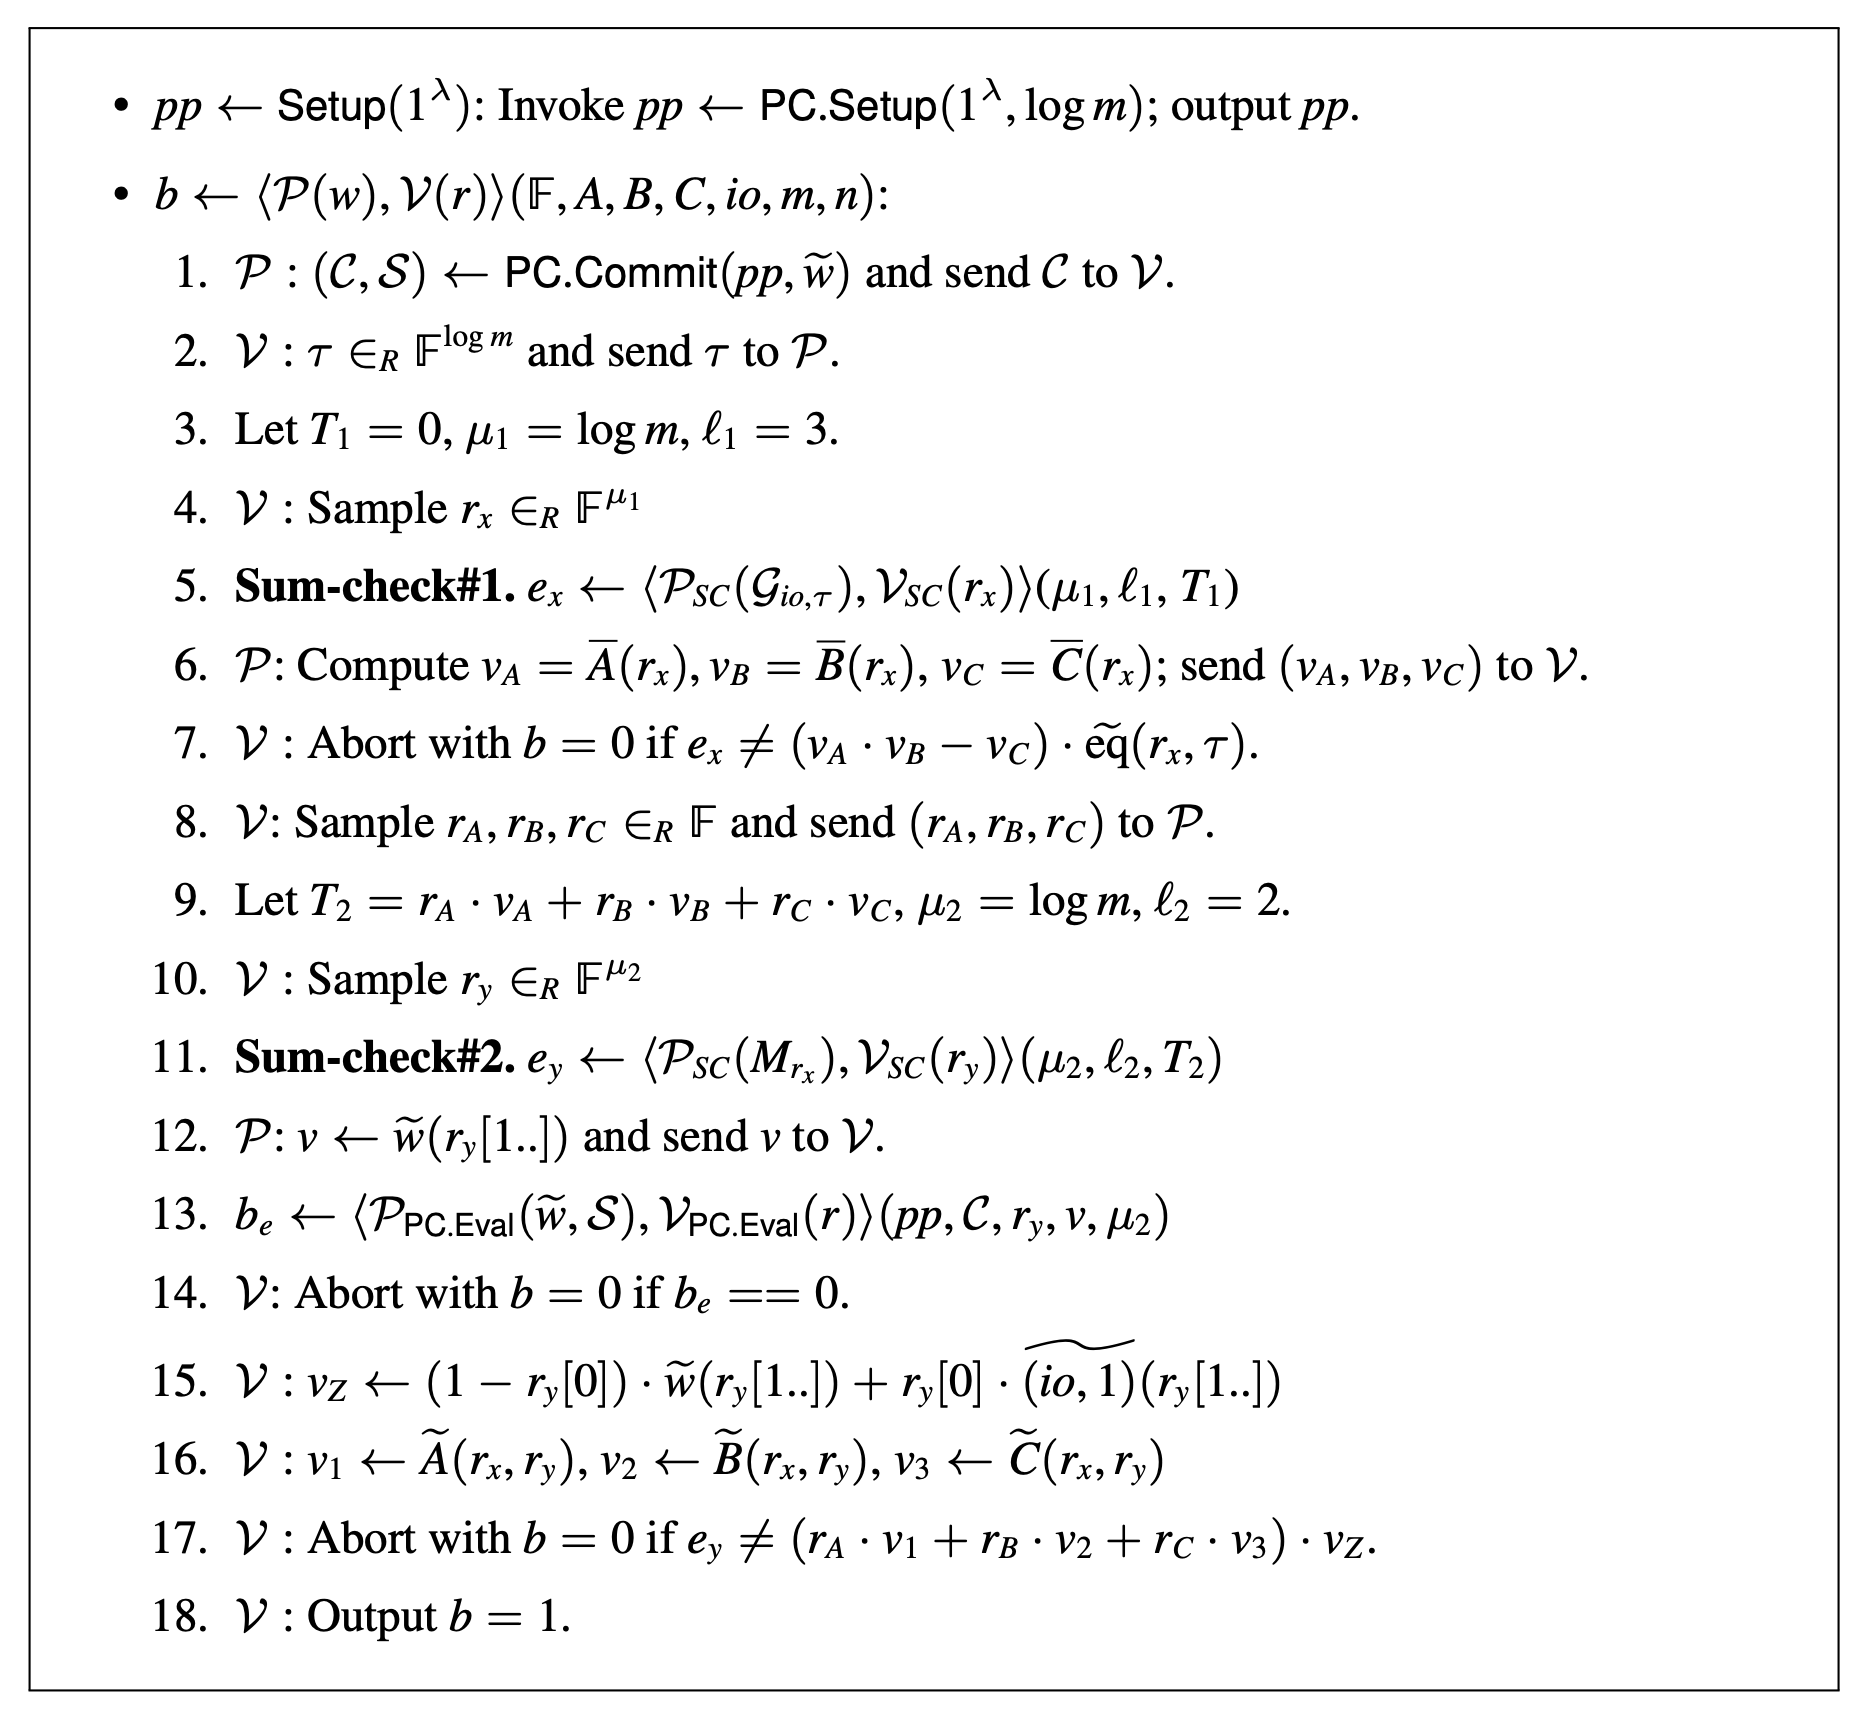
\includegraphics[width=\textwidth]{figures/spartan-description.png}
    \caption{The Spartan protocol description, from the original paper.}
    \label{fig:spartan_protocol}
\end{figure}

After stripping away the polynomial commitment scheme, the protocol has the following structure:

\begin{description}
    \item[Setup:] This step is part of the polynomial commitment scheme and is not part of the PIOP we formalize.
    \item[Interaction:] The interaction is between a prover $\IORProver$ with witness $w$ and a verifier $\IORVerifier$ with public inputs $(\mathbb{F}, A, B, C, \text{io}, m, n)$.
    \begin{enumerate}
        \item $\IORProver$: Sends oracle access to the multilinear extension of the witness, $\tilde{w}$, to $\IORVerifier$. In the original paper, this is a commitment $(C,S) \leftarrow \text{PC.Commit}(\text{pp}, \tilde{w})$.
        \item $\IORVerifier$: Samples a random challenge $\tau \in \mathbb{F}^{\log m}$ and sends it to $\IORProver$.
        \item Let $T_1 = 0$, $\mu_1 = \log m$, $\ell_1 = 3$. These are parameters for the first sum-check protocol.
        \item $\IORVerifier$: Samples a random challenge $r_x \in \mathbb{F}^{\mu_1}$.
        \item \textbf{Sum-check\#1.} A sum-check protocol is executed. The verifier receives the claimed evaluation $e_x$. The prover of the sum-check has oracle access to a polynomial $G_{io, \tau}$, and the verifier has oracle access to $r_x$. The parameters for this sub-protocol are $(\mu_1, \ell_1, T_1)$.
        \item $\IORProver$: Computes evaluations $v_A = \tilde{A}(r_x)$, $v_B = \tilde{B}(r_x)$, $v_C = \tilde{C}(r_x)$ and sends them to $\IORVerifier$. $\tilde{A}, \tilde{B}, \tilde{C}$ are multilinear extensions of the matrices $A, B, C$.
        \item $\IORVerifier$: Aborts if $e_x \neq (v_A \cdot v_B - v_C) \cdot \tilde{\text{eq}}(r_x, \tau)$. This is the verifier's check for the first sum-check.
        \item $\IORVerifier$: Samples random challenges $r_A, r_B, r_C \in \mathbb{F}$ and sends them to $\IORProver$.
        \item Let $T_2 = r_A \cdot v_A + r_B \cdot v_B + r_C \cdot v_C$, $\mu_2 = \log n$, $\ell_2 = 2$. These are parameters for the second sum-check protocol. Note: The image states $\mu_2 = \log m$, which is likely a typo and should be $\log n$.
        \item $\IORVerifier$: Samples a random challenge $r_y \in \mathbb{F}^{\mu_2}$.
        \item \textbf{Sum-check\#2.} Another sum-check protocol is executed. The verifier receives the claimed evaluation $e_y$.
        \item $\IORProver$: Computes $v \leftarrow \tilde{w}(r_y[1..])$ and sends $v$ to $\IORVerifier$.
        \item This step involves a polynomial commitment evaluation proof. In our PIOP formalization, this check is not needed as the verifier has direct oracle access to $\tilde{w}$.
        \item $\IORVerifier$: This step is part of the evaluation proof check, so it is omitted.
        \item $\IORVerifier$: Computes $v_Z \leftarrow (1 - r_y[0]) \cdot \tilde{w}(r_y[1..]) + r_y[0] \cdot \widetilde{(\text{io}, 1)}(r_y[1..])$. This reconstructs the evaluation of the combined input-witness vector polynomial $\tilde{z}$.
        \item $\IORVerifier$: Queries oracles for $\tilde{A}, \tilde{B}, \tilde{C}$ at $(r_x, r_y)$ to get $v_1, v_2, v_3$.
        \item $\IORVerifier$: Aborts if $e_y \neq (r_A \cdot v_1 + r_B \cdot v_2 + r_C \cdot v_3) \cdot v_Z$. This is the final check.
        \item $\IORVerifier$: Outputs 1.
    \end{enumerate}
\end{description}

\subsection{Formalization using IOR Composition}

We fix an R1CS size with $m$ constraints, $n_x$ public inputs and $n_w$ witness variables, and set
\[
  s = \lceil \log_2 m \rceil, \qquad t = \lceil \log_2 \max(n_x, n_w) \rceil + 1.
\]
The formalized PIOP pads the instance to $2^s$ constraints and to public-input and witness
vectors of length $2^{t-1}$, so that $z = (x, w)$ is indexed by $\{0,1\}^t$. It is the sequential
composition of seven oracle reductions; the bound in brackets is the round-by-round knowledge
error charged to each challenge of that stage, where $q = |\mathbb{F}|$.

\begin{definition}[Spartan PIOP]
    \label{def:spartan_reduction}
    \lean{Spartan.oracleReduction, Spartan.Assembly.stage,
      Spartan.PublicParams.forSize}
    \leanok
    \uses{def:oracle_reduction, def:sendsinglewitness_adapter, def:sumcheck_single_round}
    The Spartan oracle reduction is the composition of:
    \begin{enumerate}
        \item \textbf{Witness attachment} [$0$]: the prover sends the padded witness table as an
        oracle message, an instance of the adapter of Definition~\ref{def:sendsinglewitness_adapter}.
        \item \textbf{Zero-check} [$s/q$]: the verifier samples $\tau \in \mathbb{F}^{s}$, reducing
        the claim that every constraint holds (the multilinear extension of the residual
        $(Az) \circ (Bz) - Cz$ is zero) to the claim that this extension vanishes at $\tau$,
        equivalently
        $\sum_{x \in \{0,1\}^s} \tilde{\text{eq}}(\tau, x)\,((Az)_x (Bz)_x - (Cz)_x) = 0$.
        \item \textbf{First sum-check} [$3/q$]: sum-check of degree $3$ in $s$ rounds, ending at a
        point $r_x$.
        \item \textbf{Send evaluations} [$0$]: the prover sends $v_A, v_B, v_C$, and the verifier
        checks the first sum-check's final claim against them.
        \item \textbf{Batching} [$1/q$]: the verifier samples one challenge consisting of three
        independent coefficients $(r_A, r_B, r_C)$, forming the claim
        $T_2 = r_A v_A + r_B v_B + r_C v_C$.
        \item \textbf{Second sum-check} [$2/q$]: sum-check of degree $2$ in $t$ rounds, ending at
        a point $r_y$.
        \item \textbf{Terminal check} [$0$]: the verifier evaluates the second virtual polynomial at
        $r_y$ through the matrix and witness oracles and compares it with the final claim.
    \end{enumerate}
\end{definition}

\begin{theorem}[Perfect completeness]
    \label{thm:spartan_completeness}
    \lean{Spartan.perfectCompleteness}
    \leanok
    \uses{def:spartan_reduction, thm:sumcheck_perfect_completeness}
    The Spartan oracle reduction is perfectly complete from the original (unpadded) R1CS
    satisfiability relation to the trivial output relation.
\end{theorem}

\begin{theorem}[Round-by-round knowledge soundness]
    \label{thm:spartan_rbr}
    \lean{Spartan.rbrKnowledgeSoundnessWith, Spartan.challengeError}
    \leanok
    \uses{def:spartan_reduction, thm:sumcheck_rbr_knowledge_soundness_standard}
    The Spartan verifier is fixed-prefix round-by-round knowledge sound for the original R1CS
    relation, with each challenge charged the error of its stage listed in
    Definition~\ref{def:spartan_reduction}. The state function is the composition of the stage
    state functions, retaining every earlier rejecting check.
\end{theorem}

\begin{theorem}[Knowledge soundness]
    \label{thm:spartan_knowledge_soundness}
    \lean{Spartan.totalError, Spartan.error_ledger, Spartan.sum_challengeError,
      Spartan.knowledgeSoundnessWith, Spartan.straightlineExtractor,
      Spartan.foldExtractor_eq_straightlineExtractor,
      Spartan.knowledgeSoundnessWith_straightlineExtractor, Spartan.knowledgeSoundness,
      Spartan.knowledgeSoundness_clipped}
    \leanok
    \uses{thm:spartan_rbr, thm:rbr_knowledge_soundness_implies_knowledge_soundness}
    The per-challenge errors sum to
    \[
      \frac{s}{q} + s \cdot \frac{3}{q} + \frac{1}{q} + t \cdot \frac{2}{q} = \frac{4s + 2t + 1}{q}.
    \]
    The Spartan verifier is knowledge sound for the original R1CS relation with error
    $(4s + 2t + 1)/q$, and also with error $\min(1, (4s + 2t + 1)/q)$. The extractor obtained by
    folding the round-by-round extractors equals an executable straight-line extractor, which
    restricts the first message (the padded witness table) to the original witness coordinates.
\end{theorem}


% Copyright (c) 2026 ArkLib Contributors. All rights reserved.
% Released under Apache 2.0 license as described in the file LICENSE.

\section{FRI soundness}

We follow the March 27, 2026 revision of~\cite{GMW25}. The earlier
\href{https://github.com/zksecurity/simple-rbr-fri}{zkSecurity formalization}, by
Yoichi Hirai and Harmonic's Aristotle, with subsequent work by Pietro Monticone,
also informed the argument. ArkLib reuses its existing Reed--Solomon codes,
word-folding operations, mutual correlated agreement (MCA), and probability theory.

Let $D$ be a multiplicative coset of size $2^n$, let $m=2^k$ be a folding factor,
and let $D'=D^m$. Write $C=\mathrm{RS}(D,md)$ and
$C'=\mathrm{RS}(D',d)$, with $d>0$. For a word $f$ on $D$, write $f_j$ for the
coefficient words of its block interpolants, so that
$\operatorname{Fold}_\alpha(f)=\sum_{j<m}\alpha^j f_j$.

\begin{lemma}\label{lem:fri-coefficient-lift}
\lean{Fri.exists_codeword_agree_of_coefficients}
\leanok
If every $f_j$ agrees with a codeword in $C'$ on $T\subseteq D'$, then a single
codeword in $C$ agrees with $f$ on the whole preimage of $T$ under $x\mapsto x^m$.
\end{lemma}
\begin{proof}
\leanok
Choose degree-$<d$ polynomials $p_j$ witnessing agreement on $T$ and recombine them
as $p(X)=\sum_{j<m}X^j p_j(X^m)$. This polynomial has degree less than $md$.
Evaluation on every block above $T$ recovers its interpolant and hence the word.
\end{proof}

\begin{definition}\label{def:fri-folding-failure}
\lean{Fri.FoldingAgreementFailure}
\leanok
For a tradeoff parameter $\theta$, a challenge $\alpha$ is bad if there exists
$T\subseteq D'$ of size at least $(1-\theta)|D'|$ such that the folded word agrees
with $C'$ on $T$, but no codeword in $C$ agrees with $f$ on the whole preimage of $T$.
The parameter $\theta$ is independent of the input distance.
\end{definition}

\begin{theorem}\label{thm:fri-folding-error}
\lean{Fri.foldingAgreementFailure_prob_le_powers,
Fri.foldingAgreementFailure_prob_le_generalizedJohnson}
\leanok
\uses{def:fri-folding-failure,lem:fri-coefficient-lift}
For every fixed word $f$, the probability of a bad uniform challenge is at most
the MCA error of the powers generator $(1,\alpha,\ldots,\alpha^{m-1})$ for $C'$
at radius $\theta$.
\end{theorem}
\begin{proof}
\leanok
A bad challenge is an MCA failure for the coefficient words: if every coefficient
word agreed on the same $T$, \Cref{lem:fri-coefficient-lift} would lift the
agreement. No union bound over subsets is needed. The generalized-Johnson
specialization instantiates the existing powers-MCA bound from~\cite{BCGM25},
retaining all its field-size, slack, and radius assumptions.
\end{proof}

\begin{theorem}\label{thm:fri-query-error}
\lean{Fri.FoldTrace.query_soundness_distance}
\leanok
\uses{def:fri-folding-failure}
Fix a commitment trace with no bad folding challenge and let $\delta$ be the
initial word's relative distance from its Reed--Solomon code. The probability of
acceptance on $t$ independent uniform initial-domain queries is at most
$(1-\min\{\theta,\delta\})^t$.
\end{theorem}
\begin{proof}
\leanok
If the final word is not in its code, acceptance is impossible. Otherwise any
set of accepting initial positions of density at least $1-\theta$ agrees with
one original codeword: project the positions through each fold, observe that
density cannot decrease, and lift agreement backwards. Thus the accepting
density is at most $1-\min\{\theta,\delta\}$. Independent repetitions raise this
density to the $t$th power.
\end{proof}

\begin{theorem}\label{thm:fri-binding}
\lean{Fri.FoldTrace.exists_codeword_of_query_probability,
Fri.FoldTrace.exists_unique_codeword_agree_of_query_probability,
Fri.FoldTrace.interpolate_accepting_agrees,Fri.FoldTrace.not_accepts_of_disagreement}
\leanok
\uses{thm:fri-query-error}
For a safe trace with positive degree bound $d$ and $t>0$, suppose
$\delta\leq\theta$ and $\delta\leq 1-d/|D|$.
Acceptance probability at least $(1-\delta)^t$ implies that the initial word is
within relative distance $\delta$ of its code. A unique codeword agrees with it
on every accepting position. Interpolation on any $d$ accepting positions
recovers this codeword, and a query at a disagreement position forces rejection.
\end{theorem}
\begin{proof}
\leanok
The rate condition and $d>0$ give $\delta<1$, so positive acceptance implies a
valid final word. Positive $t$ gives accepting density at least $1-\delta$.
Since $\delta\leq\theta$, agreement lifts to an initial codeword within distance
$\delta$. Since $\delta\leq 1-d/|D|$, the accepting set has at least $d$ positions,
giving uniqueness. Lagrange interpolation supplies algebraic recovery on any
$d$ accepting positions. No extraction running-time bound is asserted.
\end{proof}

\begin{theorem}\label{thm:fri-soundness}
\lean{Fri.Spec.soundness,Fri.Spec.soundness_proximity,Fri.Spec.rbr_soundness}
\leanok
\uses{thm:fri-folding-error,thm:fri-query-error}
The specified FRI oracle reduction has round-by-round error equal to the
powers-MCA error at each folding challenge and $(1-\min\{\theta,\delta\})^t$
at its final query-vector challenge. Its ordinary soundness error is the sum of
these errors, against every adaptive prover. More strongly, this bounds any
acceptance when the input has distance at least $\delta$ from its initial code.
\end{theorem}
\begin{proof}
\leanok
Use the actual protocol transcript, including the retained committed words and
the terminal polynomial. A persistent state records that the input is valid or
a bad challenge has occurred. Prover messages cannot create this state.
The conditional probability of each fresh bad event is bounded by the appropriate
folding or query theorem. The executable verifier accepts exactly the final
query event, including the terminal degree guard, so it rejects whenever the
persistent state is false. This supplies round-by-round soundness through ArkLib's
fixed-prefix interface. Separately, induction over the actual stateful prover
execution accumulates the conditional errors and proves ordinary soundness.
\end{proof}

\paragraph{Executable specification and scope.}
The executable local consistency check is related to ArkLib's word fold by
\texttt{RoundConsistency.roundConsistencyCheck\_eq\_foldValue}, for arbitrary
oracle words. The specification retains all prior words, and checks the final
polynomial's degree before the query phase.
\texttt{Fri.Spec.reduction\_run} identifies the exact acceptance event of
\texttt{Fri.Spec.reduction}; the input-language bridge uses its original
computational-polynomial witness relation. The result concerns the interactive
oracle protocol, not Fiat--Shamir compilation or a concrete commitment scheme.

\subsection{Certified straightline extraction}

Write $N=2^n$, $b_i=2^{s_i}$, and $M=(\prod_i b_i)d$ for the initial
polynomial dimension, where all folding exponents and $d$ are positive and
$\sum_i s_i\leq n$.
The retained history contains arbitrary committed words, the folding challenges,
and a final computational polynomial. No intermediate honesty assumption is made.

\begin{definition}\label{def:fri-measured-extractor}
\lean{Fri.Spec.Extractor.extract,Fri.Spec.Extractor.extractProgram,
Fri.Spec.Extractor.extractHistory,Fri.Spec.Extractor.extractHistory_eq_profile}
\leanok
The named straightline extractor reads only the transcript prefix preceding the
query-vector challenge. It first rejects if the final polynomial has degree at
least $d$, before coefficient, domain, challenge, or word accesses. Otherwise it
scans every initial-domain position in order and applies the actual local checks.
It counts all accepting positions and caches the first $M$ nodes and initial-word
values. Fewer than $M$ acceptances yield failure. Otherwise it interpolates these
cached samples and returns the polynomial if its degree is less than $M$.
Its public result is the literal first projection of this measured program.
\end{definition}

\begin{theorem}\label{thm:fri-extractor-recovery}
\lean{Fri.Spec.Extractor.extractHistory_eq_some_of_safeHistory,
Fri.Spec.Extractor.extractHistory_eq_some_of_density}
\leanok
\uses{def:fri-measured-extractor,lem:fri-coefficient-lift}
Fix a safe retained history at threshold $\theta$, whose final polynomial has
degree less than $d$. Let $A$ be its accepting initial-domain positions. If
$N(1-\theta)\leq |A|$ and $M\leq |A|$, the named extractor returns a
polynomial of degree less than $M$ agreeing with the initial word on all of $A$.
Consequently, if $\tau\leq\theta$, $\tau\leq 1-M/N$, and
$N(1-\tau)\leq |A|$, the returned witness has relative distance at most $\tau$.
\end{theorem}
\begin{proof}
\leanok
Safe-history agreement lifting supplies one degree-bounded codeword agreeing on
$A$. The first $M$ cached nodes are distinct accepting positions, so polynomial
uniqueness identifies their measured interpolant with that codeword. The final
degree guard therefore succeeds. Disagreements are confined to the complement
of $A$, giving relative distance at most $1-|A|/N$.
\end{proof}

\begin{theorem}\label{thm:fri-knowledge-soundness}
\lean{Fri.Spec.knowledge_soundness_with,Fri.Spec.knowledge_soundness}
\leanok
\uses{thm:fri-folding-error,thm:fri-extractor-recovery}
Suppose $M\leq N$, $\delta\geq0$, and
$\min\{\theta,\delta\}\leq1-M/N$, including equality.
For every input statement, every adaptive prover, and every query count $l$, the
actual FRI reduction has straightline knowledge soundness with the named
extractor and error
\[
  \operatorname{soundnessError}
  =\sum_i\varepsilon_i(\theta)
    +\bigl(\max\{0,1-\min\{\theta,\delta\}\}\bigr)^l,
\]
where $\varepsilon_i(\theta)$ is the existing powers-MCA folding error.
The failure event includes both extraction failure and a returned witness outside
the original closed-ball input relation, when the accepted output witness is valid.
\end{theorem}
\begin{proof}
\leanok
Use fresh folding-failure events with the empty input language, so the adaptive
accumulation covers all inputs. For $0\leq\min\{\theta,\delta\}$,
conditional on a safe prefix, a failed extraction
and a valid final polynomial imply that the accepting density is less than
$1-\min\{\theta,\delta\}$, by \Cref{thm:fri-extractor-recovery}.
The query-vector probability is bounded by the corresponding $l$th power.
The logged-game bridge preserves private and shared oracle state and treats the
optional extraction result as a value, counting failure rather than aborting it.
If $\min\{\theta,\delta\}<0$, the query term is at least one and the bound is
vacuous. If $l=0$, this term is one as well. Neither case needs an additional
public assumption. Numerical estimates for the MCA terms retain their separate
field-size, slack, and radius hypotheses.
\end{proof}

\paragraph{Resource model.}
The arithmetic and immutable-input instruction handlers execute the very program
whose result defines the extractor. Field nodes are generated from at most two
domain reads by explicit measured powers; word-read addresses carry those nodes.
The profiles count repeated word, domain, challenge, coefficient, and cached-array
accesses; field addition, subtraction, multiplication, equality, and inversion;
and designated source-level control ticks. An inverse is one algebraic primitive.
Erased certificates carry the reference-domain and polynomial identities.
These counts exclude receipt or deserialization of retained functions, the cost
of evaluating those functions, allocation, machine index arithmetic, and field
bit complexity. Complete index enumeration prevents a claim of total $O(M)$
workspace here. The algebraic interpolation theorem above remains a separate
statement from these explicit measured programs.

\begin{theorem}\label{thm:fri-extractor-resources}
\lean{Fri.Spec.Extractor.profile_extractProgram_word_le,
Fri.Spec.Extractor.profile_extractProgram_apply_le,
Fri.Spec.Extractor.profile_extractProgram_inv_le,
Fri.Spec.Extractor.profile_extractProgram_domainRead_le,
Fri.Spec.Extractor.profile_extractProgram_challengeRead_le,
Fri.Spec.Extractor.profile_extractProgram_finalPolynomialRead,
Fri.Spec.Extractor.profile_extractProgram_add_sub_le,
Fri.Spec.Extractor.profile_extractProgram_mul_le,
Fri.Spec.Extractor.profile_extractProgram_eq_le}
\leanok
\uses{def:fri-measured-extractor}
Put $I(m)=100(m+1)^3$, $E(m)=(m+1)^2$, and
\[
  G=2(n+2)+\sum_i(4b_i+8)(n+1),\qquad
  J=1+\sum_i(n-s_i).
\]
For every retained history with $\sum_i s_i\leq n$, including rejected
histories, the measured extractor performs at most
\[
  N\left(\sum_i b_i+k\right)+M
  \quad\text{word reads},\qquad
  1+N\sum_i b_i(b_i-1)+M(M-1)
  \quad\text{inversions}.
\]
It performs at most two original-domain reads, at most $k+1$ folding-challenge
reads, and exactly one final-polynomial retrieval. Each of the combined
addition/subtraction count, the multiplication count, and the field-equality
count is bounded by
\[
  B=N\left[G+\sum_i\bigl(I(b_i)+E(b_i)+1\bigr)+E(d)\right]+I(M)+J.
\]
Every coefficient, node-cache, value-cache, and designated metadata coordinate
also obeys the explicit whole-program profile envelope.
\end{theorem}
\begin{proof}
\leanok
Add the initialization envelope, all $N$ scan-cell envelopes, and the final
interpolation envelope. The selected cache contributes at most $M$ extra word
reads. Every interpolation of size $m$ uses exactly $m(m-1)$ inverse requests.
Its combined additions/subtractions fit one $I(m)$ budget, as do its
multiplications and equality tests separately. Power-sum evaluation fits $E(m)$.
Only the final round evaluates the transmitted polynomial, giving one $E(d)$
per position. Explicit squaring and binary-power bounds fit $G$; initialization
multiplications fit $J$. All branches, including the initial degree rejection,
are included. No safe-history, honesty, radius, or $M\leq N$ premise is used.
\end{proof}

Under the actual reduction's $M\leq N$ constraint, these envelopes are
polynomial in $N$, rather than in $\log N$. The unit-access model above does
not bound bit complexity or cryptographic polynomial running time.

\section{Batched FRI}\label{sec:batched_fri}

Batched FRI tests $m+1$ words for proximity to one Reed--Solomon code by a single
FRI run on a random linear combination. Keep the notation of the previous section:
$\omega$ is a smooth coset FFT domain $D$ of size $2^n$ over a finite field of odd
characteristic, $s_0,\ldots,s_k\geq 1$ are the folding exponents, $d\geq 1$ is the
final degree bound, $l$ is the number of queries, and
$d_0:=2^{\sum_i s_i}\,d\leq 2^n$ is the initial degree bound. Write
$C_0=\mathrm{RS}(D,d_0)$. A generator $G:S\to\field^{m+1}$ supplies the batching
coefficients from a seed in a sampleable type $S$.

\begin{definition}[Batched FRI relation and reduction]\label{def:batched_fri}
\lean{BatchedFri.Spec.BatchingRound.inputRelation,
BatchedFri.Spec.BatchingRound.batchOracleReduction,
BatchedFri.Spec.batchedFRIreduction}
\leanok
\uses{def:proximity_generator,def:reed_solomon_code}
The input statement is $m+1$ oracle words $f_0,\ldots,f_m:D\to\field$; the witness
is $m+1$ polynomials $p_0,\ldots,p_m$ of degree less than $d_0$. For
$\delta\geq 0$, the input relation holds when some set $T\subseteq D$ with
$|T|\geq(1-\delta)2^n$ satisfies $f_i(x)=p_i(x)$ for every $i$ and every
$x\in T$. In the batching round the verifier sends one seed $c\in S$ and the
prover sends nothing. The output is the virtual oracle
$\sum_{i\leq m}G(c)_i f_i$, which feeds the initial FRI relation at the same
radius. Batched FRI is the append of this round with the FRI reduction of the
previous section.
\end{definition}

\begin{theorem}[Batched FRI soundness]\label{thm:batched_fri_soundness}
\lean{BatchedFri.Spec.batchedFRI_soundness,
BatchedFri.Spec.BatchingRound.soundness,
BatchedFri.Spec.BatchingRound.round_soundness}
\leanok
\uses{def:batched_fri,thm:fri-soundness}
Let $\delta,\varepsilon\geq 0$ and $\theta\in\mathbb{R}$, and assume
$\mathsf{caError}(G,C_0,\delta,\delta)\leq\varepsilon$. For every initial
distribution of the shared oracle state and every implementation of that oracle,
the Batched FRI verifier is sound from the language of the input relation at
radius $\delta$ to the language of the FRI output relation at radius $\delta$,
with error
\[
  \varepsilon+\sum_i\varepsilon^{\mathrm{fold}}_i+(1-\min\{\theta,\delta\})_+^{\,l},
\]
where the last two terms are the FRI soundness error of
Theorem~\ref{thm:fri-soundness}. The batching round alone is round-by-round sound
with error $\varepsilon$.
\end{theorem}

\begin{theorem}[Batched FRI completeness]\label{thm:batched_fri_completeness}
\lean{BatchedFri.Spec.batchedFRI_perfectCompleteness}
\leanok
\uses{def:batched_fri}
For every generator, query count and shared-oracle implementation, Batched FRI is
perfectly complete from the input relation at radius $0$ to the FRI output
relation at radius $0$.
\end{theorem}

The generator hypothesis is discharged for four generators. Write
$\rate$ for the rate of $C_0$, and $\varepsilon_{\mathrm{BCIKS}}(\delta)$ for the
error that equals $2^n/|\field|$ when $\delta\leq(1-\rate)/2$, equals
$d_0^2/\bigl((2\min\{1-\sqrt\rate-\delta,\sqrt\rate/20\})^7|\field|\bigr)$ when
$(1-\rate)/2<\delta<1-\sqrt\rate$, and is $0$ otherwise.

\begin{theorem}[Batched FRI with concrete generators]\label{thm:batched_fri_generators}
\lean{BatchedFri.Spec.batchedFRI_soundness_affineSpace,
BatchedFri.Spec.batchedFRI_soundness_powers,
BatchedFri.Spec.batchedFRI_soundness_multilinear,
BatchedFri.Spec.batchedFRI_soundness_multilinear_johnson}
\leanok
\uses{thm:batched_fri_soundness}
Under the hypotheses of Theorem~\ref{thm:batched_fri_soundness} without the
$\mathsf{caError}$ assumption, the soundness error is the FRI error plus the
following batching error.
\begin{itemize}
  \item Affine space $c\mapsto(1,c_1,\ldots,c_m)$, $c\in\field^m$, with
    $0<\delta<1-\sqrt\rate$: $\varepsilon_{\mathrm{BCIKS}}(\delta)$.
  \item Powers $c\mapsto(1,c,\ldots,c^m)$, $c\in\field$, with
    $0<\delta<1-\sqrt\rate$: $m\cdot\varepsilon_{\mathrm{BCIKS}}(\delta)$.
  \item Multilinear monomials in $t$ variables, so $m+1=2^t$, with $\delta>0$
    at most the relative unique decoding radius of $C_0$:
    $t\cdot 2^n/|\field|$.
  \item The same multilinear generator, with $\delta_{\min}$ the relative minimum
    distance of $C_0$, $0<\eta<\delta_{\min}$ and
    $0<\delta\leq 1-(1-\delta_{\min}+\eta)^{1/3}$: $t$ times the affine-line
    MCA error
    \[
      \frac{1}{|\field|}\left(\frac{2^n+6}{\eta}
      +\frac{2}{\eta\bigl((1-\delta_{\min}+\eta)^{1/3}
      -(1-\delta_{\min}+\eta)^{1/2}\bigr)}\right),
    \]
    truncated below at $0$.
\end{itemize}
\end{theorem}

Knowledge soundness of Batched FRI is not formalized: the batching round has no
extractor.


% Copyright (c) 2025 ArkLib Contributors. All rights reserved.
% Released under Apache 2.0 license as described in the file LICENSE.
% Authors: Poulami Das (Least Authority)

\section{STIR}

\subsection{Tools for Reed Solomon codes}
\subsubsection{Random linear combination as a proximity generator}\label{sec:proximity_gap}

\begin{theorem}\label{thm:proximity_gap}
\lean{STIR.proximity_gap}
\leanok
\uses{def:distance_from_code,def:reed_solomon_code,def:list_close_codewords}
    Let $\code := \rscode[\field,\evaldomain,\degree]$ be a Reed Solomon code with $\degree\ge1$ and rate $\rate:=\frac{\degree}{|\evaldomain|}$ and let $B^*(\rate):=\sqrt{\rate}$. For every $\distance \in (0,1 - B^*(\rate))$ and functions $f_0,\ldots,f_{m-1} : \evaldomain \to \field$, if
    \[
    \Pr_{r\leftarrow\field}\!\Bigl[
      \Delta\Bigl(\sum_{j=0}^{m-1} r^j\cdot {f_j},\rscode[\field,\evaldomain,\degree]\Bigr)
      \le \delta
    \Bigr]>\err^*(\degree,\rate,\distance,m),
    \]
    then there exists a subset $S \subseteq \evaldomain$ with $|S| \ge (1 - \delta)\cdot|\evaldomain|$,
    and for every $i \in \{0,\ldots,m-1\}$, there exists $u \in \rscode[\field,\evaldomain,\degree]$ such that $f_i(S) = u(S)$.

    \medskip

    \noindent
    Above, $\err^*(\degree,\rate,\distance,m)$ is defined as follows:
    \begin{itemize}
        \item if $\distance \in \left(0,\frac{1-\rate}{2}\right]$ then
            \[
                \err^*(\degree,\rate,\distance,m)=\frac{(m-1)\cdot \degree}{\rate\cdot|\field|}
            \]
        \item if $\distance \in \Bigl(\frac{1-\rate}{2}, 1-\sqrt{\rate}\Bigr)$ then
        \[
            \err^*(\degree,\rate,\distance,m)=\frac{(m-1)\cdot {\degree}^2}{|\field|\cdot{\Bigl(2\cdot\min\{1-\sqrt{\rate}-\distance,\frac{\sqrt{\rate}}{20}\}\Bigr)}^7}
        \]
    \end{itemize}
\end{theorem}

\begin{proof}
\leanok
For an empty family, take the whole evaluation domain. Otherwise write $m=k+1$ and apply
correlated agreement for affine curves from \cite{BCIKS20}. In the admissible distance range,
the error above equals $k$ times the correlated-agreement error bound, in both the unique-decoding
and Johnson regimes. The resulting joint agreement gives the common set $S$.
\end{proof}

\subsubsection{Univariate Function Quotienting}\label{sec:quotienting}

In the following, we start by defining the \emph{quotient} of a univariate function.
\begin{definition}\label{def:quotient}
\lean{Quotienting.funcQuotient}
\leanok
    Let $f:\evaldomain\to\field$ be a function, $S\subseteq\field$ be a finite set, and $\mathsf{Ans},\mathsf{Fill}: S\rightarrow\field$ be functions. Let $\hat{\mathsf{Ans}}\in\field^{<|S|}[X]$ be the unique polynomial of degree less than $|S|$ with $\hat{\mathsf{Ans}}(x)=\mathsf{Ans}(x)$ for every $x\in S$ (the zero polynomial when $S$ is empty), and let $\hat{V}_S(X):=\prod_{s\in S}(X-s)$, the unique monic polynomial of degree $|S|$ vanishing on $S$.
    The \emph{quotient function} $\mathsf{Quotient}\bigl(f,S,\mathsf{Ans},\mathsf{Fill}\bigr): \evaldomain\to\field$
    is defined as follows:

    \[
    \forall x \in \evaldomain, \quad
    \mathsf{Quotient}\bigl(f, S, \mathsf{Ans}, \mathsf{Fill} \bigr)(x)
    :=
    \left\{
    \begin{array}{ll}
        \mathsf{Fill}(x)
        & \text{if } x \in S \\[6pt]
        \dfrac{f(x) - \hat{\mathsf{Ans}}(x)}{\hat{V}_S(x)}
        & \text{otherwise}
    \end{array}
    \right.
    \]

\end{definition}

Next we define the polynomial quotient operator, which quotients a polynomial relative to its output on evaluation points. The polynomial quotient is a polynomial of lower degree.

\begin{definition}\label{def:poly_quotient}
\lean{Quotienting.polyQuotient}
\leanok
    Let $\hat{f}\in\field^{<\degree}[X]$ be a polynomial and $S\subseteq\field$ be a finite set with $|S|\le\degree$, and let $\hat{V}_S(X):=\prod_{s\in S}(X-s)$, the unique monic polynomial of degree $|S|$ vanishing on $S$. The \emph{polynomial quotient} $\mathsf{PolyQuotient}(\hat{f},S)\in\field^{<d-|S|}[X]$ is defined as follows:
    \[
            \mathsf{PolyQuotient}(\hat{f},S)(X):=\frac{\hat{f}(X)-\hat{\mathsf{Ans}}(X)}{\hat{V}_S(X)}
    \]
where $\hat{\mathsf{Ans}}\in\field^{<|S|}[X]$ is the unique polynomial of degree less than $|S|$ interpolating $\hat{f}$ on $S$.
\end{definition}

The following lemma, implicit in prior works, shows that if the function is ``quotiented by the wrong value'', then its quotient is far from low-degree.

\begin{lemma}\label{lemma:quotienting}
\lean{Quotienting.quotienting}
\leanok
\uses{def:quotient,def:reed_solomon_code,def:distance_from_code,def:list_close_codewords}
    Let $f:\evaldomain\rightarrow\field$ be a function, $\degree\in\N$ be the degree parameter with $\degree\le|\evaldomain|$, $\distance\in(0,1)$
    be a distance parameter, $S\subseteq\field$ be a set with $|S|<\degree$, and $\mathsf{Ans},\mathsf{Fill}:S\rightarrow\field$ are functions. Suppose that for every $u\in\listcode(f,\degree,\distance)$ there exists $x\in S$ with $\hat{u}(x)\neq\mathsf{Ans}(x)$. Then

    \[
            \Delta(\mathsf{Quotient}(f,S,\mathsf{Ans},\mathsf{Fill}),\rscode[\field,\evaldomain,\degree-|S|])+\frac{|T|}{|\evaldomain|}>\distance,
    \]
    where $T:=\{x\in\evaldomain\cap S: \hat{\mathsf{Ans}}(x)\neq f(x)\}$.
\end{lemma}

\subsubsection{Out of domain sampling}\label{sec:out_of_domain_smpl}
\begin{lemma}\label{lemma:out_of_domain_smpl}
\lean{OutOfDomSmpl.out_of_dom_smpl_1, OutOfDomSmpl.out_of_dom_smpl_2}
\leanok
\uses{def:reed_solomon_code,def:list_decodable,def:list_close_codewords}
    Let $\field$ be a finite field and $\evaldomain\subseteq\field$ an evaluation domain with $|\evaldomain|<|\field|$, so that $\field\setminus\evaldomain$ is nonempty. Let $f:\evaldomain\rightarrow\field$ be a function, $\degree\in\N$ be a degree parameter, $s\in\N$ be a repetition parameter, $\distance\ge0$ be a distance parameter and $l\ge0$ a real list-size bound. If $\rscode[\field,\evaldomain,\degree]$ is $(\distance,l)$-list decodable, then
        \[
        \begin{array}{rcl}
        \Pr_{\substack{r_0, \ldots, r_{s-1} \gets \field \setminus \evaldomain}}
        \left[
        \begin{array}{c}
            \exists \text{ distinct } u, u' \in \listcode(f, \degree, \distance): \\
            \forall i \in [s],\ \hat{u}(r_i) = \hat{u}'(r_i)
        \end{array}
        \right]
        & \leq & \frac{l\,(l-1)}{2} \cdot \left( \frac{\degree - 1}{|\field| - |\evaldomain|} \right)^s \\
        & \leq & \left( \frac{l^2}{2} \right) \cdot \left( \frac{\degree}{|\field| - |\evaldomain|} \right)^s
        \end{array}
        \]
    Here $l-1$ is truncated at $0$, and the $r_i$ are independent and uniform on
    $\field\setminus\evaldomain$.
\end{lemma}

\subsubsection{Folding univariate functions}\label{sec:folding_uf}
STIR relies on $k$-wise folding of functions and polynomials - this is similar to prior works, although presented in a slightly different form. As shown below, folding a function preserves proximity from the Reed-Solomon code with high probability. The folding operator is based on the following fact, decomposing univariate polynomials into bivariate ones.

\begin{lemma}\label{fact:poly_folding}
\lean{Polynomial.FoldingPolynomial.foldingPolynomial,
Polynomial.FoldingPolynomial.substitution_property_of_folding_polynomial,
Polynomial.FoldingPolynomial.folding_polynomial_deg_x,
Polynomial.FoldingPolynomial.folding_polynomial_deg_y_bound,
Polynomial.FoldingPolynomial.folding_polynomial_is_unique,
Polynomial.FoldingPolynomial.folding_polynomial_deg_x_bound,
Polynomial.FoldingPolynomial.folded_poly_degree_bound}
\leanok
Given a non-constant polynomial $\hat{q}\in\field[X]$:
\begin{itemize}
        \item For every univariate polynomial $\hat{f}\in\field[X]$, there exists a unique bivariate polynomial $\hat{Q}\in\field[X,Y]$ with:
        \[
          \polydeg_X(\hat{Q}) := \left\lfloor \frac{\polydeg(\hat{f})}{\polydeg(\hat{q})} \right\rfloor,\quad \polydeg_Y(\hat{Q}) < \polydeg(\hat{q})
        \]
        such that $\hat{f}(Z)=\hat{Q}(\hat{q}(Z),Z)$. Observe that if $\polydeg(\hat{f})<t\cdot\polydeg(\hat{q})$ then
        $\polydeg_X(\hat{Q})<t$.

        \item For every $\hat{Q}[X,Y]$ with $\polydeg_X(\hat{Q})<t$ and $\polydeg_Y(\hat{Q})<\polydeg(\hat{q})$, the polynomial $\hat{f}(Z)=\hat{Q}(\hat{q}(Z),Z)$ has degree $\polydeg(\hat{f})<t\cdot\polydeg(\hat{q})$.
\end{itemize}
\end{lemma}

Moreover, $\hat{Q}$ can be computed efficiently given $\hat{f}$ and $\hat{q}$; the formalization
defines it by repeated division by $\hat{q}$.

Below, we define folding of a polynomial followed by folding of a function.
\begin{definition}\label{def:poly_folding}
\lean{Polynomial.FoldingPolynomial.polyFold,
Polynomial.FoldingPolynomial.polyFold_natDegree_le}
\leanok
\uses{fact:poly_folding}
    Given a polynomial $\hat{f}\in\field[X]$, a folding parameter $k\in\N$ with $k\ge1$ and $r\in\field$, we define a polynomial $\mathsf{PolyFold}(\hat{f},k,r)\in\field[X]$ as follows. Let $\hat{Q}[X,Y]$ be the bivariate polynomial derived from $\hat{f}$ using \Cref{fact:poly_folding} with the non-constant polynomial $\hat{q}(X):=X^k$. Then $\mathsf{PolyFold}(\hat{f},k,r)(X):=\hat{Q}(X,r)$. Its degree is at most $\lfloor\polydeg(\hat{f})/k\rfloor$.
\end{definition}

\begin{definition}\label{def:fn_folding}
\lean{ProximityGap.foldWord}
\leanok
Let $f:\evaldomain\rightarrow\field$ be a function, $k\in\N$ a folding parameter and $\alpha\in\field$. For every $x\in{\evaldomain}^k$, let $\hat{p}_x\in\field^{<k}[X]$ be the polynomial where $\hat{p}_x(y)=f(y)$ for every $y\in{\evaldomain}$ such that $y^k=x$. We define $\mathsf{Fold}(f,k,\alpha):{\evaldomain}^k\rightarrow\field$ as follows.
\[
    \mathsf{Fold}(f,k,\alpha)(x):=\hat{p}_x(\alpha).
\]
In order to compute $\mathsf{Fold}(f,k,\alpha)(x)$ it suffices to interpolate the $k$ values $\{f(y):y\in\evaldomain\text{ s.t. }y^k=x\}$ into the polynomial $\hat{p}_x$ and evaluate this polynomial at $\alpha$.
The formalization takes $\evaldomain$ to be a smooth coset FFT domain of size $2^n$ and a folding
parameter of the form $2^k$.
\end{definition}

The following lemma shows that the distance of a function is preserved under folding. If a functions $f$ has distance $\distance$ to a Reed-Solomon code then, with high probability over the choice of folding randomness, its folding also has a distance of $\distance$ to the ``$k$-wise folded'' Reed-Solomon code.

\begin{lemma}\label{lemma:folding}
\lean{ProximityGap.folding_preserves_distance}
\leanok
\uses{def:reed_solomon_code,def:fn_folding,def:distance_from_code}
    Let $\evaldomain$ be a smooth coset FFT domain of size $2^n$, let $\degree=2^{d}$ and let the
    folding parameter be $2^{k}$ with $1\le k\le d\le n$. Let $\rate:=\frac{\degree}{|\evaldomain|}$.
    For every function $f:\evaldomain\rightarrow\field$ and distance parameter
    $\distance\in(0,\min\{\Delta(f,\rscode[\field,\evaldomain,\degree]),1-{\mathsf{B}}^*(\rate)\})$,
    \[
        \Pr_{r^{\mathsf{fold}}\gets\field}[\Delta(\mathsf{Fold}(f,2^k,r^{\mathsf{fold}}),\rscode[\field,{\evaldomain}^{2^k}, \degree/2^k])\le\distance]\le\err^*(\degree/2^k,\rate,\distance,2^k).
    \]
    Above, ${\mathsf{B}}^*$ and ${\err}^*$ are the proximity bound and error (respectively) described in \Cref{sec:proximity_gap}.
\end{lemma}

\subsubsection{Combine functions of varying degrees}\label{sec:combine}
We show a new method for combining functions of varying degrees with minimal proximity require- ments using geometric sums. We begin by recalling a fact about geometric sums.

\begin{lemma}\label{fact:geometric_sum}
\lean{Combine.geometric_sum_units}
\leanok
    Let $\field$ be a field, $r\in\field^\times$ be a nonzero field element, $a\in\N$ be a natural number. Then
    \[
    \sum_{i=0}^{a} r^i :=
    \left\{
    \begin{array}{ll}
        \displaystyle\left(\frac{1 - r^{a+1}}{1 - r}\right)
        & \text{if } r \neq 1 \\[6pt]
        a + 1
        & \text{if } r = 1
    \end{array}
    \right.
    \]

\end{lemma}

\begin{definition}\label{def:combine}
\lean{Combine.combine}
\leanok
    Given target degree $\degree^*\in\N$, shifting parameter $r\in\field$, functions $f_0,\ldots,f_{m-1}:\evaldomain\rightarrow\field$, and degrees $0\leq \degree_0,\ldots,\degree_{m-1}\leq {\degree}^*$, we define $\combine(\degree^*,r,(f_0,\degree_0),\ldots,(f_{m-1},\degree_{m-1})):\evaldomain\rightarrow\field$ as follows:
        \[
        \begin{array}{rcl}
        \combine(\degree^*, r, (f_0, \degree_0), \ldots, (f_{m-1}, \degree_{m-1}))(x)
        & := & \displaystyle\sum_{i=0}^{m-1} r_i \cdot f_i(x) \cdot \left( \sum_{l=0}^{\degree^* - \degree_i} (r \cdot x)^l \right) \\[10pt]
        & = & \left\{
        \begin{array}{ll}
            \displaystyle\sum_{i=0}^{m-1} r_i \cdot f_i(x) \cdot \left( \dfrac{1 - (x r)^{\degree^* - \degree_i + 1}}{1 - x r} \right)
            & \text{if } x \cdot r \neq 1 \\[8pt]
            \displaystyle\sum_{i=0}^{m-1} r_i \cdot f_i(x) \cdot (\degree^* - \degree_i + 1)
            & \text{if } x \cdot r = 1
        \end{array}
        \right.
        \end{array}
        \]

Above, $r_i:=r^{i+\sum_{j<i}(\degree^*-\degree_j)}$.
\end{definition}

\begin{definition}\label{def:deg_corr}
\lean{Combine.degCor}
\leanok
\uses{def:combine,def:reed_solomon_code,def:distance_from_code}
    Given target degree $\degree^*\in\N$, shifting parameter $r\in\field$, function $f:\evaldomain\rightarrow\field$, and degree $0\leq\degree\leq\degree^*$, we define $\degcorr(\degree^*,r,f,\degree)$ as follows.
    \[
    \begin{array}{rcl}
    \degcorr(\degree^*, r, f, \degree)(x)
    & := & \displaystyle f(x) \cdot \left( \sum_{l=0}^{\degree^* - \degree} (r \cdot x)^l \right) \\[10pt]
    & = & \left\{
    \begin{array}{ll}
        \displaystyle f(x) \cdot \left( \dfrac{1 - (x r)^{\degree^* - \degree + 1}}{1 - x r} \right)
        & \text{if } x \cdot r \neq 1 \\[8pt]
        \displaystyle f(x) \cdot (\degree^* - \degree + 1)
        & \text{if } x \cdot r = 1
    \end{array}
    \right.
    \end{array}
    \]


(Observe that $\degcorr(\degree^*,r,f,\degree)=\combine(\degree^*,r,(f,\degree))$.)
\end{definition}

Below it is shown that combining multiple polynomials of varying degrees can be done as long as the proximity error is bounded by $(\min{\{1-{\mathsf{B}}^*(\rate),1-\rate-1/|\evaldomain|\}})$.

\begin{lemma}\label{lemma:combine}
\lean{Combine.combine_theorem}
\leanok
\uses{def:reed_solomon_code,def:combine,def:deg_corr,thm:proximity_gap}
    Let $\degree^*\ge1$ be a target degree, $f_0,\ldots,f_{m-1}:\evaldomain\rightarrow\field$ be functions, $0\leq \degree_0,\ldots,\degree_{m-1}\leq \degree^*$ be degrees, $\distance\in(0,\min{\{1-{\mathsf{B}}^*(\rate),1-\rate-1/|\evaldomain|\}})$ be a distance parameter, where $\rate=\degree^*/|\evaldomain|$. If
    \[
        \Pr_{r\gets\field}[\Delta(\combine(\degree^*,r,(f_0,\degree_0),\ldots,(f_{m-1},\degree_{m-1})),\rscode[\field,\evaldomain,\degree^*])\le\distance]>\err^*(\degree^*,\rate,\distance,m\cdot(\degree^*+1)-\sum_{i=0}^{m-1}\degree_i),
    \]
    then there exists $S\subseteq \evaldomain$ with $|S|\geq(1-\distance)\cdot|\evaldomain|$, and
    \[
        \forall i\in\{0,\ldots,m-1\},\exists u\in\rscode[\field,\evaldomain,\degree_i], f_i(S)=u(S).
    \]
    Note that this implies $\Delta(f_i,\rscode[\field,\evaldomain,\degree_i])\le\distance$ for every $i$. Above, ${\mathsf{B}}^*$ and ${\err}^*$ are the proximity bound and error (respectively) described in the proximity gap theorem.
\end{lemma}

\subsection{STIR Section 5 targets}

Construction 5.2, Lemma 5.4 and Theorem 5.1 of \cite{ACFY24stir} remain unformalized.
The statements below record the paper's intended bounds. ArkLib formalizes the construction's
parameter and domain conditions in \texttt{StirIOP.ParamConditions}, together with the codeword
completeness relation and strict soundness relation, but has no concrete STIR prover and verifier.
A protocol must be fixed by Construction 5.2 before its distances and list sizes are chosen.

\begin{theorem}[STIR Main Theorem, unformalized target]\label{thm:stir}
\uses{def:reed_solomon_code,lemma:rnd_by_rnd_soundness}
    Consider the following ingredients:
    \begin{itemize}
        \item A security parameter $\lambda\in\N$.
        \item A Reed-Solomon code $\rscode[\field,\evaldomain,\degree]$ with $\rate:=\frac{\degree}{|\evaldomain|}$ where $\degree$ is a power of $2$, and $\evaldomain$ is a smooth domain.
        \item A proximity parameter $\distance\in(0,1-1.05\cdot\sqrt{\rate})$.
        \item A folding parameter $k\in\N$ that is power of $2$ with $k\geq 4$.
    \end{itemize}
If $|\field|=\Omega(\frac{\lambda\cdot2^\lambda\cdot\degree^2\cdot{|\evaldomain|}^{3.5}}{\log(1/\rate)})$, there is a public-coin IOPP for $\rscode[\field,\evaldomain,\degree]$ with the following parameters:
\begin{itemize}
    \item Round-by-round soundness error $2^{-\lambda}$.
    \item Round complexity: $M:=O(\log_k{\degree})$.
    \item Proof length: $|\evaldomain|+O_k(\log{\degree})$.
    \item Query complexity to the input: $\frac{\lambda}{-\log{(1-\distance)}}$.
    \item Query complexity to the proof strings: $O_k(\log{\degree}+\lambda\cdot\log{\Big(\frac{\log{\degree}}{\log{1/\rate}}\Big)})$.
\end{itemize}
\end{theorem}

\begin{remark}[Formalization target]
The exponent $3.5$ of the field size is the one of the January 2025 revision of ePrint 2024/390
\cite{ACFY24stir} (Theorem 5.1 and Appendix C.1). The constants in the $\Omega$ and $O$ bounds must
be uniform in the protocol parameters; $O_k$ constants may depend on $k$.
A formalization must establish the concrete protocol's round, proof-length and both query bounds,
counting $k$ grouped points as one symbol as in the paper. Numerical error and proof-length bounds
for an arbitrary protocol permit an exhaustive exact-membership verifier and do not characterize
this theorem. Appendix C.1 also includes a field-size dependence on
$1/(-\log(1-\distance'))$, absent from the displayed Theorem 5.1; the parameter analysis must
resolve this discrepancy.
\end{remark}

\begin{lemma}[Round-by-round soundness, unformalized target]\label{lemma:rnd_by_rnd_soundness}
\uses{def:reed_solomon_code,def:list_decodable,lemma:folding,lemma:out_of_domain_smpl,lemma:quotienting,lemma:combine}
    Consider $(\field,M,\degree,k_0,\ldots,k_M,\evaldomain_0,\ldots,\evaldomain_M,t_0,\ldots,t_M,s)$ and for every $i\in\{0,\ldots,M\}$, let $\degree_i:=\frac{\degree}{\prod_{j<i}k_j}$ and $\rate_i:=\degree_i/|\evaldomain_i|$, where, as in Construction~5.2 of \cite{ACFY24stir}, $\degree$ and $k_0,\ldots,k_M$ are powers of $2$ with $\degree\ge\prod_i k_i$, each $\evaldomain_i$ is a smooth domain with $|\evaldomain_i|>\degree_i$, and $t_i+1\le\degree_{i+1}$ for every $i<M$. For every $f\notin\rscode[\field,\evaldomain_0,\degree_0]$ and every $\distance_0,\ldots,\distance_M$ where
    \begin{itemize}
        \item $\distance_0\in(0,\Delta(f,\rscode[\field,\evaldomain_0,\degree_0])]\cap(0,1-{\mathsf{B}}^*(\rate_0))$
        \item for every $0<i\leq M$: $\distance_i\in(0,\min{\{1-\rate_i-\frac{1}{|\evaldomain_i|},1-{\mathsf{B}^*(\rate_i)}\}})$, and
        \item for every $0<i\leq M$: $\rscode[\field,\evaldomain_i,\degree_i]$ is $(\distance_i,l_i)$-list decodable,
    \end{itemize}
    The STIR IOPP of Construction~5.2 with these fixed parameters has round-by-round soundness error $(\epsilon^{\mathsf{fold}},\epsilon^{\mathsf{out}}_1,\epsilon^{\mathsf{shift}}_1,\ldots,\epsilon^{\mathsf{out}}_M,\epsilon^{\mathsf{shift}}_M,\epsilon^{\mathsf{fin}})$ where:
    \begin{itemize}
        \item $\epsilon^{\mathsf{fold}}\leq\err^*(\degree_0/k_0,\rate_0,\distance_0,k_0)$.
        \item $\epsilon^{\mathsf{out}}_i\leq\frac{l^2_i}{2}\cdot{\big(\frac{\degree_i}{|\field|-|\evaldomain_i|}\big)}^s$
        \item $\epsilon^{\mathsf{shift}}_i\leq {(1-\distance_{i-1})}^{t_{i-1}}+\err^*(\degree_i,\rate_i,\distance_i,t_{i-1}+s)+\err^*(\degree_i/k_i,\rate_i,\distance_i,k_i)$.
        \item $\epsilon^{\mathsf{fin}}\leq{(1-\distance_M)}^{t_M}$.
    \end{itemize}
    Above, ${\mathsf{B}}^*$ and ${\err}^*$ are the proximity bound and error (respectively) described in \Cref{sec:proximity_gap}.
\end{lemma}

\begin{remark}[Formalization target]
The protocol must be determined by Construction~5.2 before the distances $\distance_i$ and list
sizes $l_i$ are chosen. Its completeness relation consists of codewords, while its soundness
language is the strict distance relation: the bad inputs include distance exactly $\distance_0$.
Each component of the displayed error vector must bound its corresponding challenge, including
final verification when $M=0$. Construction~5.2 uses $2M+1$ interactive rounds and a randomized
final decision; a faithful representation must retain the prescribed uniform sampling from
$\field\setminus\evaldomain_i$ and folded evaluation domains. The current fixed-length field-vector
challenge representation does not in general realize these distributions.
\end{remark}


% Copyright (c) 2025 ArkLib Contributors. All rights reserved.
% Released under Apache 2.0 license as described in the file LICENSE.
% Authors: Poulami Das (Least Authority)

\section{WHIR}

\subsection{Tools for Reed Solomon codes}

\subsubsection{Mutual Correlated Agreement as a Proximity Generator}

\begin{definition}\label{def:proximity_generator}
\lean{ProximityGap.caError}
\leanok
\uses{def:linear_code,def:distance_from_code}
Let $\code\subseteq \field^{\evaldomain}$ be a linear code. We say that $\mathsf{Gen}$ is a proximity generator for $\code$ with proximity bounds ${\bound}$ and $\err$ if the following implication holds for $f_0,\ldots,f_{\parl-1} : \evaldomain \rightarrow \field$ and $\delta\in(0,1-{\bound}(\rate,\parl))$. If
\begin{align*}
    \Pr_{r_0,\ldots,r_{\parl-1}\leftarrow \gen}[\Delta(\sum_{i\in[0,(\parl-1)]} r_i \cdot f_i, \code) \le \delta] > err(\code,\parl,\delta),
\end{align*}
then there exists $S\subseteq \evaldomain$, $|S|\ge(1-\delta)\cdot|\evaldomain|$, and
$\forall i \in [0, (\parl-1)]$, $\exists u \in \code, \forall x \in S$, $f_i(x)=u(x)$.

The formalization records the least admissible error as a function: the correlated-agreement
error $\mathsf{caError}(\gen,\code,\delta,\delta)$ is the supremum, over word stacks
$(f_0,\ldots,f_{\parl-1})$ that are not jointly $\delta$-close to $\code$, of the probability
above. Thus $\gen$ is a proximity generator with error $\err$ at $\delta$ exactly when
$\mathsf{caError}(\gen,\code,\delta,\delta)\le\err(\code,\parl,\delta)$.
\end{definition}

\begin{theorem}\label{thm:proximity_gap_whir}
\uses{def:proximity_generator,def:reed_solomon_code,thm:proximity_gap}
    Let $\code = \rscode[\field,\evaldomain,2^m]$ be a Reed Solomon code with rate $\rate = 2^m/|\evaldomain|$. $\gen(\alpha,\parl)=\{1,\alpha,\ldots,\alpha^{\parl-1}\}$ is a proximity generator for $\code$ with proximity bounds ${\bound}(\rate,\parl)=\sqrt{\rate}$ and $\err(C,\parl,\delta)$ defined below.
    \begin{itemize}
        \item if $\distance \in \left(0,\frac{1-\rate}{2}\right]$ then
            \[
                \err(\code,\parl,\delta)=\frac{(\parl-1)\cdot 2^m}{\rate\cdot|\field|}
            \]
        \item if $\distance \in \Bigl(\frac{1-\rate}{2}, 1-\sqrt{\rate}\Bigr)$ then
        \[
            \err(\code,\parl,\delta)=\frac{(\parl-1)\cdot 2^{2m}}{|\field|\cdot{\Bigl(2\cdot\min\{1-\sqrt{\rate}-\distance,\frac{\sqrt{\rate}}{20}\}\Bigr)}^7}
        \]
    \end{itemize}
    This is Theorem~\ref{thm:proximity_gap} with $\degree=2^m$ and $\parl$ functions; it is
    formalized there.
\end{theorem}

\begin{definition}\label{def:gen_mutual_corr_agreement}
\lean{CoreDefinitions.IsMCA, CoreDefinitions.mcaError, CoreDefinitions.IsMCAGenerator}
\leanok
    \uses{def:proximity_generator}
    Let $\code$ be a linear code. We say that $\gen$ be a proximity generator with mutual correlated agreement with proximity bounds ${\bound}^\star$ and $\err^\star$, if for $f_0,\ldots,f_{\parl-1}:\evaldomain\rightarrow\field$ and $\delta\in(0,1-{\bound}^\star(\code,\parl))$ the following holds.
    \[
    \Pr_{(r_0, \ldots, r_{\parl-1}) \leftarrow \gen(\parl)} \left[
        \exists S \subseteq \evaldomain \;\; s.t.\;\;
        \begin{array}{l}
        |S| \geq (1 - \delta) \cdot |\evaldomain| \\
        \land\; \exists u \in \code, u(S) = \sum_{j \in [0,(\parl-1)]} r_j \cdot f_j(S) \\
        \land\; \exists i \in [0,(\parl-1)], \forall u' \in \code, u'(S) \neq f_i(S)
        \end{array}\right]
    \leq \err^\star(\code, \parl, \delta).
    \]

    In the formalization, $\mathsf{IsMCA}$ is the event in brackets for one seed,
    $\mathsf{mcaError}(\gen,\code,\delta)$ is the supremum of its probability over all families
    $(f_0,\ldots,f_{\parl-1})$, and $\mathsf{IsMCAGenerator}(\gen,\err^\star,\code)$ asserts
    $\mathsf{mcaError}(\gen,\code,\delta)\le\err^\star(\delta)$ for every $\delta\in[0,1]$.
    A proximity bound is expressed by letting $\err^\star$ be $1$ beyond it.
\end{definition}

\begin{lemma}\label{lemma:gen_mutual_corr_agreement}
    % TODO: not formalized for a general generator; the affine-line case is lemma:mca_affine_line_udr.
\uses{def:proximity_generator, def:gen_mutual_corr_agreement}
    Let $\code$ be a linear code with relative minimum distance $\delta_{\code}$ and let $\gen$ be a proximity generator for $\code$ with proximity bound ${\bound}$ and error $\err$. Then $\gen$ has mutual correlated agreement with proximity bound ${\bound}^\star(\code, \parl) = \max\{1 - \delta_{\code}/2, \bound(\code, \parl)\}$ and error $\err^\star(\code, \parl, \delta) := \err(\code, \parl, \delta)$. Equivalently, the permitted radii are $\delta < \min\{\delta_{\code}/2, 1-\bound(\code,\parl)\}$.
    Only the affine-line case below is formalized; this general statement is not.
\end{lemma}

\begin{lemma}[Affine-line case]\label{lemma:mca_affine_line_udr}
\lean{ProximityGap.mcaError_le_epsCa_of_two_mul_lt_dist}
\leanok
\uses{def:proximity_generator, def:gen_mutual_corr_agreement}
    Let $\code\subseteq\field^{\evaldomain}$ be a linear code with minimum (absolute) distance
    $d_{\code}$, and let $\gen(\alpha)=(1,\alpha)$ be the affine-line generator. For every
    $\delta>0$ with $2\delta|\evaldomain|<d_{\code}$,
    \[
      \mathsf{mcaError}(\gen,\code,\delta)\le\mathsf{caError}(\gen,\code,\delta,\delta).
    \]
\end{lemma}

\begin{lemma}\label{lemma:mca_rs_udr}
\lean{ProximityGap.rs_mcaError_le_of_le_relUDR}
\leanok
\uses{lemma:mca_affine_line_udr, def:reed_solomon_code}
    Let $\code := \rscode[\field, \evaldomain, \degree]$ be a Reed Solomon code with minimum
    distance $d_{\code}$, and let $\gen(\alpha)=(1,\alpha)$. For every $\delta$ with
    $0<\delta\le\frac{(d_{\code}-1)/2}{|\evaldomain|}$ (the relative unique-decoding radius),
    \[
      \mathsf{mcaError}(\gen,\code,\delta)\le\frac{|\evaldomain|}{|\field|}.
    \]
\end{lemma}

\begin{remark}
\cite{ACFY24} states Lemma~\ref{lemma:mca_rs_udr} for every $\parl$: the generator
$\gen(\parl; \alpha) = (1, \alpha, \ldots, \alpha^{\parl - 1})$ has mutual correlated agreement
for $\rscode[\field, \evaldomain, 2^m]$ with proximity bound ${\bound}^\star(\code, \parl) :=
\frac{1 + \rate}{2}$ and error $\err^\star(\code, \parl, \delta) = \frac{(\parl - 1) \cdot
2^m}{\rate \cdot |\field|}$. Only the case $\parl=2$ is formalized; there the error is
$2^m/(\rate|\field|)=|\evaldomain|/|\field|$.
\end{remark}

\begin{theorem}[Mutual correlated agreement up to the Johnson bound]\label{thm:mca_rs_johnson}
\lean{RSCode.isMCAGenerator_univariatePowersGenerator, RSCode.reedSolomonMCAError}
\leanok
\uses{def:gen_mutual_corr_agreement, def:reed_solomon_code}
    Let $\code := \rscode[\field, \evaldomain, \degree]$ with $\degree\ge1$, block length
    $n=|\evaldomain|$ and rate $\rate$, and let
    $\gen(\parl;\alpha)=(1,\alpha,\ldots,\alpha^{\parl-1})$ with $\parl\ge1$. For every integer
    $s\ge3$, $\gen$ has mutual correlated agreement for $\code$ with error
    \[
      \err^\star(\delta)=
      \begin{cases}
        \dfrac{(\parl-1)\, n^2\,(s+\frac12)^7}{3\,\rate^{3/2}\,|\field|}
          & \text{if } \delta\le 1-\left(1+\frac{1}{2s}\right)\sqrt{\rate},\\[8pt]
        1 & \text{otherwise.}
      \end{cases}
    \]
\end{theorem}

\begin{theorem}[Mutual correlated agreement up to capacity, for lines and affine spaces]\label{thm:mca_rs_capacity}
\lean{ReedSolomon.exists_capacity_mcaError}
\leanok
\uses{def:gen_mutual_corr_agreement, def:reed_solomon_code}
    For every $\eta>0$ there are $N\ge4$, $d\in\mathbb{N}$ and $C>0$, depending only on $\eta$,
    with the following property. Let $n\ge N$ and $0<k\le n$, let $\field$ be a finite field
    whose characteristic is $0$ or larger than $k-1$, let $\evaldomain\subseteq\field$ have $n$
    elements, and let $\delta:=1-k/n-\eta$. Then
    \[
      \mathsf{mcaError}((1,\alpha),\rscode[\field,\evaldomain,k],\delta)\le
        \frac{C\,n^{d+1}}{|\field|},
    \]
    and for every $s\in\mathbb{N}$ the affine-space generator
    $(\alpha_1,\ldots,\alpha_s)\mapsto(1,\alpha_1,\ldots,\alpha_s)$ satisfies
    \[
      \mathsf{mcaError}((1,\alpha_1,\ldots,\alpha_s),\rscode[\field,\evaldomain,k],\delta)\le
        \frac{C\,n^{d+1}}{|\field|-1}.
    \]
    This is \cite{DKT26}, Theorem~6.9 and Corollary~7.2.
\end{theorem}

\begin{theorem}[Power-batching agreement up to capacity]\label{thm:power_batching_capacity}
\lean{ReedSolomon.exists_capacity_powerBatchingAgreement}
\leanok
\uses{def:reed_solomon_code}
    For every $\eta>0$ there are $N\ge4$, $d\in\mathbb{N}$, $\nu<N$ and $C>0$, depending only on
    $\eta$, with the following property. These constants differ from those of
    Theorem~\ref{thm:mca_rs_capacity}. Let $\parl\ge2$, $n\ge N$, $k>0$ and an integer $A$ with
    $A\ge k+\eta n$. Let $\field$ be a field such that $k=1$, or $\field$ has characteristic $0$,
    or its characteristic is larger than $\max(k-1,\nu)$. Let $\evaldomain\subseteq\field$ have
    $n$ elements, and let $f_0,\ldots,f_{\parl-1}:\evaldomain\to\field$. Then there is a set of at
    most $(\parl-1)\,C\,n^{d+1}$ exceptional challenges $z\in\field$. For every $z$ outside it and
    every polynomial $Q$ of degree less than $k$ that agrees with $\sum_{t}z^t f_t$ on at least $A$
    points, there are polynomials $P_0,\ldots,P_{\parl-1}$ of degree less than $k$ with
    $Q=\sum_t z^t P_t$, and the agreement set of $Q$ is the set of points where every $P_t$ agrees
    with $f_t$. The field may be infinite. This is \cite{DKT26}, Corollary~7.3. It is an exact
    agreement statement, not a bound on $\mathsf{mcaError}$ of the powers generator.
\end{theorem}

\begin{remark}[Conjecture of \cite{ACFY24}, not formalized]\label{conjecture:whir}
    The function $\gen(\parl; \alpha) := (1, \alpha, \ldots, \alpha^{\parl - 1})$ is conjectured
    to be a proximity generator with mutual correlated agreement for every smooth Reed Solomon
    code $\code := \rscode[\field, \evaldomain, 2^m]$ (with rate $\rate := 2^m /
    |\evaldomain|$), with the following parameters:
    \begin{enumerate}
        \item \textit{Up to the Johnson bound:} ${\bound}^\star(\code, \parl) := \sqrt{\rate},$ \textit{and}
        \[
        \err^\star(\code, \parl, \delta) := \frac{(\parl - 1) \cdot 2^m}{|\field| \cdot \left( 2 \cdot \min\left\{1 - \sqrt{\rate} - \delta, \frac{\sqrt{\rate}}{20} \right\} \right)^7}.
        \]

        \item \textit{Up to capacity:} ${\bound}^\star(\code, \parl) := \rate$, \textit{and there exist constants $c_1, c_2, c_3 \in \mathbb{N}$ such that for every $\eta > 0$ and $0 < \delta < 1 - \rate - \eta$:}
        \[
        \err^\star(\code, \parl, \delta) := \frac{(\parl - 1)^{c_2} \cdot \delta^{c_2}}{\eta^{c_1} \cdot \rate^{c_1 + c_2} \cdot |\field|}.
        \]
      \end{enumerate}
    Neither part is formalized in this form. Theorem~\ref{thm:mca_rs_johnson} proves a
    Johnson-range bound whose error grows with $n^2$ and whose radius is
    $1-(1+\frac{1}{2s})\sqrt{\rate}$. Theorem~\ref{thm:mca_rs_capacity} proves a capacity-range
    bound for $\parl=2$ (lines) and for affine spaces; its error grows polynomially with $n$, and
    it requires the characteristic condition above. For powers with $\parl>2$,
    Theorem~\ref{thm:power_batching_capacity} proves exact power-batching agreement up to capacity,
    under its own constants and a stronger characteristic condition. The library does not state
    that result as a bound on the MCA error of the powers generator.
\end{remark}

\subsubsection{Mutual correlated agreement preserves list decoding}

\begin{lemma}\label{lemma: mutual_corrAgr_listdecoding}
    % \lean{MutualCorrAgreement.mca_list_decoding} % TODO: declaration is not currently formalized.
\uses{def:reed_solomon_code,def:interleaved_code,def:list_close_codewords,lemma:gen_mutual_corr_agreement}
    Let $\code \subseteq \field^{\evaldomain}$ be a linear code with minimum distance $\delta_{\code}$, and let $\gen$ be a proximity generator for $\code$ with mutual correlated agreement with proximity bound ${\bound}^\star$ and error $\err^\star$. Then, for every $f_0, \ldots, f_{\parl-1} : \evaldomain \to \field$ and $\delta \in (0, \min\{\delta_{\code}, 1 - {\bound}^\star(\code, \parl)\})$:
    \[
    \Pr_{\substack{\alpha \leftarrow \{0,1\}^{w^\star} \\ \boldsymbol{r} := \gen(\parl; \alpha)}} \left[
    \Lambda\left(\code, \sum_{j \in [0,(\parl-1)]} r_j \cdot f_j, \delta \right) \neq
    \left\{ \sum_{j \in [0,(\parl-1)]} r_j \cdot u_j : \boldsymbol{u} \in \Lambda\left(\mathcal{C}^\ell, (f_0, \ldots, f_{\parl-1}), \delta \right) \right\}
    \right] \leq \err^\star(\code, \parl, \delta).
    \]
\end{lemma}

\subsubsection{Folding univariate functions}

In this subsection $\evaldomain$ is a smooth coset FFT domain of size $2^n$. The formalization
represents a function on $\evaldomain^{2^i}$ as a word indexed by $\{0,\ldots,2^{n-i}-1\}$ over
the subdomain $\evaldomain^{2^i}$.

\begin{definition}\label{def:extract}
\lean{Domain.CosetFftDomain.twoNthRoot}
\leanok
    Let $\mathsf{extract}:\evaldomain^{2^{k+1}}\rightarrow \evaldomain^{2^k}$ be a function. There exists $x \in \evaldomain$, such that $y = x^{2^{k+1}}\in\evaldomain^{2^{k+1}}$. Then $\mathsf{extract}$ returns $z = \sqrt{y} = x^{2^k}\in\evaldomain^{2^k}$ such that $y = z^2$.
\end{definition}

\begin{definition}\label{def:foldf}
\lean{ProximityGap.foldWord, ProximityGap.foldWord_k_1}
\leanok
\uses{def:extract}
    Let $f : \evaldomain^{2^k} \to \field$ be a function, and $\alpha \in \field$. We define $\mathrm{Fold_f}(f, {\alpha}) : \evaldomain^{2^{k+1}} \to \field$ as follows: for $y \in \evaldomain^{2^{k+1}}$ and $x := \mathsf{extract}(y)$,
    \[
    \mathrm{Fold_f}(f, \alpha)(y) := \frac{f(x) + f(-x)}{2} + \alpha \cdot \frac{f(x) - f(-x)}{2 \cdot x}.
    \]

    In order to compute $\mathrm{Fold_f}(f, \alpha)(y)$ it suffices to query $f$ at $x$ and $-x$, by retrieving $x=\mathsf{extract}(y)$.
    The formalization defines folding by interpolation on each block of $2^k$-th roots and proves
    that its $k=1$ case is the displayed formula.
\end{definition}

\begin{definition}\label{def:fold_k}
\lean{ProximityGap.iteratedFoldWord}
\leanok
\uses{def:foldf}
    For $k \leq m$ and $\vec{\alpha} = (\alpha_0, \ldots, \alpha_{k-1}) \in \field^k$ we define $\mathrm{Fold}(f, \vec{\alpha}) : \evaldomain^{2^k} \to \field$ to equal $\mathrm{Fold}(f, \vec{\alpha}) := f_k$ where $f_k$ is defined recursively as follows: $f_0 := f$, and $f_{i+1} := \mathrm{Fold_f}(f_{i}, \alpha_i)$.
\end{definition}

\begin{definition}\label{def:fold_k_set}
\uses{def:fold_k}
    For a set $S \subseteq \field^{\evaldomain}$ we denote $\mathrm{Fold_{S}}(S, \vec{\alpha}) := \{\mathrm{Fold}(f, \vec{\alpha}) \mid f \in S\}$.
    The formalization writes this image directly, without a separate definition.
\end{definition}

\begin{lemma}\label{lemma:fold_fg}
\lean{ProximityGap.iteratedFoldWord_eq_evalOnPoints_powAlgHom}
\leanok
\uses{def:fold_k,def:smooth_rs_code}
    Let $f : \evaldomain \to \field$ be a function, $\vec{\alpha} \in \field^k$ folding randomness and let $g := \mathrm{Fold}(f, \vec{\alpha})$, where $1\le k \leq m\le n$. If $f \in \rscode[\field, \evaldomain, 2^m]$, then $g \in \rscode[\field, \evaldomain^{2^k}, 2^{m - k}]$, and further the multilinear extension of $g$ is given by $\hat{g}(X_k, \ldots, X_{m-1}) := \hat{f}(\vec{\alpha}, X_k, \ldots, X_{m-1})$ where $\hat{f}$ is the multilinear extension of $f$.
\end{lemma}

\subsubsection{Block relative distance}

\begin{definition}\label{def:block}
\lean{Domain.CosetFftDomainClass.block}
\leanok
    Let $\evaldomain \subseteq \field$ be a smooth evaluation domain and $k \in \mathbb{N}$ be a folding parameter. For $0\le i\le k$ and $z \in \evaldomain^{2^k}$, define $\mathrm{Block}(\evaldomain, i, k, z) := \{ y \in \evaldomain^{2^i} : y^{2^{k-i}} = z \}$.
    The formalization takes the domain $\evaldomain^{2^i}$ and the exponent $k-i$ as its arguments.
\end{definition}

For $0\le i\le m$ write $\code^{(i)} := \rscode[\field, \evaldomain^{2^i}, 2^{m-i}]$ for the smooth
Reed Solomon code on the folded domain $\evaldomain^{2^i}$. In the block definitions below, the
words and the code always live on the same domain $\evaldomain^{2^i}$.

\begin{definition}\label{def:block_rel_distance}
\lean{BlockRelDistance.blockRelDistance}
\leanok
\uses{def:block}
    Let $\code^{(i)}$ be as above and let $f, g : \evaldomain^{2^i} \to \field$. We define the $(i,k)$-wise block relative distance as
    \[
    \Delta_{r}(\code^{(i)}, i, k, f, g) = \frac{ \left| \left\{ z \in \evaldomain^{2^k} : \exists y \in \mathrm{Block}(\evaldomain, i, k, z), f(y) \neq g(y) \right\} \right| }{ |\evaldomain^{2^k}| }
    \]
\end{definition}

\begin{definition}\label{def:min_block_rel_distance}
\lean{BlockRelDistance.blockRelDistanceFromCode}
\leanok
\uses{def:block_rel_distance}
    For $f : \evaldomain^{2^i} \to \field$ and $S \subseteq \field^{\evaldomain^{2^i}}$, we let $\Delta_{r}(\code^{(i)}, i, k, f, S) := \inf_{g \in S} \Delta_{r}(\code^{(i)}, i, k, f, g)$, with value $\infty$ when $S$ is empty (the infimum is taken in the extended nonnegative reals).
\end{definition}

{Note that $\Delta_{r}(\code^{(0)}, 0, 0, f, g) = \Delta(f, g)$. We define the block list decoding of a codeword.}

\begin{definition}\label{def:list_close_codewords_block}
\lean{BlockRelDistance.blockRelDistanceBall}
\leanok
\uses{def:block_rel_distance}
    For the smooth Reed Solomon code $\code^{(i)}$, proximity parameter $\delta \in [0,1]$, and $f : \evaldomain^{2^i} \to \field$, we let
    \[
    \Lambda_{r}(\code^{(i)}, i, k, f, \delta) := \{ u \in \code^{(i)} \mid \Delta_{r}(\code^{(i)}, i, k, f, u) \leq \delta \},
    \]
    denote the list of codewords in $\code^{(i)}$ within relative block distance at most $\delta$ from $f$.
\end{definition}

\begin{lemma}\label{lemma:block_rel_distance}
\lean{BlockRelDistance.relHammingDist_le_blockRelDistance, BlockRelDistance.listBlock_subset_listHamming}
\leanok
\uses{def:block_rel_distance,def:distance_from_code,def:list_close_codewords_block,def:list_close_codewords}
    For $i\le k$ and $f, g : \evaldomain^{2^i} \to \field$, we have that $\Delta(f, g) \leq \Delta_{r}(\code^{(i)}, i, k, f, g)$. Consequently, $\Lambda_{r}(\code^{(i)}, i, k, f, \delta) \subseteq \Lambda(\code^{(i)}, f, \delta)$ for $\delta\in[0,1]$.
\end{lemma}

\subsubsection{Folding preserves list decoding}

Throughout, $\code = \code^{(0)} = \rscode[\field, \evaldomain, 2^m]$ with $\evaldomain$ a smooth
coset FFT domain of size $2^n$, $1 \le k \leq m\le n$, and $\code^{(i)}$ as defined above.
The formalization bounds the failure probabilities with a mutual-correlated-agreement error that is
total in $\delta$, so it needs only $\delta<1-\rate(\code^{(i)})$ where \cite{ACFY24} assumes
$\delta<1-{\bound}^\star(\code^{(i)},2)$. Every regime of \cite{ACFY24} has
${\bound}^\star\ge\rate$, so the paper's range implies this one.

\begin{theorem}\label{thm:folding_preserves_listdecoding}
\lean{ProximityGap.iterated_folding_reflects_balls}
\leanok
\uses{lemma:folding_preserves_listdecoding_base, lemma:folding_preserves_listdecoding_bound, lemma:folding_preserves_listdecoding_base_ne_subset}
    Suppose that for each $i<k$ the generator $\gen(2; \alpha) = (1, \alpha)$ has mutual correlated
    agreement for $\code^{(i+1)}$ with error $\err^\star_i$. Then for every $f : \evaldomain \to
    \field$ and every $\delta \in (0,1]$ with $\delta<1-\rate(\code^{(i+1)})$ for each $i<k$,
    \[
    \Pr_{\vec\alpha \leftarrow \field^k} \left[
    \mathrm{Fold_S}(\Lambda_{r}(\code, 0, k, f, \delta), \vec\alpha)
    \neq \Lambda(\code^{(k)}, \mathrm{Fold}(f, \vec\alpha), \delta)
    \right] \le \sum_{i<k}\err^\star_i(\delta).
    \]
\end{theorem}
\begin{proof}
\leanok
Apply Lemma~\ref{lemma:folding_preserves_listdecoding_base} to each of the $k$ independent
folding rounds and take a union bound.
\end{proof}

\begin{lemma}\label{lemma:folding_preserves_listdecoding_base}
\lean{ProximityGap.folding_reflects_balls}
\leanok
\uses{def:list_close_codewords_block,def:fold_k,def:fold_k_set}
    Denote $\code' := \code^{(1)} = \rscode[\field, \evaldomain^{2}, 2^{m - 1}]$, and suppose that
    $\gen(2;\alpha)=(1,\alpha)$ has mutual correlated agreement for $\code'$ with error
    $\err^\star$. Then for every $f : \evaldomain \to \field$ and $\delta \in (0, 1 -
    \rate(\code'))$,
    \[
    \Pr_{\alpha \leftarrow \field} \left[
    \mathrm{Fold_S}(\Lambda_{r}(\code, 0, k, f, \delta), \alpha)
    \neq \Lambda_{r}(\code', 1, k, \mathrm{Fold}(f, \alpha), \delta)
    \right] \le \err^\star(\delta).
    \]
\end{lemma}

\begin{lemma}\label{lemma:folding_preserves_listdecoding_bound}
\lean{ProximityGap.folding_preserves_block_balls}
\leanok
\uses{def:list_close_codewords_block,def:fold_k}
    For every $\alpha \in \field$, $\mathrm{Fold_S}(\Lambda_{r}(\code, 0, k, f, \delta), \alpha) \subseteq \Lambda_{r}(\code', 1, k, \mathrm{Fold}(f, \alpha), \delta)$.
\end{lemma}

\begin{lemma}\label{lemma:folding_preserves_listdecoding_base_ne_subset}
\uses{def:list_close_codewords_block,def:fold_k,def:fold_k_set}
    Under the hypotheses of Lemma~\ref{lemma:folding_preserves_listdecoding_base},
    \[
    \Pr_{\alpha \leftarrow \field} \left[
    \Lambda_{r}(\code', 1, k, \mathrm{Fold}(f, \alpha), \delta)
    \not\subseteq \mathrm{Fold_S}(\Lambda_{r}(\code, 0, k, f, \delta), \alpha)
    \right] \le \err^\star(\delta).
    \]
    The formalization proves this as a private step of
    Lemma~\ref{lemma:folding_preserves_listdecoding_base}, so it has no public declaration.
\end{lemma}

\begin{lemma}\label{lemma:crs_equiv_rs_randpompt_agreement}
% TODO: not formalized. The WHIR statement is for constrained multilinear Reed Solomon codes;
% only STIR's univariate out-of-domain lemma (lemma:out_of_domain_smpl) is formalized.
\uses{def:smooth_rs_code,def:constrained_code,def:list_close_codewords}
    Let $f : \evaldomain \rightarrow \field$ be a function, $m \in \mathbb{N}$ be a number of variables, $s \in \mathbb{N}$ be a repetition parameter, and let $\delta \in [0,1]$ be a distance parameter. For every $\vec{r_0}, \dots, \vec{r_{s-1}} \in \field^m$, the following are equivalent statements.
\begin{itemize}
    \item There exist distinct $u, u' \in \Lambda(\rscode[\field, \evaldomain, 2^m], f, \delta)$ such that, for every $i \in [0,s-1]$, $\hat{u}(\vec{r_i}) = \hat{u}'(\vec{r_i})$.
    \item There exists $\sigma_0, \dots, \sigma_{s-1} \in \field$ such that $$\left| \Lambda(\crscode[\field, \evaldomain, m, ((Z \cdot \mathrm{eq}(\vec{r_0}, \cdot), \sigma_0), \dots, (Z \cdot \mathrm{eq}(\vec{r_{s-1}}, \cdot), \sigma_{s-1}))], f, \delta) \right| > 1.$$
\end{itemize}
\end{lemma}

\begin{lemma}\label{lemma:out_of_domain_sampling_crs_eq_rs}
% TODO: not formalized. The WHIR statement is for constrained multilinear Reed Solomon codes;
% only STIR's univariate out-of-domain lemma (lemma:out_of_domain_smpl) is formalized.
\uses{def:smooth_rs_code,def:constrained_code,def:list_close_codewords,def:list_decodable}
    Let $f : \evaldomain \rightarrow \field$ be a function, $m \in \mathbb{N}$ be a number of variables, $s \in \mathbb{N}$ be a repetition parameter, and $\delta \in [0,1]$ be a distance parameter. If $\rscode[\field, \evaldomain, 2^m]$ is $(\delta, \ell)$-list decodable then
    \[
    \Pr_{r_0, \dots, r_{s-1} \leftarrow \field} \left[
    \begin{array}{c}
    \exists \sigma_0, \dots, \sigma_{s-1} \in \field \text{ s.t.} \\
    \left| \Lambda(\crscode[\field, \evaldomain, m, ((Z \cdot \mathrm{eq}(\mathrm{pow}(r_{i}, m), \cdot), \sigma_{i}))_{i \in [s]}], f, \delta) \right| > 1
    \end{array}
    \right]
    \]

    \[
    = \Pr_{r_0, \dots, r_{s-1} \leftarrow \field} \left[
    \begin{array}{c}
    \exists \text{ distinct } u, u' \in \Lambda(\rscode[\field, \evaldomain, 2^m], f, \delta) \\
    \text{ s.t. } \forall i \in [s],\ \hat{u}(\mathrm{pow}(r_i, m)) = \hat{u}'(\mathrm{pow}(r_i, m))
    \end{array}
    \right]
    \]

    \[
    \leq \frac{\ell^2}{2} \cdot \left( \frac{2^m}{|\field|} \right)^s.
    \]
\end{lemma}

\begin{theorem}\label{thm: whir_rbr_soundness}
    % \lean{WhirIOP.whir_rbr_soundness} % TODO: theorem is not currently formalized.
\uses{thm:folding_preserves_listdecoding,lemma:out_of_domain_sampling_crs_eq_rs,lemma:gen_mutual_corr_agreement,def:constrained_code}
    Consider $(\field, M, (k_i, m_i, \evaldomain_i, t_i)_{0 \leq i \leq M}, \widehat{w}_0, \sigma_0, m, d^\star, d)$ with the following ingrediants and conditions,
    \begin{itemize}
    \item a constrained Reed Solomon code $\crscode[\field, \evaldomain_0, m_0, \widehat{w}_0, \sigma_0]$;
    \item an iteration count $M \in \mathbb{N}$;
    \item folding parameters $k_0, \ldots, k_{M}$ such that $\sum_{i=0}^{M} k_i \leq m$;
    \item evaluation domains $\evaldomain_0, \ldots, \evaldomain_{M} \subseteq \field$ where $\evaldomain_i$ is a smooth coset of $\field^*$ with order $|\evaldomain_i| \geq 2^{m_i}$;
    \item repetition parameters $t_0, \ldots, t_M$ with $t_i \leq |\evaldomain_i|$;
    \item define $m_0 := m$ and $m_i := m - \sum_{j < i} k_j$;
    \item define $d^\star := 1 + \deg_{\mathbb{Z}}(\widehat{w}_0) + \max_{i \in [m_0]} \deg_{X_i}(\widehat{w}_0)$ and $d := \max\{d^\star, 3\}$.
    \end{itemize}
    For every $f \notin \crscode[\field, \evaldomain_0, m_0, \widehat{w}_0, \sigma_0]$ and every $\delta_0, \dots, \delta_{M}$ and $(\parl_{i,s})_{0 \leq i \leq M}^{0 \leq s \leq k_i}$ where
    \begin{itemize}
        \item $\delta_0 \in (0, \Delta(f, \crscode[\field, \evaldomain_0, m_0, \widehat{w}_0, \sigma_0]))$;
        \item the function $\gen(\parl; \alpha) = (1, \alpha, \dots, \alpha^{\parl-1})$ is a proximity generator with mutual correlated agreement for the codes $(\mathcal{C}_{\mathrm{RS}}^{(i,s)})_{0 \leq i \leq M}^{0 \leq s \leq k_i}$ where $\mathcal{C}_{\mathrm{RS}}^{(i,s)} := \rscode[\field, \evaldomain_i^{(2^s)}, 2^{m_i - s}]$ with bound ${\bound}^\star$ and error $\err^\star$;
        \item for every $0 \leq i \le M$, $\delta_i \in (0, 1 - {\bound}^\star(\mathcal{C}_{\mathrm{RS}}^{(i,s)}, 2))$;
        \item for every $0 \leq i \le M$, $\mathcal{C}_{\mathrm{RS}}^{(i,s)}$ is $(\delta_i, \ell_{i,s})$-list decodable.
    \end{itemize}
   Then there exists an IOPP for $\crscode[\field, \evaldomain_0, m_0, \widehat{w}_0, \sigma_0]$ with above parameters, with round-by-round soundness error

    \[
((\varepsilon_{0,s}^{\mathrm{fold}})_{s \leq k_0},\ (\varepsilon_i^{\mathrm{out}},\ \varepsilon_i^{\mathrm{shift}})_{i \leq M},\ (\varepsilon_{i,s}^{\mathrm{fold}})_{i \in [M], s \leq k_i},\ \varepsilon^{\mathrm{fin}}),
\]

{where:}

\begin{itemize}
    \item $\varepsilon_{0,s}^{\mathrm{fold}} \leq \dfrac{d^* \cdot \ell_{0,s-1}}{|\mathbb{F}|} + \mathrm{err}^*(\mathcal{C}_{\mathrm{RS}}^{(0,s)}, 2, \delta_0)$;
    \item $\varepsilon_i^{\mathrm{out}} \leq \dfrac{2^{m_i} \cdot \ell_{i,0}^2}{2 \cdot |\mathbb{F}|}$;
    \item $\varepsilon_i^{\mathrm{shift}} \leq (1 - \delta_{i-1})^{t_i - 1} + \dfrac{\ell_{i,0} \cdot (t_i - 1 + 1)}{|\mathbb{F}|}$;
    \item $\varepsilon_{i,s}^{\mathrm{fold}} \leq \dfrac{d \cdot \ell_{i,s-1}}{|\mathbb{F}|} + \mathrm{err}^*(\mathcal{C}_{\mathrm{RS}}^{(i,s)}, 2, \delta_i)$;
    \item $\varepsilon^{\mathrm{fin}} \leq (1 - \delta_{M-1})^{t_M - 1}$.
\end{itemize}
\end{theorem}



\chapter{Supporting Theories}\label{chap:supporting_theories}

\section{Polynomials}\label{sec:polynomials}

This section contains facts about polynomials that are used in the rest of the library, and also definitions for computable representations of polynomials.

\begin{definition}[Multilinear Extension]
    \label{def:multilinear_extension}
    \lean{MvPolynomial.MLE}
    \leanok
    For a commutative ring $R$ and a function $v:\{0,1\}^{\sigma}\to R$, the multilinear extension
    of $v$ is $\widetilde{v}:=\sum_{x\in\{0,1\}^{\sigma}}\mathsf{eq}(x,X)\cdot v(x)$, where
    $\mathsf{eq}(x,X)=\prod_{i}\bigl((1-x_i)(1-X_i)+x_iX_i\bigr)$.
\end{definition}

\begin{theorem}[Multilinear Extension is Unique]
    \label{thm:multilinear_extension_unique}
    \lean{MvPolynomial.eq_MLE_of_degreeOf_le_one_of_eval_zeroOne_eq}
    \leanok
    \uses{def:multilinear_extension}
    Let $R$ be a commutative ring and $v:\{0,1\}^n\to R$. If $p\in R[X_1,\ldots,X_n]$ has degree at
    most one in each variable and $p(x)=v(x)$ for every $x\in\{0,1\}^n$, then $p=\widetilde{v}$.
\end{theorem}

We note that the Schwartz-Zippel Lemma is already in Mathlib.

\begin{theorem}[Schwartz-Zippel Lemma]
    \label{thm:schwartz_zippel}
    \lean{MvPolynomial.schwartz_zippel_sum_degreeOf}
    \leanok
    Let $R$ be an integral domain, let $p\in R[X_1,\ldots,X_n]$ be nonzero, and let
    $S_1,\ldots,S_n\subseteq R$ be finite sets. Then
    \[
      \frac{\bigl|\{x\in S_1\times\cdots\times S_n : p(x)=0\}\bigr|}{\prod_{i}|S_i|}
      \le\sum_{i=1}^{n}\frac{\deg_{X_i}p}{|S_i|}.
    \]
\end{theorem}

Computable univariate and multilinear polynomials come from the CompPoly library. They are represented
by arrays of coefficients, or, for multilinear polynomials, dually by their evaluations on the
Boolean hypercube.

\begin{definition}[Computable Univariate Polynomials]
    \label{def:computable_univariate_polynomials}
    \lean{CompPoly.CPolynomial}
    \leanok
    A computable univariate polynomial is an array of coefficients in canonical form: the last
    stored coefficient is nonzero whenever the array is nonempty.
\end{definition}

\begin{definition}[Computable Multilinear Polynomials]
    \label{def:computable_multilinear_polynomials}
    \lean{CompPoly.CMlPolynomial, CompPoly.CMlPolynomialEval}
    \leanok
    A computable multilinear polynomial in $n$ variables is a vector of length $2^n$, holding either
    its monomial coefficients or its evaluations on $\{0,1\}^n$, indexed little-endian.
\end{definition}


\section{Coding Theory}\label{sec:coding_theory}

This section contains definitions and theorems about coding theory as they are used in the rest of the library.

\begin{definition}[Code Distance]
    \label{def:code_distance}
    \lean{Code.dist}
    \leanok
    The distance of a code $\code\subseteq\Alphabet^{\evaldomain}$ is the least Hamming distance
    between two distinct codewords; it is $0$ if $\code$ has fewer than two elements.
\end{definition}

\begin{definition}[Distance from a Code]
    \label{def:distance_from_code}
    \lean{Code.distFromCode}
    \leanok
    The distance $\Delta(u,\code)$ of a word $u$ from a code $\code$ is the least Hamming distance
    between $u$ and a codeword, valued in $\mathbb{N}\cup\{\infty\}$ (it is $\infty$ when
    $\code$ is empty).
\end{definition}

\begin{definition}[Generator Matrix]
    \label{def:generator_matrix}
    \lean{LinearCode.fromRowGenMat, LinearCode.fromColGenMat}
    \leanok
    A matrix $G$ generates the linear code spanned by its rows (equivalently, the image of
    $v\mapsto vG$); the column variant takes the image of $v\mapsto Gv$.
\end{definition}

\begin{definition}[Parity Check Matrix]
    \label{def:parity_check_matrix}
    \lean{LinearCode.byCheckMatrix}
    \leanok
    A matrix $H$ defines the linear code $\{c : Hc = 0\}$, the kernel of $c\mapsto Hc$.
\end{definition}

\begin{definition}[Code]
    \label{def:code}
    A code of length $\evaldomain$ over an alphabet $\Alphabet$ is a set
    $\code\subseteq\Alphabet^{\evaldomain}$ of words. The formalization uses
    $\mathsf{Set}\,(\evaldomain\to\Alphabet)$ directly and has no separate declaration for it.
\end{definition}

\begin{definition}[Linear Code]
    \label{def:linear_code}
    \lean{LinearCode}
    \leanok
    A linear code of length $\evaldomain$ over $\field$ is an $\field$-submodule of
    $\field^{\evaldomain}$.
\end{definition}

\begin{definition}[Interleaved Code]
    \label{def:interleaved_code}
    \lean{Code.interleavedCodeSet}
    \leanok
    The $\kappa$-fold interleaving of a code $\code$ is the set of
    $\evaldomain\times\kappa$ matrices each of whose columns lies in $\code$.
\end{definition}

\begin{definition}[Reed-Solomon Code]
    \label{def:reed_solomon_code}
    \lean{ReedSolomon.code}
    \leanok
    For an injective map $\evaldomain\hookrightarrow\field$ and $\degree\in\mathbb{N}$,
    $\rscode[\field,\evaldomain,\degree]$ is the image of the polynomials of degree less than
    $\degree$ under evaluation on $\evaldomain$.
\end{definition}

\begin{definition}[Smooth Reed-Solomon Code]
    \label{def:smooth_rs_code}
    \lean{ReedSolomon.code, Domain.SmoothCosetFftDomain}
    \leanok
    A smooth Reed--Solomon code is a Reed--Solomon code whose evaluation domain is a smooth coset
    FFT domain: a coset of a multiplicative subgroup of $\field^\times$ of order $2^n$.
\end{definition}

\begin{definition}[Constrained Code]
    \label{def:constrained_code}
    \lean{ReedSolomon.constrainedCode}
    \leanok
    For a smooth domain $\evaldomain$ of size $2^n$, $m\in\mathbb{N}$, a weight polynomial
    $\hat{w}\in\field[Z,X_1,\ldots,X_m]$ and $\sigma\in\field$, the constrained code
    $\crscode[\field,\evaldomain,m,\hat{w},\sigma]$ consists of the codewords
    $f\in\rscode[\field,\evaldomain,2^m]$ whose multilinear polynomial $\hat{f}$ satisfies
    $\sum_{b\in\{0,1\}^m}\hat{w}(\hat{f}(b),b)=\sigma$.
\end{definition}

\begin{definition}[Multi-constrained Code]
    \label{def:multi_constrained_code}
    \lean{ReedSolomon.multiConstrainedCode}
    \leanok
    The multi-constrained code for weights $\hat{w}_0,\ldots,\hat{w}_{t-1}$ and targets
    $\sigma_0,\ldots,\sigma_{t-1}$ consists of the codewords of $\rscode[\field,\evaldomain,2^m]$
    that satisfy every one of the $t$ weight constraints.
\end{definition}

\begin{definition}[Proximity Measure]
    \label{def:proximity_measure}
    \lean{ProximityGap.proximityMeasure}
    \leanok
    \uses{def:distance_from_code}
    For words $u,v$, a code $\code$ and $d\in\mathbb{N}$, the proximity measure is the number of
    $r\in\field$ with $\Delta(r u+(1-r)v,\code)\le d$.
\end{definition}

\begin{definition}[Proximity Gap]
    \label{def:proximity_gap}
    \lean{ProximityGap.proximityGap}
    \leanok
    \uses{def:distance_from_code}
    A code $\code$ has a proximity gap at distance $d$ with bound $b$ if, for all words $u,v$
    whose proximity measure exceeds $b$, the pair $(u,v)$ is within distance $d$ of the
    2-fold interleaved code of $\code$.
\end{definition}

\begin{definition}[List Decodability]
    \label{def:list_decodable}
    \lean{Code.IsListDecodable}
    \leanok
    \uses{def:distance_from_code,def:code}
    A code $\code$ is $(r,\ell)$-list decodable if every word has at most $\lfloor\ell\rfloor$
    codewords within relative Hamming distance $r$.
\end{definition}

\begin{definition}[List of Close Codewords]
    \label{def:list_close_codewords}
    \lean{Code.closeCodewordsRel}
    \leanok
    \uses{def:distance_from_code,def:code}
    For a word $y$ and $r\in\mathbb{R}$, $\Lambda(\code,y,r)$ is the set of codewords within
    relative Hamming distance $r$ of $y$.
\end{definition}

\subsection{Theorems}

\begin{theorem}[List decoding of Reed--Solomon codes up to the Johnson bound]
    \label{thm:rs_list_decoding_johnson}
    \lean{ReedSolomon.listDecodable_reedSolomon}
    \leanok
    \uses{def:reed_solomon_code,def:list_decodable}
    Let $\evaldomain$ be a nonempty finite domain embedded in a field $\field$, let $\degree>0$,
    and let $\rate=\min\{\degree,|\evaldomain|\}/|\evaldomain|$ be the rate of
    $\rscode[\field,\evaldomain,\degree]$. For every real $\eta>0$, the code
    $\rscode[\field,\evaldomain,\degree]$ is
    $\bigl(1-\sqrt{\rate}-\eta,\ 1/(2\eta\sqrt{\rate})\bigr)$-list decodable. The field need not
    be finite, and the bound does not depend on $|\field|$.
\end{theorem}
\begin{proof}
    \leanok
    Two distinct codewords agree in fewer than $\degree$ positions, so their agreement is at
    most $\min\{\degree,|\evaldomain|\}=\rate|\evaldomain|$. A counting bound for any code whose
    pairwise agreements are this small gives at most $1/(2\eta\sqrt{\rate})$ codewords within
    relative distance $1-\sqrt{\rate}-\eta$ of any word. This is Theorem~4.3 of~\cite{ACFY24}.
\end{proof}

The proximity-gap and mutual correlated agreement results for Reed--Solomon codes are stated
where the protocols use them: Theorem~\ref{thm:proximity_gap} for random linear combinations,
and Lemma~\ref{lemma:mca_rs_udr} and Theorems~\ref{thm:mca_rs_johnson},
\ref{thm:mca_rs_capacity} and~\ref{thm:power_batching_capacity} for mutual correlated agreement
in the unique-decoding, Johnson and capacity regimes.


\section{The VCVio Library}\label{sec:vcvio}

This library provides a formal framework for reasoning about computations that make \emph{oracle
queries}. Many cryptographic primitives and interactive protocols use oracles to model (or simulate)
external functionality such as random responses, coin flips, or more structured queries. The VCVio
library "lifts" these ideas into a setting where both the abstract specification and concrete
simulation of oracles may be studied, and their probabilistic behavior analyzed.

The main ingredients of the library are as follows:

\begin{definition}[Specification of Oracles]
    \label{def:oracle_spec}
    An oracle specification on an index type $\iota$ is a map $\mathsf{spec} : \iota \to \mathsf{Type}$.
    Each $t : \iota$ is a possible query, and $\mathsf{spec}\ t$ is the type of answers to that
    query. The query type is therefore the index type itself (\verb|spec.Domain| is $\iota$), and the
    answer type depends on the query (\verb|spec.Range t| is $\mathsf{spec}\ t$). An oracle
    specification is the same data as a polynomial functor with positions $\iota$ and directions
    $\mathsf{spec}\ t$. The specification only describes interfaces, not how the oracles behave.
    \lean{OracleSpec}
    \leanok
\end{definition}

\begin{definition}[Standard Oracle Specifications]
    \label{def:standard_oracle_specs}
    \begin{itemize}
        \item $A \to_{\mathsf{o}} B$: oracles that take inputs in $A$ and answer every query in $B$.
        \item \verb|emptySpec|, written $[]_{\mathsf{o}}$: no oracles.
        \item \verb|coinSpec| $= \mathsf{Unit} \to_{\mathsf{o}} \mathsf{Bool}$: a coin-flipping oracle.
        \item \verb|unifSpec|: indexed by $n \in \mathbb{N}$, the query $n$ is answered in
        $\mathsf{Fin}\ (n+1) = \{0, \ldots, n\}$; with uniform answers it samples uniformly from this set.
    \end{itemize}
    Specifications combine by disjoint sum $\mathsf{spec}_1 + \mathsf{spec}_2$.
    \lean{OracleSpec.emptySpec, coinSpec, unifSpec}
    \leanok
    \uses{def:oracle_spec}
\end{definition}

We often require extra properties of query and answer types, such as decidable equality or
finiteness. These are stated as ordinary instance hypotheses on the index type and on
\verb|spec.Range t| (quantified over $t$), rather than as bundled classes on the specification.

\begin{definition}[Oracle Computation]
    \label{def:oracle_computation}
    An oracle computation \verb|OracleComp spec| $\alpha$ is a program that makes queries to the oracles of
    \verb|spec| and returns a value of type $\alpha$. It is the free monad of the polynomial functor
    of \verb|spec|, so every computation either
    \begin{itemize}
        \item returns a value without making any queries (\verb|pure|), or
        \item makes one query $t$ and continues with a function of the answer in \verb|spec.Range t|
        (\verb|queryBind|).
    \end{itemize}
    There is no failure constructor. Computations that may fail are written in
    \verb|OptionT (OracleComp spec)|. Computations whose only oracle is \verb|unifSpec| are called
    probabilistic computations, \verb|ProbComp|.
    \lean{OracleComp}
    \leanok
    \uses{def:oracle_spec}
\end{definition}

\begin{definition}[Handling Oracle Queries]
    \label{def:handling_oracle_queries}
    To run oracle computations, we need a way to handle (or implement) the oracle queries.
    A query implementation \verb|QueryImpl spec m| maps every query $t$ to a computation in a monad
    $m$ returning an answer in \verb|spec.Range t|. Depending on the monad, this allows various
    interpretations of the queries.
    \lean{QueryImpl}
    \leanok
    \uses{def:oracle_spec}
\end{definition}

\begin{definition}[Probabilistic Semantics of Oracle Computations]
    \label{def:probabilistic_semantics_of_oracle_computations}
    A computation denotes a subprobability measure on its outputs, \verb|evalDist mx|. The missing
    mass represents failure or nontermination; the output distribution does not add an
    \verb|Option| outcome. For oracle computations, the semantics is fixed by choosing a probability
    measure on the answers to each query. The usual choice is the uniform measure, as for
    \verb|ProbComp|. Probabilities of outputs and events are defined from this measure.
    \lean{evalDist}
    \leanok
    \uses{def:oracle_computation}
\end{definition}

\begin{definition}[Simulating Oracle Queries with Other Oracles]
    \label{def:sim_oracle}
    Given a query implementation of \verb|spec| in a monad $m$, \verb|simulateQ| runs an oracle
    computation by substituting the implementation for each query. Taking $m$ to be a computation
    with access to other oracles, possibly with state (for example a state monad over \verb|OracleComp spec'|),
    simulates one specification by another.
    \lean{simulateQ}
    \leanok
    \uses{def:oracle_computation, def:handling_oracle_queries}
\end{definition}

\begin{definition}[Logging \& Caching Oracle Queries]
    \label{def:logging_caching_oracle_queries}
    Using the simulation framework, we can add logging and caching behaviors to oracle queries:
    \begin{itemize}
        \item Logging records all queries made during a computation
        \item Caching remembers query responses and reuses them for repeated queries
    \end{itemize}
    These are query implementations that forward each query to the original oracle.
    \lean{OracleSpec.loggingOracle, OracleSpec.cachingOracle}
    \leanok
    \uses{def:oracle_computation, def:sim_oracle}
\end{definition}

\begin{definition}[Random Oracle]
    \label{def:random_oracle}
    A random oracle is implemented as a caching oracle that uses lazy sampling:
    \begin{itemize}
        \item On first query: generates a uniform random response and caches it
        \item On repeated queries: returns the cached response
    \end{itemize}
    \lean{OracleSpec.randomOracle}
    \leanok
    \uses{def:oracle_computation, def:handling_oracle_queries}
\end{definition}


\section{The Subfield \texorpdfstring{$R_q^H \cong \F_{q^k}$}{R\_q\^{}H ≅ F\_(q\^{}k)} (Hachi Lemma 5)}\label{sec:hachi_subfield}

This section covers Hachi~\cite{NOZ26} \S3, Lemma~5:
the fixed subring $R_q^H$ is a \emph{field} and is isomorphic to $\F_{q^k}$.
The packing map $\psi$ and the trace formula of Theorem~2 (the rest of \S3) are formalized as
well.

Throughout, $d = 2^\alpha$, $R_q = \Z_q[X]/(X^{d}+1)$ with $q$ an odd prime, $k = 2^\kappa$ a
divisor of $d/2$ (i.e.\ $2k \mid d$), and $H = \langle \sigma_{-1}, \sigma_{4k+1}\rangle$.
For the field statement we additionally assume $q \equiv 5 \pmod 8$.

\subsection{The fixed subring and the packing map}

\begin{definition}[Fixed subring]\label{def:fixedSubring}
\lean{ArkLib.Lattices.CyclotomicModulus.fixedSubring}\leanok
$R_q^H := \{x \in R_q : \sigma_{-1}(x) = x \wedge \sigma_{4k+1}(x) = x\}$, defined as the meet of
two \texttt{eqLocus}'s, hence a \texttt{Subring}.
\end{definition}

\begin{theorem}[Cardinality, Eq.~7]\label{thm:card_fixedSubring}
\lean{ArkLib.Lattices.CyclotomicModulus.card_fixedSubring_eq}\leanok
\uses{def:fixedSubring}
Over $R = \Z_q$ with $q$ prime and $2k \mid d$, $\;|R_q^H| = q^{k}$.
\end{theorem}

\begin{theorem}[Packing bijection, Theorem~2]\label{thm:psi_bijective}
\lean{ArkLib.Lattices.CyclotomicModulus.psi_bijective}\leanok
\uses{def:fixedSubring}
The map $\psi : (R_q^H)^{d/k} \to R_q$ is a bijection.
\end{theorem}

The rest of the section establishes the field structure.

\subsection{Main result}

\begin{theorem}[Lemma 5: field isomorphism]\label{thm:fixedSubring_equiv_galoisField}
\lean{ArkLib.Lattices.CyclotomicModulus.fixedSubringEquivGaloisField}\leanok
\uses{thm:fixedSubring_isField, thm:card_fixedSubring}
Let $q$ be prime with $q \equiv 5 \pmod 8$ and $2 \cdot 2^\kappa \mid 2^\alpha$. Then there is a
ring isomorphism
\[
  R_q^{H} \;\cong\; \F_{q^{2^\kappa}} \quad\bigl(\texttt{GaloisField } q\ (2^\kappa)\bigr).
\]
\end{theorem}

\begin{proof}
\leanok\uses{thm:fixedSubring_isField, thm:card_fixedSubring, lem:finiteField_ringEquiv_of_card}
By Theorem~\ref{thm:fixedSubring_isField} $R_q^H$ is a finite field, and by
Theorem~\ref{thm:card_fixedSubring} it has cardinality $q^{2^\kappa}$. Any finite field of
cardinality $q^{2^\kappa}$ is isomorphic to $\texttt{GaloisField } q\ (2^\kappa)$
(Lemma~\ref{lem:finiteField_ringEquiv_of_card}).
\end{proof}

\noindent
The point of this decomposition is that \emph{the cardinality is already known}
(Theorem~\ref{thm:card_fixedSubring}), so once field-ness is established we get the isomorphism
\emph{without} any finite-field Galois-descent analysis of the $\sigma_{4k+1}$-action.

\subsection{Reduction to ``\texorpdfstring{$R_q^H$}{R\_q\^{}H} is a field''}

The whole difficulty concentrates in field-ness; everything else is generic algebra reused from
Mathlib.

\begin{lemma}[Finite field by cardinality]\label{lem:finiteField_ringEquiv_of_card}
Two finite fields of equal cardinality are isomorphic; in particular a finite field of
cardinality $q^{n}$ is isomorphic to $\texttt{GaloisField } q\ n$. \emph{(Mathlib;}
\texttt{GaloisField}/\texttt{FiniteField} \emph{API.)}
\end{lemma}

\begin{lemma}[Subring of a domain is a domain]\label{lem:subring_isDomain}
\uses{def:conjFixedSubring}
If $S \le T$ is a subring of an integral domain $T$, then $S$ is an integral domain
(it inherits \texttt{NoZeroDivisors}; \texttt{Mathlib}).
\end{lemma}

\begin{lemma}[Finite domain is a field]\label{lem:finite_domain_field}
A finite nontrivial commutative integral domain is a field. \emph{(Mathlib;}
\texttt{Finite.isField\_of\_domain} \emph{/} \texttt{Fintype.fieldOfDomain}.\emph{)}
\end{lemma}

\begin{theorem}[$R_q^H$ is a field]\label{thm:fixedSubring_isField}
\lean{ArkLib.Lattices.CyclotomicModulus.fixedSubring_isField}\leanok
\uses{thm:conjFixedSubring_isField, lem:subring_isDomain, lem:finite_domain_field,
      lem:fixedSubring_le_conjFixedSubring}
For $q$ prime, $q \equiv 5 \pmod 8$, $2k \mid d$, the ring $R_q^H$ is a field.
\end{theorem}

\begin{proof}
\leanok\uses{thm:conjFixedSubring_isField, lem:subring_isDomain, lem:finite_domain_field,
      lem:fixedSubring_le_conjFixedSubring}
$R_q^H \subseteq R_q^{\sigma_{-1}}$ (Lemma~\ref{lem:fixedSubring_le_conjFixedSubring}), and
$R_q^{\sigma_{-1}}$ is a field (Theorem~\ref{thm:conjFixedSubring_isField}). A subring of a field
is an integral domain (Lemma~\ref{lem:subring_isDomain}); $R_q^H$ is finite
(\texttt{fixedSubring.fintype}) and nontrivial, hence a field
(Lemma~\ref{lem:finite_domain_field}).
\end{proof}

\begin{definition}[Conjugation-fixed subring $R_q^{\sigma_{-1}}$]\label{def:conjFixedSubring}
\lean{ArkLib.Lattices.CyclotomicModulus.conjFixedSubring}\leanok
$R_q^{\sigma_{-1}} := \{x \in R_q : \sigma_{-1}(x) = x\} = \texttt{eqLocus}\ \sigma_{-1}\ \mathrm{id}$.
\end{definition}

\begin{lemma}[$R_q^H \le R_q^{\sigma_{-1}}$]\label{lem:fixedSubring_le_conjFixedSubring}
\lean{ArkLib.Lattices.CyclotomicModulus.fixedSubring_le_conjFixedSubring}\leanok
\uses{def:fixedSubring, def:conjFixedSubring}
$R_q^H \subseteq R_q^{\sigma_{-1}}$, immediate from the definition of $R_q^H$ as a meet whose first
factor is $R_q^{\sigma_{-1}}$.
\end{lemma}

\subsection{The crux: \texorpdfstring{$R_q^{\sigma_{-1}}$}{R\_q\^{}σ(-1)} is a field}

This is the only genuinely new mathematics. The route is the \emph{two-factor} decomposition of
$R_q$ that is special to $q \equiv 5 \pmod 8$.

\begin{lemma}[Order of $q$ modulo the conductor]\label{lem:order_q}
\lean{ArkLib.Lattices.CyclotomicModulus.orderOf_q_eq}\leanok
For $q \equiv 5 \pmod 8$ and $\alpha \ge 1$, the multiplicative order of $q$ in
$(\Z/2^{\alpha+1})^\times$ is $2^{\alpha-1}$.
\end{lemma}

\begin{proof}
\leanok
$(\Z/2^{\alpha+1})^\times \cong \langle -1\rangle \times \langle 5\rangle$ with
$|\langle 5\rangle| = 2^{\alpha-1}$. Writing $q \equiv (-1)^a 5^b$, the congruence $q \equiv 5
\pmod 8$ forces $a = 0$ and $b$ odd; since $b$ is odd it is a unit mod $2^{\alpha-1}$, so
$q$ generates $\langle 5\rangle$ and $\operatorname{ord}(q) = 2^{\alpha-1}$. The $2$-adic
computation is the same lifting-the-exponent toolkit already used in
\texttt{Galois/Order.lean} (\texttt{two\_pow\_dvd\_four\_pow\_sub\_one\_iff}).
\end{proof}

\begin{lemma}[Two irreducible factors]\label{lem:two_factors}
\lean{ArkLib.Lattices.CyclotomicModulus.cyclotomic_card_normalizedFactors}\leanok
\uses{lem:order_q}
Over $\F_q$ with $q \equiv 5 \pmod 8$, the polynomial $X^{2^\alpha}+1 = \Phi_{2^{\alpha+1}}(X)$
factors as a product of exactly two distinct monic irreducible polynomials, each of degree
$2^{\alpha-1} = d/2$.
\end{lemma}

\begin{proof}
\leanok\uses{lem:order_q}
$X^{2^\alpha}+1$ is the $2^{\alpha+1}$-th cyclotomic polynomial. Since $q \nmid 2^{\alpha+1}$ it is
separable over $\F_q$, and over a finite field every irreducible factor of $\Phi_n$ has degree
$\operatorname{ord}_n(q)$; the number of factors is $\varphi(n)/\operatorname{ord}_n(q)$. With
$n = 2^{\alpha+1}$, $\varphi(n) = 2^\alpha$ and $\operatorname{ord}_n(q) = 2^{\alpha-1}$
(Lemma~\ref{lem:order_q}), giving exactly $2$ factors of degree $2^{\alpha-1}$. Formalized directly
from Mathlib's \texttt{Polynomial.normalizedFactors\_cyclotomic\_card} (factor count $=
\varphi(n)/\operatorname{ord}$) together with \texttt{Nat.totient\_prime\_pow\_succ}.
\end{proof}

\begin{lemma}[Factor existence]\label{lem:factorization}
\lean{ArkLib.Lattices.CyclotomicModulus.exists_irreducible_factorization}\leanok
\uses{lem:two_factors}
For $q \equiv 5 \pmod 8$, $X^{2^\alpha}+1 = p_1 \cdot p_2$ over $\F_q$ with $p_1, p_2$ coprime and
irreducible. (Extracted from the two normalized factors; coprimality of the distinct monic
irreducibles via \texttt{Irreducible.coprime\_iff\_not\_dvd}.)
\end{lemma}

\subsection{The swap: \texorpdfstring{$\sigma_{-1}$}{σ(-1)} and polynomial reversal}

The proof rests on one fact: $\sigma_{-1}$ interchanges the two factors. Rather than build the
explicit CRT product $K \times K$, we work directly in $S := \F_q[X]/(X^{2^\alpha}+1)$ via a
\emph{reverse identity} and a divisibility argument.

\begin{lemma}[The reverse identity]\label{lem:conj_reverse}
\lean{ArkLib.Lattices.CyclotomicModulus.mk_reverse_eq_galoisAutₛ_mul}\leanok
In $S$, with $\mathrm{mk}$ the quotient map and $\sigma_{-1} = \texttt{galoisAutₛ}$ of exponent
$2^{\alpha+1}-1$,
\[
  \mathrm{mk}(p^{\mathrm{rev}}) \;=\; \sigma_{-1}(\mathrm{mk}\,p)\cdot(\mathrm{mk}\,X)^{\deg p}.
\]
Since $\mathrm{mk}\,X$ is a unit, $\sigma_{-1}$ carries the ideal $(\mathrm{mk}\,p)$ onto
$(\mathrm{mk}\,p^{\mathrm{rev}})$. Proved from Mathlib's
\texttt{Polynomial.eval₂\_reverse\_mul\_pow} at the point $(\mathrm{mk}\,X)^{-1} = (\mathrm{mk}\,X)^{c}$.
\end{lemma}

\begin{lemma}[No self-reciprocal factor]\label{lem:no_selfReciprocal}
\lean{ArkLib.Lattices.CyclotomicModulus.no_selfReciprocal_factor}\leanok
\uses{lem:order_q, lem:neg_one_notMem}
For $q \equiv 5 \pmod 8$, reversal swaps the two factors: if $X^{2^\alpha}+1 = p_1 p_2$ with
$p_1, p_2$ irreducible, then
$p_1^{\mathrm{rev}}$ is associated to $p_2$. This is the step carrying the
$-1 \notin \langle q\rangle$ root-orbit content. The root set of $p_1$ is a single Frobenius orbit $=$ a
coset of $\langle q\rangle$; were $p_1^{\mathrm{rev}} \sim p_1$ it would be closed under $\zeta
\mapsto \zeta^{-1}$, i.e.\ $-1 \in \langle q\rangle$, contradicting Lemma~\ref{lem:neg_one_notMem};
as reversal permutes the two factors of the self-reciprocal $X^{2^\alpha}+1$, it sends $p_1$ to $p_2$.
\end{lemma}

\begin{lemma}[$-1 \notin \langle q\rangle$]\label{lem:neg_one_notMem}
\lean{ArkLib.Lattices.CyclotomicModulus.neg_one_notMem_powers_q}\leanok
For $q \equiv 5 \pmod 8$ and $\alpha \ge 1$, no power of $q$ equals $-1$ in $\Z/2^{\alpha+1}$ (every
power is $\equiv 1 \pmod 4$, while $-1 \equiv 3$).
\end{lemma}

\subsection{Assembling the field and the isomorphism}

\begin{theorem}[Core unit lemma]\label{thm:core_unit}
\lean{ArkLib.Lattices.CyclotomicModulus.galoisAutₛ_fixed_isUnit}\leanok
\uses{lem:conj_reverse, lem:no_selfReciprocal, lem:factorization}
In $S = \F_q[X]/(X^{2^\alpha}+1)$ every nonzero $\sigma_{-1}$-fixed element is a unit.
\end{theorem}

\begin{proof}
\leanok\uses{lem:conj_reverse, lem:no_selfReciprocal, lem:factorization}
Write the element as $\mathrm{mk}\,g$. If it is not a unit then $g$ is not coprime to
$X^{2^\alpha}+1 = p_1 p_2$, so (WLOG) $p_1 \mid g$. The reverse identity (Lemma~\ref{lem:conj_reverse})
together with $p_1^{\mathrm{rev}} \sim p_2$ (Lemma~\ref{lem:no_selfReciprocal}) gives
$\mathrm{mk}\,p_2 \mid \sigma_{-1}(\mathrm{mk}\,p_1) \mid \sigma_{-1}(\mathrm{mk}\,g) = \mathrm{mk}\,g$,
hence $p_2 \mid g$. With $p_1 \mid g$ and $p_1, p_2$ coprime, $X^{2^\alpha}+1 \mid g$, so
$\mathrm{mk}\,g = 0$, a contradiction.
\end{proof}

\begin{theorem}[$R_q^{\sigma_{-1}}$ is a field]\label{thm:conjFixedSubring_isField}
\lean{ArkLib.Lattices.CyclotomicModulus.conjFixedSubring_isField}\leanok
\uses{thm:core_unit}
For $q$ prime with $q \equiv 5 \pmod 8$ and $\alpha \ge 1$, $R_q^{\sigma_{-1}}$ is a field.
\end{theorem}

\begin{proof}
\leanok\uses{thm:core_unit}
Transport along $R_q \cong S$ (\texttt{Rq.equivQuotient}), under which $\sigma_{-1}$ becomes
$\texttt{galoisAutₛ}$ (\texttt{galoisAut\_toQuotient}). A nonzero $\sigma_{-1}$-fixed element of
$R_q^{\sigma_{-1}}$ maps to a nonzero fixed element of $S$, a unit by
Theorem~\ref{thm:core_unit}; its inverse is again $\sigma_{-1}$-fixed (apply $\sigma_{-1}$ to
$a a^{-1} = 1$ and cancel the unit), so it lies in $R_q^{\sigma_{-1}}$.
\end{proof}

The proof works directly in $S$ via the reverse identity and a divisibility argument, rather than
constructing the explicit CRT product $R_q \cong K\times K$.


\chapter{References}\label{chap:references}


\bibliographystyle{plain}
\bibliography{references}

\end{document}
